% **************************************************
% Clean Thesis
% -- A LaTeX Style for Thesis Documents --
% 
% Copyright (C) 2011-2014 Ricardo Langner
% **************************************************
%
% Readme:
% ----------------------------------------
% *** Clean, Simple, Elegant ***
% "Clean Thesis" is a LaTeX style for thesis documents, developed
% for my diplom thesis (Diplomarbeit). The style can be understood
% as my personal compromise - a typical clean looking scientific
% document combined and polished with minor beautifications.
% 
% The design of this "Clean Thesis" style is inspired
% by user guide documents from Apple Inc.
% 
% Note: If you are looking for an exact and correct style regarding
% typographic rules, please have a look at the "Classic Thesis Style"
% (see http://www.miede.de/index.php?page=classicthesis).
% 
% *** Donation = Postcard ***
% Based on the idea of Andr\'e Miede: If you like the "Clean Thesis"
% style I would be very pleased about a donation in the form of a
% POSTCARD. You can find my address in the file Clean-Thesis.pdf.
% I am going to collect all postcards and exhibit them at the website
% I mentioned.
% 
% *** Idea and Inspiration ***
% The idea of providing my customized style for thesis documents
% passed through my mind while writing my own thesis. Motivated and
% inspired by the superb "Classic Thesis Style"
% (see http://www.miede.de/index.php?page=classicthesis) by Andr\'e Miede
% (thanks to Andr\'e for doing a great job) I decided to collect all
% design and style related functionality in a separate LaTeX style and
% provide this style to other thesis writers.
% 
% 
% License Information:
% ----------------------------------------
% "Clean Thesis" is free software: you can redistribute it and/or modify
% it under the terms of the GNU General Public License as published by
% the Free Software Foundation, either version 3 of the License, or
% (at your option) any later version.
% 
% "Clean Thesis" is distributed in the hope that it will be useful,
% but WITHOUT ANY WARRANTY; without even the implied warranty of
% MERCHANTABILITY or FITNESS FOR A PARTICULAR PURPOSE.  See the
% GNU General Public License for more details.
% 
% You should have received a copy of the GNU General Public License
% along with this program.  If not, see <http://www.gnu.org/licenses/>.
% **************************************************


% **************************************************
% Document Class Definition
% **************************************************
\documentclass[%
	paper=A4,			% paper size --> A4 is default in Germany
	twoside=true,		% oneside or twoside printing 	
	openright,			% doublepage cleaning ends up right side
	parskip=full,		% spacing value / method for paragraphs
	chapterprefix=true,	% prefix for chapter marks
	11pt,				% font size
	headings=normal,	% size of headings
	bibliography=totoc,	% include bib in toc
	listof=totoc,		% include listof entries in toc
	titlepage=on,		% own page for each title page
	captions=tableabove,% display table captions above the float env
	draft=false,		% value for draft version
]{scrreprt}%

% **************************************************
% Debug LaTeX Information
% **************************************************
%\listfiles

% **************************************************
% Information and Commands for Reuse
% **************************************************
\newcommand{\thesisTitle}{Automatic diagnosis and feedback for lexical stress errors in non-native speech}
\newcommand{\thesisSubtitle}{Towards a CAPT system for French learners of German}

\newcommand{\authorName}{Anjana Sofia Vakil}
\newcommand{\authorContact}{anjanav@coli.uni-saarland.de}

\newcommand{\thesisSubject}{Thesis subject (whatever that means)}
\newcommand{\thesisDate}{31 March, 2015}
%\newcommand{\thesisVersion}{Thesis version (what is this?)}

%\newcommand{\thesisFirstReviewer}{Jane Doe}
%\newcommand{\thesisFirstReviewerUniversity}{\protect{Clean Thesis Style University}}
%\newcommand{\thesisFirstReviewerDepartment}{Department of Clean Thesis Style}
%
%\newcommand{\thesisSecondReviewer}{John Doe}
%\newcommand{\thesisSecondReviewerUniversity}{\protect{Clean Thesis Style University}}
%\newcommand{\thesisSecondReviewerDepartment}{Department of Clean Thesis Style}

\newcommand{\thesisFirstSupervisor}{Prof. Dr. Bernd M\"{o}bius}
\newcommand{\thesisSecondSupervisor}{Dr. J\"{u}rgen Trouvain}

\newcommand{\thesisUniversity}{\protect{Saarland University}}
\newcommand{\thesisUniversityDepartment}{Department of Computational Linguistics \& Phonetics}
\newcommand{\thesisUniversityInstitute}{Fachrichtung 4.7 Allgemeine Linguistik
}
%\newcommand{\thesisUniversityGroup}{Clean Thesis Group (CTG)}
\newcommand{\thesisUniversityCity}{Saarbr\"{u}cken}
\newcommand{\thesisUniversityStreetAddress}{Postfach 15 11 50}
\newcommand{\thesisUniversityPostalCode}{66041}

% **************************************************
% Load and Configure Packages
% **************************************************
\usepackage[utf8]{inputenc} 	% defines file's character encoding
\usepackage[english]{babel} 	% adjust the language of the content
\usepackage[					% clean thesis style
	figuresep=colon,%			%TODO change?
	sansserif=false,%
	hangfigurecaption=false,%
	hangsection=true,%
	hangsubsection=true,%
	colorize=full,%
	colortheme=bluemagenta,%
]{cleanthesis}

\hypersetup{						% setup the hyperref-package options
	pdftitle={\thesisTitle},		% 	- title (PDF meta)
	pdfsubject={\thesisSubject},	% 	- subject (PDF meta)
	pdfauthor={\authorName},		% 	- author (PDF meta)
	plainpages=false,				% 	- 
	colorlinks=false,				% 	- colorize links?
	pdfborder={0 0 0},				% 	-
	breaklinks=true,				% 	- allow line break inside links
	bookmarksnumbered=true,			%
	bookmarksopen=true				%
}

\usepackage{tipa}	% IPA symbols

\DeclareGraphicsExtensions{.pdf,.png}

\addbibresource{library.bib}

% **************************************************
% Document CONTENT
% **************************************************
\begin{document}

% --------------------------
% rename document parts
% --------------------------
%\renewcaptionname{ngerman}{\figurename}{Abb.}
%\renewcaptionname{ngerman}{\tablename}{Tab.}
%\renewcaptionname{english}{\figurename}{Fig.}
%\renewcaptionname{english}{\tablename}{Tab.}

% --------------------------
% Front matter
% --------------------------
\pagenumbering{roman} % roman page numbing (invisible for empty page style)

% only for Proposal
%\pagestyle{empty}
%% !TEX root = ../thesis-example.tex
%
% ------------------------------------  --> cover title page
\begin{titlepage}
	\pdfbookmark[0]{Cover}{Cover}
	\tgherosfont
	\flushright
	\hfill
	\vfill
	
	{\color{ctcolormain}
	{\LARGE\textbf{\thesisTitle}} \par
	{\Large \thesisSubtitle} \par
	} %end coloring
	
	\rule[5pt]{\textwidth}{.4pt} \par
	
	{\LARGE \authorName} \\[2mm]
%TODO include email here?  		\texttt{\authorContact}

	\vfill
	
	{\large
	M.Sc. Thesis proposal \\[1mm]
	Language Science and Technology \\
	}	
	
%	\textit{A thesis submitted toward the degree of} \\[1mm]
%	{\Large Master of Science} \\[1mm]
%	{\large in Language Science and Technology} \\	
%	
	\vfill	
	
	\textit{Prepared under the supervision of} \\
	\thesisFirstSupervisor \\
	\thesisSecondSupervisor 
	
	\vfill
	
	
	
\includegraphics[width=6cm]{../img/uni_des_saarlandes} \\[2mm]
	{\Large \thesisUniversity} \\[2mm]
	{\large \thesisUniversityDepartment} \\
	%{\large \thesisUniversityInstitute \\}
	
	\vfill
	
	\thesisDate \\
	
\end{titlepage}

\setcounter{tocdepth}{3}		% define depth of toc
\tableofcontents
%\cleardoublepage

\pagestyle{empty}					% no header or footers
% !TEX root = ../thesis-example.tex
%
% ------------------------------------  --> cover title page
\begin{titlepage}
	\pdfbookmark[0]{Cover}{Cover}
	\tgherosfont
	\flushright
	\hfill
	\vfill
	
	{\color{ctcolormain}
	{\LARGE\textbf{\thesisTitle}} \par
	{\Large \thesisSubtitle} \par
	} %end coloring
	
	\rule[5pt]{\textwidth}{.4pt} \par
	
	{\LARGE \authorName} \\[2mm]
%TODO include email here?  		\texttt{\authorContact}

	\vfill
	
	
	\textit{A thesis submitted toward the degree of} \\[1mm]
	{\Large Master of Science} \\[1mm]
	{\large in Language Science and Technology} \\	
	
	\vfill	
	
	\textit{Prepared under the supervision of} \\
	\thesisFirstSupervisor \\
	\thesisSecondSupervisor 
	
	\vfill
	
	
	%
\includegraphics[width=6cm]{img/uni_des_saarlandes} \\[2mm]
	{\Large \thesisUniversity} \\[2mm]
	{\large \thesisUniversityDepartment} \\
	%{\large \thesisUniversityInstitute \\}
	
	\vfill
	
	\thesisDate \\
	
\end{titlepage}


% ------------------------------------  --> lower title back for single page layout
\hfill
\vfill
\small
%TODO copyright?
{\tgherosfont \textbf{\authorName}} \\
\texttt{\authorContact}\\
\textit{\thesisTitle} \\
%\thesisSubject, 
\thesisDate \\
Supervisors: \thesisFirstSupervisor\ and \thesisSecondSupervisor \\

{\tgherosfont \textbf{\thesisUniversity}} \\
%\textit{\thesisUniversityGroup} \\
\thesisUniversityDepartment \\
\thesisUniversityInstitute \\
\thesisUniversityStreetAddress \\
\thesisUniversityPostalCode\ and \thesisUniversityCity \\[1.5em]

Typeset using \LaTeXe.
Style adapted from the \textit{Clean Thesis} template developed by Ricardo Langner (\url{http://cleanthesis.der-ric.de/}).
	% INCLUDE: all titlepages
\cleardoublepage

\pagestyle{empty}					% no header or footers
% !TEX root = ../thesis-example.tex
%
%************************************************
% Declaration
%************************************************
\pdfbookmark[0]{Declaration}{Declaration}
\chapter*{Declaration}
\label{sec:declaration}
\thispagestyle{empty}

%I hereby declare that this thesis, presented here toward the completion of the Master of Science degree, is my own original work. All material contained herein that has been taken from other sources is acknowledged as such, without exception.

%\smallskip

%\noindent\textit{\thesisUniversityCity, \thesisDate}

%\begin{flushright}
%	\begin{minipage}{5cm}
%		\rule{\textwidth}{1pt}
%		\centering\authorName
%	\end{minipage}
%\end{flushright}

\textbf{Eidesstattliche Erklärung}

Hiermit erkläre ich, dass ich die vorliegende Arbeit selbstständig verfasst und keine anderen als die angegebenen Quellen und Hilfsmittel verwendet habe.

\smallskip

\textbf{Declaration}

I hereby confirm that the thesis presented here is my own work, with all assistance acknowledged.

\bigskip

\begin{flushright}
\noindent\textit{\thesisUniversityCity, \thesisDate}

\bigskip

\rule{5cm}{1pt}

\authorName
\end{flushright}





%*****************************************
%*****************************************
	% INCLUDE: all titlepages
\cleardoublepage

%TODO put acknowledgement before abstract?
\pagestyle{plain}					% display just page numbers
% !TEX root = Clean-Thesis.tex
%
\pdfbookmark[0]{Abstract}{Abstract}
\chapter*{Abstract}
\label{sec:abstract}
\vspace*{-10mm}

The prosodic realization of lexical stress, the phenomenon by which certain syllable(s) in a word are accentuated more than others, is an important feature of the German phonological system, but one that can pose a considerable challenge to students learning German as a foreign language (L2). This challenge is particularly daunting for native (L1) speakers of French, as lexical stress is realized quite differently (or perhaps not at all) in French word prosody.
As pronunciation training typically demands substantial individual attention from an instructor, which is not always feasible in classroom language-learning settings, Computer Assisted Pronunciation Training (CAPT) has emerged over recent decades as a promising way of using technology to deliver individualized pronunciation training in the absence of a human teacher.
This thesis investigates how CAPT can be used to help L1 French speakers learning German as L2 improve their pronunciation with regard to lexical stress prosody.

%First, i
In an effort to illuminate the nature of L1 French learners' lexical stress errors in German, the thesis 
describes the manual annotation of lexical stress errors in a learner speech corpus,
and presents an analysis of the frequency and types of errors observed.
%presents an analysis of the frequency and types of errors observed in a learner speech corpus manually annotated for lexical stress errors.
A variety of methods for automatically diagnosing such errors in learner word utterances are then explored, including novel methods for diagnosis by means of classification using supervised machine learning, as well as by means of comparison with one or more reference utterances, i.e. the same word pronounced by a native German speaker.
The ways in which diagnoses produced by these methods can be used to deliver diverse types of feedback on these errors are then explored, including types which have not previously been utilized in German CAPT. 

In its most important contribution, this thesis describes the development of a prototype CAPT tool %, \TODO{de-stress},
%: German (deutsche) System for Training and Research on Errors in Second-language Stress, 
which integrates these various diagnostic and feedback methods via an easy-to-use web interface. 
%a system for use by language learners and teachers as well as researchers of language acquisition
This tool is designed not only to provide students with feedback on their lexical stress errors, but also to facilitate research on the efficacy of the various
% diagnostic and feedback methods 
 types of diagnosis and feedback
 explored in this thesis, and to enable L2 German teachers 
 %to choose from these methods 
 to create exercises best suited to their students' needs; it thus constitutes an important step towards the development of a comprehensive, intelligent CAPT system for French learners of German. 




%\vspace*{20mm}
%
%%{\usekomafont{chapter}Abstract (different language)}\label{sec:abstract-diff} \\
%%
%%\blindtext
		% INCLUDE: the abstract
\cleardoublepage
%
% !TEX root = ../thesis-example.tex
%
\pdfbookmark[0]{Acknowledgments}{Acknowledgments}
\chapter*{Acknowledgments}
\label{sec:thanks}
\vspace*{-10mm}


First of all, I am extremely grateful to my thesis supervisors at {\thesisUniversity}, \textbf{Prof. Dr. Bernd Möbius} and \textbf{Dr. Jürgen Trouvain}; this thesis could not have been written without their support, encouragement, and feedback.

The work reported in this thesis was partially supported by the Franco-German project \textit{Individualized Feedback for Computer-Assisted Spoken Language learning} (IFCASL), funded jointly by the Deutsche Forschungsgemeinschaft (DFG) and the Agence Nationale de la Recherche (ANR). I thank the the entire \textbf{Project IFCASL team} at both Saarland University (Saarbrücken, Germany) and LORIA (Nancy, France) for giving me the opportunity to work with them on this project over the last two years, and for supporting my work at both institutions.

Among the researchers at LORIA, I would especially like to thank:
\textbf{Dr. Yves Laprie} for providing invaluable information on the automatic processing of prosody and for generously sharing his office with me;
\textbf{Dr. Julie Busset} for allowing me to work closely with her on refactoring the \textit{JSnoori} software to facilitate integration with programs such as \textit{de-stress};
\textbf{Dr. Anne Bonneau} for advising me on feedback on prosody in nonnative speech and for welcoming me in Nancy;
%prosody feedback in Computer-Assisted Language Learning (CAPT);
and 
\textbf{Dr. Dominique Fohr} and \textbf{Dr. Odile Mella} for elucidating the automatic segmentation of nonnative speech. 
%Dr. Julie Busset, Dr. Vincent Colotte,  and Dr. Yves Laprie 
%at LORIA, who provided invaluable advice on prosody in Computer-Assisted Language Learning (CAPT), speech processing, and integration of the \textit{JSnoori} software with the \textit{de-stress} system. 

I am also extremely grateful to IFCASL team members \textbf{Jeanin Jügler} and \textbf{Dr. Frank Zimmerer} at {\thesisUniversity} for all their help, and especially for assisting with the lexical stress error annotation project and providing the German translation of the thesis abstract. 

I would additionally like to thank the \textbf{annotators} (not named to preserve anonymity) who donated their time to the error annotation project; without the labeled data produced through their efforts, much of the work reported in this thesis would not have been possible.

My heartfelt thanks also go to \textbf{Marie Springinsfeld} for generously providing the French translation of the thesis abstract, and to \textbf{Max Rabkin} and \textbf{Nathaneil Ward} for kindly helping to proofread this document.

Finally, I would like to express my gratitude to 
my mother, \textbf{Eileen Julian}, and to {my wonderful friends} in Saarbrücken and around the world.
%my friends and family, 
%especially Eileen Julian, James Newman, Max Rabkin, Rebecca Row, and Nat Ward, 
I could not have completed this thesis or the studies leading up to it without 
their loving support. % INCLUDE: acknowledgement
\cleardoublepage
%

% !TEX root = ../thesis-main.tex
% TABLE OF CONTENTS


%\setcounter{tocdepth}{2}		% define depth of toc
\tableofcontents					% display table of contents
\cleardoublepage

\listoffigures
\cleardoublepage

\listoftables
\cleardoublepage 		% INCLUDE: ToC, LoF, LoT
%% MOVED the below to frontmatter/contents
%%\setcounter{tocdepth}{2}			% define depth of toc
%\tableofcontents					% display table of contents
%\cleardoublepage
%
%\listoffigures
%\cleardoublepage
%
%\listoftables
%\cleardoublepage


% --------------------------
% Body matter
% --------------------------
\pagenumbering{arabic}			% arabic page numbering
\setcounter{page}{1}			% set page counter

%\pagestyle{plain}				% display just page numbers
\pagestyle{maincontentstyle} 	% fancy header and footer

% INTRODUCTION
%

%
%\part{Introduction}
\chapter{Introduction}
\label{chap:intro}

%\cleanchapterquote{You can’t do better design with a computer, but you can speed up your work enormously.}{Wim Crouwel}{(Graphic designer and typographer)}

%In the field of second-language education, pronunciation has traditionally been given less attention than other areas such as grammar or vocabulary \citep{Derwing2005}. One reason for this may be that pronunciation is best taught through one-on-one instruction, which is not often possible in the traditional classroom setting. Hence the attraction of Computer-Assisted Pronunciation Training (CAPT) systems, which have the potential to automatically provide highly individualized analysis of learner errors, and feedback on how to correct them and achieve more intelligible 
%and native-like 
%pronunciation in the target language \citep{Witt2012}. 

%Something about how there's not much CAPT for German?

For students with French as their first language (L1) who are learning German as a second language (L2), the sound system of the L2 can pose a variety of difficulties, one of the most important and interesting of which is the way in which certain syllables in German words are accentuated more than others, a phenomenon referred to as lexical stress. Learning to navigate German lexical stress is especially challenging for L1 French speakers, because this phenomenon is realized very differently in the French language. 

Computer-Assisted Pronunciation Training (CAPT) systems
%, which 
have the potential to automatically provide highly individualized analysis of such learner errors, as well as feedback on how to correct them, and thus to help learners achieve more intelligible 
%and native-like 
pronunciation in the target language \citep{Witt2012}. 
%
The thesis project described here aims to advance 
%the state of the art of 
German CAPT %TODO too intense? reword
by creating a tool which will diagnose and offer feedback on lexical stress errors in the L2 German speech of L1 French speakers, in the hopes of ultimately helping these learners 
%become more sensitive to the lexical stress patterns of German and develop the ability to accurately realize these patterns in their speech. 
become more intelligible when speaking German.

%TODO move Context to after Objectives?
\section{Context: The IFCASL project}
\label{sec:intro:ifcasl}

This work has been conducted in the context of the ongoing research project ``Individualized Feedback in Computer-Assisted Spoken Language Learning (IFCASL)'' at Saarland University (Saarbrücken, Germany) and LORIA (Nancy, France). \TODO{more project info (ANR/DFG project no.? citation?)}
%TODO can I cite project proposal?

The goal of the IFCASL project is to take initial steps toward the development of a CAPT system targeting
%, on the one hand, 
native (L1) French speakers learning German as a foreign language (L2), 
as well as
%and on the other, 
L1 German speakers learning French as their L2. To this end, a bidirectional learner speech corpus has been recorded, comprising phonetically diverse utterances in French and German spoken by both native speakers and non-native speakers with the other language as L1 \citep{Fauth2014,Trouvain2013}.  While the project as a whole is thus also concerned with L1 German speakers learning French as L2, this thesis focuses exclusively on French L1 speakers learning German as L2. 

\TODO{Details about corpus (summary of corpus articles)}

\TODO{Remove the following paragraph?}
The German-language subset of the IFCASL corpus has been instrumental in training and testing the automatic diagnosis and feedback systems developed in this work. Furthermore, those systems have been designed with a view to contributing to the overall set of software developed in the context of the IFCASL project, such that they have been as compatible as possible with the other tools developed and used by the IFCASL team. %TODO reword that


\section{Objectives}
\label{sec:intro:objectives}

%		\begin{floatingfigure}[r]{.5\textwidth}
%			\centering
%			\vspace{-2em}
%			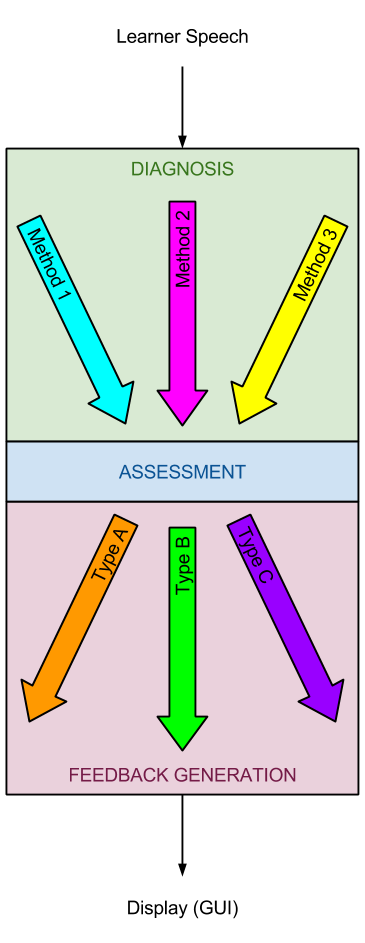
\includegraphics[width=.35\textwidth]{../img/hourglass}
%			\vspace{1em}
%			\caption{Conceptual diagram of the prototype CAPT tool.}
%			\label{fig:hourglass}
%			%\vspace{1em}
%		\end{floatingfigure}

The main objective of this work is to investigate the automatic treatment of lexical stress errors in the context of a CAPT system for French learners of German. This includes, on the one hand, an examination of the ways in which lexical stress errors of the type made by French L1 speakers when speaking German as L2 can be reliably detected and measured %TODO reword
automatically, and on the other, an exploration of the types of multimodal feedback on such errors that can be automatically delivered based on the aforementioned error detection. 
%
	\begin{figure}[thb] 
		\centering
		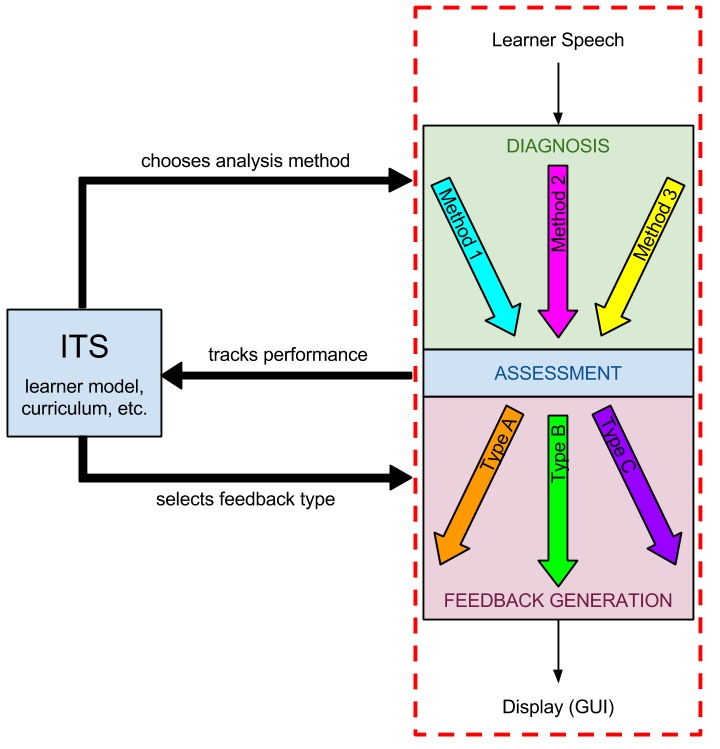
\includegraphics[height=.45\textheight]{../img/hourglass-ITS} 
		\caption[Conceptual diagram of the prototype lexical stress CAPT tool]{Conceptual diagram of the prototype lexical stress CAPT tool (demarcated by dotted line) and its possible function in the context of a more comprehensive Intelligent Tutoring System.}
		\label{fig:hourglass-ITS}
	\end{figure}
%
The outcome of these investigations is a prototype CAPT tool, illustrated in \cref{fig:hourglass-ITS},
which can diagnose lexical stress errors in different ways and present learners with different types of feedback on these errors.

This prototype tool has been developed with both instructional and research applications in mind.
Unlike with some existing tools for diagnosis pf and feedback on pronunciation errors, learners can interact with the tool and interpret its feedback independently, i.e. without the assistance of a human instructor at their side.
At the same time, researchers can use this modular system to study the impact of various assessment and feedback types on learner outcomes, user engagement, and other factors impacting the success of a CAPT system. 
%
Once more is known about which diagnosis/feedback types should be delivered to which learners in which situations, this tool could become a useful component to a fully-fledged CAPT system, in which learner models and other intelligent components automatically decide which modules of the tool to activate. 



\section{Thesis overview}
\label{sec:intro:overview}

\TODO{Add chapter names?}

\myemph{\Cref{chap:background}} introduces Computer-Assisted Pronunciation Training (CAPT) in the contexts of pronunciation teaching in foreign-language education and computer-based and intelligent tutoring systems, describing some relevant past work on CAPT systems. This chapter also briefly 
%outlines the differences in the lexical stress systems of French and German as well as 
introduces the phenomenon of lexical stress as it pertains to L1 French learners of German as L2, and outlines
the motivation for focusing on lexical stress errors in this work.

%TODO flesh out

\myemph{\Cref{chap:lexstress}} 
%explores lexical stress in the speech systems of French and German in more detail, describing relevant findings from past work on lexical stress and its acoustic correlates in these languages. 
%This chapter also 
describes original work on the annotation and analysis of lexical stress errors in the IFCASL sub-corpus of nonnative German speech produced by native French speakers.

\myemph{\Cref{chap:diagnosis}} details how the prototype CAPT tool diagnoses lexical stress errors in learner speech. It describes the methods used to automatically segment the learner's utterance, analyze the prosody of this utterance in terms of the relative pitch, duration, and intensity of the relevant syllables, and compare this analysis to one or more models of native pronunciation to produce a diagnosis.

\myemph{\Cref{chap:feedback}} describes the multimodal feedback options that the system can deliver, and how these feedback types are generated based on the analysis of the learner's speech described in the previous chapter. 

\myemph{\Cref{chap:system}} briefly introduces the tools that have been developed, and the technology used to build them. \TODO{skip this chapter?}

\myemph{\Cref{chap:conclusion}} summarizes the contributions of this work and outlines some 
possible directions for future work.
%interesting future directions to build on these contributions. %TODO rephrase that



%\section{Proposal overview}
%The remainder of this proposal is structured as follows.
%
%TODO update - this is the old overview from the proposal
%\Cref{chap:background} places this thesis in the context of existing research on CAPT, and motivates its specific focus on lexical stress errors.
%\Cref{chap:diagnosis} outlines the techniques to be explored for diagnosing lexical stress errors in learners' speech via automatic processing of acoustic correlates of these errors in a spoken utterance.
%\Cref{chap:feedback} describes the multimodal feedback types the system will aim to deliver, 
%%and how these could be generated automatically from 
%based on
%the analysis described in the previous section.
%\Cref{sec:conclusion} summarizes the proposal and the aims of the thesis.

 		% INCLUDE: introduction

%\part{Background}
% BACKGROUND & RELATED WORK
%
% !TEX root = ../thesis-main.tex
%
\chapter{Background and related work}
\label{chap:background}

%\cleanchapterquote{You can’t do better design with a computer, but you can speed up your work enormously.}{Wim Crouwel}{(Graphic designer and typographer)}

As stated in the previous chapter, the work reported this thesis aims to make progress towards the development of Computer Assisted Pronunciation Training (CAPT) system for learners of German as a foreign language (L2), with a particular focus on learners whose native language (L1) is French. This work therefore draws from and builds upon research in diverse but related fields, including L2 education, language technology, and phonetics/phonology.

This chapter sets the stage for the original work described in the remainder of the thesis by summarizing some relevant previous research on pronunciation in foreign language teaching and CAPT, describing the phenomenon of lexical stress as it relates to the comparative word prosody of German and French, and motivating this work's focus on lexical stress errors as a type of error well-suited to correction via CAPT.


	\section{Pronunciation in foreign language education}
	\label{sec:bkgd:l2ed}
%	
%	The difficulties posed by including pronunciation in the foreign language classroom curriculum will be discussed in this section, leading to the conclusion that CAPT can help make pronunciation training more accessible by overcoming some of these difficulties (e.g. teacher-to-student ratio). Relevant findings from a variety of works on pronunciation teaching in the classroom will be presented .

%\citep{Derwing2005,Dlaska2013,Hirschfeld2007,Mehlhorn2005}

In the foreign language classroom, and the German language classroom in particular, less focus has traditionally been placed on pronunciation than other aspects of language education, such as grammar and vocabulary %; %\citep{Neri2002,Derwing2005}. 
%this is particularly true for German 
\citep{Hirschfeld2007}.
However, even when pronunciation is taught in the classroom, a number of factors may limit the effectiveness of that training. %\citep{Neri2002,Derwing2005}. 
First of all, partly thanks to a historical lack of communication between the fields of speech science and foreign language education, many teachers lack the training in phonetics and phonology to provide helpful feedback to students and correct their articulation \citep{Derwing2005,Hirschfeld2007}. Secondly, high student-to-teacher ratios may prevent teachers from giving adequate attention and feedback to individual students, and limit the amount of time each student can practice speaking \citep{Neri2002}. Furthermore, anxiety about speaking the L2 in front of their peers may make students less willing to practice speaking, and less able to absorb corrective feedback \citep{Neri2002}. 
%\TODO{individual/specific citations for each point above? Hirschfeld?}



%Fortunately, recent years have seen a growing interest in sound pronunciation pedagogy in the FLE community 

Although much work still needs to be done to improve our understanding of how best to teach pronunciation, existing research reveals a few general considerations that must be kept in mind.
	First of all, it is important to note that 
intelligibility, and not lack of a ``foreign accent,'' is generally considered to be the most important goal of pronunciation training \citep{Munro1999,Neri2002,Derwing2005,Field2005,Witt2012}. %\TODO{\citep{Hahn2004}?}
As \textcite{Field2005} and others point out, the exact definition of the term \textit{intelligibility} is a topic of debate in the literature, as is the question of whether and how it differs from the notion of comprehensibility; 
here, let us follow \textcite[p.~289]{Munro1999} in understanding intelligibility broadly as ``the extent to which a speaker’s message is actually understood by a listener.'' 
%here, intelligibility is understood broadly as the degree to which the \TODO{content} of the (L2) speaker's utterance is made clear to the listener.
	

Research on the impact of various types of pronunciation errors on intelligibility tends to indicate that errors on the prosodic (suprasegmental) level may hinder intelligibility more than segmental errors.
% 
In a study of nonnative English speakers from various native language (L1) backgrounds, \textcite{Anderson-Hsieh1992} found that overall pronunciation ratings, which reflect intelligibility, correlated more strongly with measures of prosodic accuracy than with accuracy with respect to segmental sounds or syllable structure.
%
Later research by \textcite{Hahn2004} points to the particular importance of primary sentence stress, e.g. the accentuation of new or contrasting words in a given sentence, to the intelligibility of L2 English speakers, especially with respect to the way in which these speakers (fail to) use intonation to convey stress.
%
%\TODO{\citep{Derwing2005}}
%
%\TODO{lexical stress errors have been found to impact intelligibility when the L2 is German is the L2 \citep{Hirschfeld1994,Hirschfeld2007}}
Though there exists relatively little research on the impact of various pronunciation errors on intelligibility in German specifically, some studies suggest that prosodic errors, and lexical stress errors especially, may hinder intelligibility of L2 speech more than other types of errors \citep{Hirschfeld1994,Hirschfeld2007}.



To reduce these and other types of errors in learner speech,
%training (e.g. in the form of listening exercises) which helps 
listening exercises designed to help 
learners perceive phonological phenomena in the target language
%between correct and erroneous pronunciations
%has 
have been found to be valuable, with some work suggesting that perception training can have a positive impact on the intelligibility of L2 speech, even in the absence of exercises or feedback concerned with production \citep{Derwing2005,Hirschfeld2007}.
%
However, 
%some researchers stress 
other research suggests that production-oriented training with corrective feedback on pronunciation errors produces bigger performance gains. %\citep{Dlaska2013}. 
%\TODO{expand}
%
%\TODO{transition} he importance of individualized corrective feedback is also generally acknowledged.
%\citep{Neri2002,Mehlhorn2005,Dlaska2013}, 
%
%\TODO{\citep{Neri2002}}
As \textcite{Neri2002} point out, corrective feedback from human instructors has been shown to help adult L2 learners notice errors in their pronunciation more than implicit feedback in the form of exposure to speech from L1 speakers of the target language, enabling them to start working towards correcting these errors and thus improving their pronunciation.
This supports the claims of \textcite{Mehlhorn2005} regarding the importance of individualized pronunciation coaching as a way to help L2 German learners become more cognizant of their pronunciation deviations as they take autonomous control of their own pronunciation learning.
%
%\TODO{corrective fb more important than perception training (or stg?) \citep{Dlaska2013}} \TODO{Explicit FB is necessary; learners have trouble identifying their errors when simply asked to listen to what they said \citep{Dlaska2013}}
In a study of L2 German speakers from a variety of L1 backgrounds, \textcite{Dlaska2013} compared the effects of implicit and explicit feedback on the improvement in comprehensibility of the L2 learners' speech, and found that individualized, explicit, corrective feedback from a human language instructor led to more substantial improvements in comprehensibility than the implicit feedback of listening to the learner's own recorded utterance or that of a model native speaker; their findings seem to point to the difficulties learners may have in identifying their own errors, and confirm the importance of offering explicit feedback in L2 pronunciation instruction. 
%

It is thus generally evident that individualized corrective feedback is quite important for L2 pronunciation learning, including L2 German learning specifically; however, there remains much to be learned about exactly when and how feedback can be most effective. This is the motivation behind the 
%feedback generation module of the proposed tool 
diversity of feedback types implemented in the \TODO{de-stress} 
%Computer-Assisted Pronunciation Training (CAPT) 
system (see \cref{chap:feedback}); as described in the previous chapter, this system is intended to facilitate finer-grained research on the effects of such feedback on the acquisition of L2 German word prosody by L1 French speakers.




%TODO \vfill?


\section{Computer-Assisted Pronunciation Training}
\label{sec:bkgd:capt}


In recent decades, the educational value of speech technologies has been well demonstrated \citep{Eskenazi2009}, with 
Computer-Assisted Pronunciation Training%
\footnote{Also known as Computer-Assisted Pronunciation Teaching or Tutoring} (CAPT) 
emerging as one important educational application for foreign-language education (FLE) \citep{Neri2002,Delmonte2011,Witt2012}. 
%Computer-Assisted Pronunciation Training\footnote{Also known as Computer-Assisted Pronunciation Teaching or Tutoring} (CAPT) stands to help make pronunciation training more accessible by overcoming some of these difficulties. 
With CAPT, student-to-teacher ratio is not an issue, as the learner always has the full attention of the digital tutor, and provided an effective curriculum design, a CAPT system can offer learners practically limitless practice opportunities. Interacting with a computer program may also be perceived by the learner as a lower-stakes, more comfortable environment than the classroom, where they may feel too intimidated to practice speaking in the L2 \citep{Neri2002}. But perhaps most compelling is the potential for CAPT 
to deliver the type of individualized instruction
%guided by sound science and pedagogy 
which many learners may not otherwise have access to in the L2 classroom, for reasons such as those mentioned in \cref{sec:bkgd:l2ed}.
%Much of the recent interest in CAPT stems from its potential to deliver the type of individualized pronunciation instruction, guided by sound science and pedagogy, which many learners may not have access to in the classroom, as just discussed.
%
%Indeed, in recent decades, the educational value of speech technologies has been well demonstrated \citep{Eskenazi2009}, with CAPT emerging as one important educational application for foreign-language education (FLE) \citep{Neri2002,Delmonte2011,Witt2012}. 
%	%CAPT is attractive from the pedagogical perspective, as its potential to deliver individualized, extended practice poises it to overcome some of the hurdles of teacher-led pronunciation training described in \cref{sec:bkgd:l2ed} below \citep{Neri2002,Derwing2005}. 
However, as \textcite{Derwing2005} point out, for CAPT to be effective, it must be informed by research on not only speech technology, but both speech production and perception on the one hand, and language acquisition and pedagogy on the other.
With this in mind, an overarching aim of this thesis is to take initial steps toward the development of German CAPT technology which takes into account information from these diverse fields. 
%	This section places CAPT in the context of foreign-language pronunciation instruction (\cref{sec:bkgd:l2ed}), and describes a few recent CAPT systems which incorporate training in prosody (\cref{sec:capt:systems}). \TODO{why prosody?}
%
%	
%
%
%	\subsection{Computer-based and intelligent tutoring systems?} 
%	\label{sec:capt:its}
%	%TODO is this section necessary?
%	
%	This section would serve as a domain-independent overview of CBT and ITS, and the advantages such systems can bring when deployed in schools or used individually.
%	
   % \subsection{Prosody in existing CAPT systems}
	\label{sec:capt:systems}
		
	The viability of CAPT has been demonstrated by a variety of systems and tools that have been developed in both academic and commercial contexts. Some focus on overall assessment of pronunciation or fluency, and others on the detection and correction of individual pronunciation errors \citep{Eskenazi2009}; the tool developed in this work falls into the latter category. In error-focused systems, a distinction has typically been drawn between phonemic errors, e.g. the substitution, insertion, or deletion of a segmental speech sound, and prosodic errors, such as those related to stress/accent, intonation, or rhythm \citep{Witt2012}. As discussed in the previous section, word-prosodic errors may have a larger impact on intelligibility than segmental errors, and are therefore the focus of this work (see \cref{sec:bkgd:targeting} below). 
	With this in mind, a few prosody-aware CAPT systems relevant to this thesis are discussed below (\cref{sec:capt:snoori,sec:capt:fluency,sec:capt:listen,sec:capt:german}); comprehensive overviews and comparisons of these and many other systems are given by \textcite{Neri2002,Eskenazi2009,Delmonte2011,Witt2012}.  
	
	
		Additionally,
		both the diagnosis and feedback modules of the \TODO{de-stress} CAPT tool developed in this thesis project build to a great extent on previous work by researchers in the speech group at LORIA\footnote{\url{http://www.loria.fr/}} in Nancy, France, many of whom are also involved in the IFCASL project (see \cref{sec:intro:ifcasl}). 
		One relevant body of work at LORIA has investigated the task of automatically recognizing and segmenting learners' speech, and determining how this possibly incorrect automatic segmentation can be effectively utilized in the context of pronunciation tutoring; this work is summarized in \cref{sec:capt:auto}. Furthermore, the group has developed the Snorri suite of speech analysis software, described in \cref{sec:capt:snoori}, the most current version of which, JSnoori, has provided the foundation for many elements of \TODO{de-stress}.
		
	
	%\subsubsection{Automatic processing of learner speech}
	\subsection{Automatic processing of learner speech}
	\label{sec:capt:auto}
	
	
	An important prerequisite of any useful CAPT system is the capability to process learner speech automatically. This may be attempted via the application of general techniques for automatic speech recognition or automatic alignment of read speech, but given the drastic ways in which L2 speech typically differs from that of L1 speakers, additional measures must usually be taken to ensure that learners' utterances can be processed reliably and robustly.
	%
	Over the past decade or more, researchers at LORIA have been advancing the state of the art for nonnative speech processing, particularly in the context of CAPT applications 
	(e.g. \cite{Bouselmi2005,Bouselmi2012,%
	Mesbahi2011,Orosanu2012,Jouvet2011,Bonneau2012}); this section provides an overview of that work.
	
	
	One approach to improving recognition accuracy on L2 speech explored by these researchers involves modifying or adapting the L1 acoustic models used for recognition to better cope with L2 speech data. \textcite{Bouselmi2005} found that merging acoustic models trained on native speech in the target language (English, in their evaluation) with models trained on speech in the learner's L1 (e.g. French) resulted in better recognition accuracy on L2 speech, and in later work (\citeyear{Bouselmi2012}) achieved additional improvements in accuracy 
	%by not only adapting the L1 acoustic models for each phone but also 
	by modeling nonnative pronunciation errors (e.g. the insertion, deletion, or substitution of a phoneme) via the automatic extraction of non-standard pronunciations from a corpus of L2 speech. Whereas \textcite{Bouselmi2012} explored the use of L2 pronunciation variants at the level of acoustic modeling, other research at LORIA has shown that augmenting the pronunciation lexicon with nonnative pronunciation variants can also be an effective way of improving the accuracy of L2 speech recognition \citep{Jouvet2011,Mesbahi2011,Bonneau2012}. \textcite{Mesbahi2011} evaluated the segmentation boundaries (i.e. starting and ending points of each phone in the utterance) automatically produced using a lexicon with nonnative pronunciation variants, and found that these were for the most part quite close to (within 15 milliseconds of) the boundaries placed manually by trained scientists, and concluded from this that such automatically-produced segmentations are reliable enough for use in CAPT. 
	
	\TODO{Remove this whole paragraph? Move to future work?}
	Though these adaptation techniques thus reduce the number of errors in the automatic segmentation of L2 speech, some errors still remain as a result of more profound deviations between the expected utterance and that actually produced by the learner. For example, learners may insert or delete not only individual phones, but entire syllables; they may hesitate or repeat words or parts thereof; and they may pronounce words or phrases entirely different from the expected text. \textcite{Bonneau2012,Orosanu2012} explored methods for detecting errors like these by comparing two segmentations: one produced by forced alignment (see \cref{sec:diag:segmentation}), in which the recognition task is constrained by the text of the expected utterance, and the other produced by unconstrained phone-level recognition (phone decoding). 
	By detecting deviations between these two segmentations in a pre-processing step, a CAPT system would be able to catch aberrant utterances before automatic segmentation is attempted, so that the learner can be asked to record their utterance again.
	
	
		
	%Both the diagnosis and feedback modules of \TODO{the CAPT tool} developed in this work build to a great extent on previous work by researchers in the speech group at LORIA\footnote{\url{http://www.loria.fr/}} in Nancy, France, many of whom are also involved in the IFCASL project (see \cref{sec:intro:ifcasl}). 
	%
	% \TODO{\textit{This part about segmentation doesn't really fit in with the prosody-in-CAPT discussion - find a better place for it.}}
%	 Their work has, on the one hand, investigated the task of automatically recognizing and segmenting learners' speech, and determining how this possibly incorrect automatic segmentation can be effectively utilized in the context of pronunciation tutoring, particularly at the prosodic level \citep{Mesbahi2011,Orosanu2012}; \TODO{details}
	%TODO {see \cref{chap:diagnosis} for a discussion of how this thesis will build upon that work. \textit{Details \& de-proposal-ize}}
	
	%\TODO{\citep{Bouselmi2005,Bouselmi2012}}
	
	%\TODO{\citep{Bonneau2012}}
	
	%\sub
	\subsection{The Snorri suite and JSnoori}
	\label{sec:capt:snoori}
	
	%Additionally, the group has developed
	Another contribution of the LORIA group vital to this thesis project is 
	the Snorri suite of software, 
	which includes the now-outdated original Snorri developed in 1987 \citep{Fohr1989} and a Unix adaptation developed shortly thereafter,
	a later Windows port of Snorri appropriately called WinSnorri \citep{Laprie1999},
	%and its partial Java port, JSnoori {Parole2013}, 
	and most recently a partial Java port of WinSnorri, JSnoori\footnote{\url{http://jsnoori.loria.fr}} \citep{Parole2013}. 
	JSnoori is the incarnation of the Snorri suite which is still under active development and is 
	%the version of the Snorri suite 
	most relevant to this work.

	
	The screenshot in \cref{fig:jsnoori:screenshot} depicts JSnoori's interface for speech analysis. In this example, a recording of a native speaker utterance of the French sentence ``Mon ami a perdu ses bagages à la gare'' (\textit{My friend lost his luggage at the train station}) is under analysis, with only the portion of the signal corresponding to the word ``perdu'' (\textit{lost}) visible.  At the bottom of the screen, in grey, the phone-, word- and sentence-level segmentations of the utterance are displayed. The oscillogram (waveform) of the selected portion of the speech signal is visible as a red contour above the segmentations.  In the upper portion of the screen, a spectrogram of the selected signal segment is presented, with overlaid, colored contours corresponding to the fundamental frequency (blue dots) and intensity (green line) of the signal. Controls at the top of the window allow the user to listen to the selected recording and utilize the various speech analysis capabilities of the software.
	
	Like its predecessors Snorri and WinSnorri, JSnoori offers users a wide array of signal processing and visualization features, as described by \textcite{Fohr1989,Laprie1999}. 
	In addition to basic signal recording, editing, and playback, the software can also be used to segment and annotate speech recordings manually or automatically (see \cref{sec:capt:auto}). 
	Users can choose among various types of spectral visualizations, including wide- or narrow-band spectrograms and cepstrally smoothed spectrograms. 
	Sophisticated pitch detection algorithms (see \cref{sec:prosody:f0}) enable the analysis and visualization of fundamental frequency (F0) 
	%and formant structure 
	in the signal. 
	JSnoori also allows users to prosodically modify a given speech signal by altering the duration or pitch contour of that signal or a portion thereof; see \cref{sec:implicit:auditory:resynth} for a more detailed explanation of the techniques used to accomplish this modification.
	
	
	\begin{figure}
		\centering
		\caption[Screenshot of the speech-analysis interface of JSnoori]{Screenshot of the speech-analysis interface of JSnoori.
		%depicting a segment of a French utterance corresponding to the word ``perdu'' (\textit{lost}). 
		%At the bottom of the screen, in grey, the phone-, word- and sentence-level segmentations of the utterance are displayed. The oscillogram (waveform) of the selected portion of the speech signal is visible as a red contour above the segmentations.  In the upper portion of the screen, a spectrogram of the selected signal segment is presented, with overlaid, colored contours corresponding to the signal's fundamental frequency (blue dots) and intensity (green line). Controls at the top of the window allow the user to listen to the selected recording and utilize the various speech analysis functions of the software.
		}
		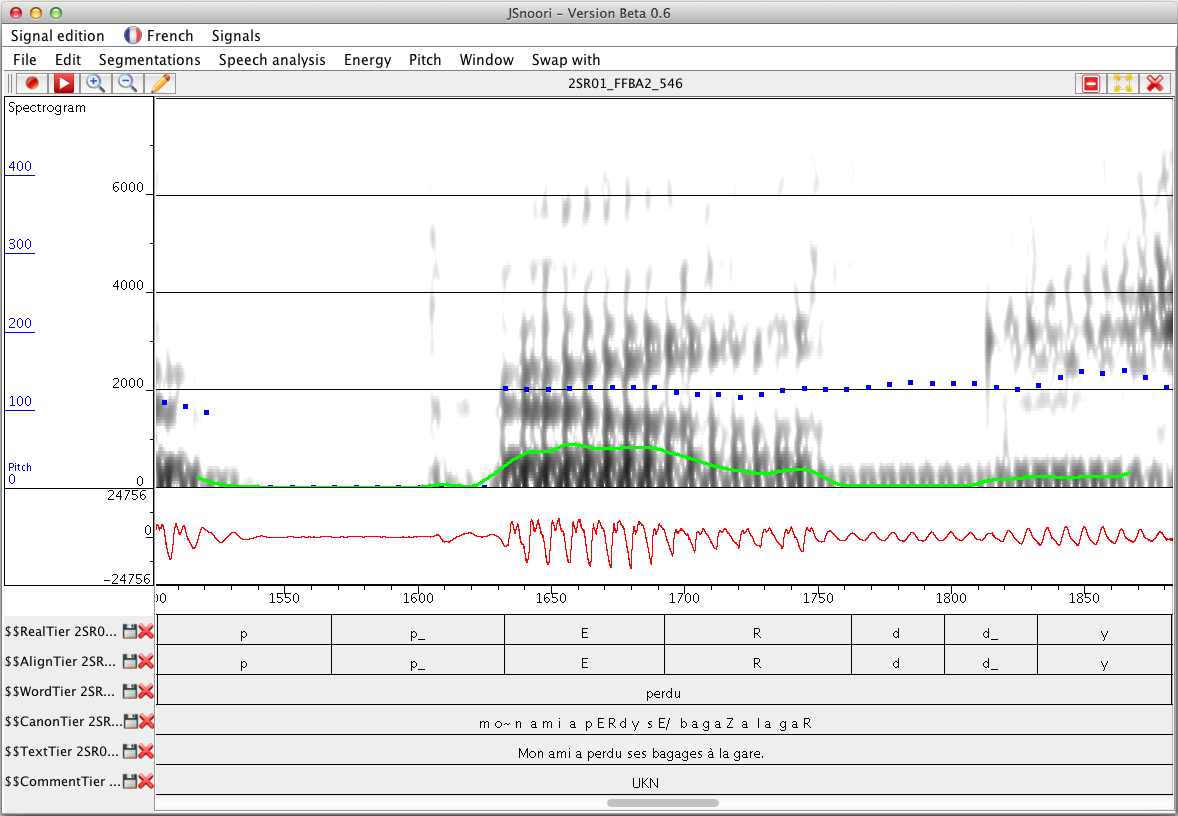
\includegraphics[width=\textwidth]{img/screenshots/JsnooriScreenshot}
		\label{fig:jsnoori:screenshot}
	\end{figure}
	
	Though the Snorri programs were originally developed primarily as research tools for speech scientists %\TODO{\textit{necessary to cite again so soon?} 
	\citep{Fohr1989,Laprie1999}, 
	the utility of such software
	%, and especially of resynthesized feedback, 
	for pronunciation teaching has been explored by the LORIA team \citep{Bonneau2004,Henry2007,Bonneau2011},
	% \citeauthor{Bonneau2004} (\citeyear{Bonneau2004,Bonneau2011}) \TODO{add \citep{Henry2007}},
	% \textcite{Bonneau2011}, 
	who have used 
	%\TODO{\textit{correct?} WinSnoori} 
	this software to assess lexical stress in L1 French speakers' pronunciation of English words, and deliver feedback on learners' errors. 
	%
	%\TODO{transition}
In its role as a CAPT tool, JSnoori (like its predecessor, WinSnoori)
takes as input a learner utterance, a native reference utterance, and segmentations of each, performs an acoustic comparison of the two utterances, and delivers feedback 
%on the learner's speech 
in the form of e.g. annotated displays of the speech signal and spectrogram of each utterance. Moreover, auditory feedback can be delivered 
%thanks to the capability of 
by
resynthesizing the learner's utterance to match the pitch contour and timing of the reference, without modifying the voice quality of the utterance, such that the learner can hear the ``correct'' pronunciation in their own voice (see \cref{sec:implicit:auditory:resynth} for details). 

	A pilot experiment conducted by \textcite{Bonneau2011} used WinSnoori to investigate the effect of these types of visual and auditory feedback on the prosodic realization of English lexical stress by L1 French learners, and seemed to indicate that this feedback has a beneficial effect for learners with a low proficiency level in the L2 (i.e. beginners), whereas more advanced learners seem to improve their pronunciation just as well when simply allowed to listen to a reference utterance recorded by a native speaker as a form of implicit feedback. However, as all of the feedback types available were presented simultaneously to learners in the experimental condition, further research is needed to determine whether there are differences in efficacy among the individual feedback types; enabling such research is the motivation behind the modular feedback component of \TODO{de-stress} (see \cref{chap:feedback}).

	

As described in \cref{chap:diagnosis,chap:feedback}, 
the JSnoori software is vital to this thesis project;
\TODO{de-stress}
%the prototype CAPT tool developed in this work 
utilizes the signal processing capabilities of JSnoori 
%and
%builds on the error diagnosis functionality of JSnoori 
for speech analysis and error diagnosis (see \cref{chap:diagnosis}), 
and leverages its feedback generation capabilities to deliver  a more diverse, and potentially more effective, range of feedback types (see \cref{chap:feedback}). 
	
	% \citep{Bonneau2011,Fohr1996,Fohr2012,Mesbahi2011,Orosanu2012}. The JSnoori/WinSnoori software \citep{Parole2013}
%which this group has developed will be instrumental in the construction of the CAPT tool. 

	%\sub
	\subsection{The Fluency pronunciation trainer}
	\label{sec:capt:fluency}
	
	This work also draws from research on two systems developed at Carnegie Mellon University.
%, namely the Fluency pronunciation trainer
%\citep{%
%	%Eskenazi1998,%
%	Eskenazi2000,%
%	%Probst2002%
%	} 
%and the Project LISTEN Reading Tutor \citep{%
%	%Mostow1999,	
%	%Duong2011,
%	%Sitaram2011,
%	Mostow2012,
%	%Weber2010
%	}. 
%
	The first of these, the Fluency pronunciation trainer \citep{Eskenazi1998,Eskenazi2000}, is a CAPT system placing particular emphasis on
%prosody and 
user-adaptivity, corrective articulatory feedback, and the integration of perceptual training (e.g. listening exercises). As with the work at LORIA described above, the Fluency system evaluates learners' speech via comparison with that of a native reference speaker; \textcite{Probst2002} found that selecting a ``golden speaker'' whose voice closely matched the learner's improved learning gains, a finding which informed the implementation of various reference speaker selection methods in the diagnosis module of \TODO{de-stress} (see \cref{sec:compare:selection}).
Fluency also implements an error-catching step to reject utterances which do not match the expected text \citep{Eskenazi2000}, in the same vein as that of \textcite{Mesbahi2011,Orosanu2012}. \textcite{Eskenazi2007} report that Fluency's commercial spin-off, NativeAccent\textsuperscript{TM}, has been shown to help real-world users significantly improve their pronunciation skills.
	%In an early version of Fluency, an utterance is elicited from the learner using a targeted question, constraining the learner's response such that a speech recognizer can perform forced alignment on the utterance, while at the same time giving the learner the impression that they have decided what to say (as opposed to simply reading a given sentence out loud).
	
	%\sub
	\subsection{The Project LISTEN Reading Tutor}
	\label{sec:capt:listen}
	
	A second CMU system, the Project LISTEN Reading Tutor \citep{Mostow2012} 
may not strictly be a CAPT tool, as it 
is designed to help children develop reading fluency in their native language. 
However, as 
%To that end, 
it analyzes the prosody of children's read speech to measure reading fluency, and offers feedback on this prosody, 
it is nevertheless very relevant to CAPT and thus this thesis. 
	Indeed, the potential for such a tool, and its underlying technologies, to enhance foreign-language education has already been demonstrated by 
	\textcite{Weber2010}, who deployed the Reading Tutor in English as a second language classes in India with encouraging initial results. 
	As this section explains, ideas and techniques from the Reading Tutor have influenced both the diagnosis and feedback modules of the proposed CAPT tool. 
	
	
	In the Reading Tutor, the child's read speech is automatically segmented and compared either to a reference utterance by an adult reader, analogous to the native speaker reference in many CAPT systems, or to a generalized model of adult prosody. \textcite{Duong2011} report better performance using the generalized model, a result which motivated \TODO{de-stress}'s implementation of a classification-based alternative to the more typical comparison-based method of error diagnosis (see \cref{sec:diag:classification}).
	
	 The Reading Tutor's analysis of the pitch and intensity contours of the utterance(s), as well as the duration of words/syllables and the pauses between them, results in an assessment of the child's overall fluency as well as identification of words which have been pronounced (in)correctly, and feedback is delivered visually in real time by revealing the text of each word as it is spoken, with properties such as the position, color, and font size of each word reflecting various aspects of the reader's prosody \citep{Sitaram2011}. Inspired by this work, a similar method of feedback via text stylization has been implemented in \TODO{de-stress} (see \cref{sec:implicit:visual:text}). 
	
	\subsection{German and language-independent CAPT}
	\label{sec:capt:german}
	%\TODO{flesh out this paragraph - rephrase subsection heading?}
	The vast majority of CAPT systems which analyze learners' speech at the prosodic level have been developed with English as the target L2. In contrast, relatively little work has been done on prosody-oriented CAPT in German.
	However, work by \textcite{Jilka1998} on L2 German speech produced by L1 English speakers also suggests that manipulating the intonation contours of learner utterances may be an effective way to provide corrective feedback on intonational errors contributing to a perceived foreign accent in German, and  
	%
\citeauthor{Bissiri2006} 
(\citeyear{%
%\citep{%
Bissiri2006,Bissiri2009%
})
 found that L1 Italian speakers' realizations of lexical stress in German improved when they were allowed to listen to 
prosodically-modified recordings of their own speech and that of native speakers. 
	Based on these findings, feedback via resynthesis may be a very useful element of a German CAPT system, and such feedback is therefore one of the types implemented in \TODO{de-stress} (see \cref{sec:implicit:auditory:resynth}).
%their own utterance resynthesized to reflect the prosody of a reference utterance by a native speaker, as well as when they could listen to an utterance by a native speaker that had been prosodically modified to place 
%prosodically-modified auditory feedback useful for improving L1 Italian speakers' realizations of lexical stress in German \TODO{What did they find out?}.
%
	%\citeauthor{Jilka1998}'s (\citeyear{Jilka1998}) use of F0 contour manipulation in studying L1 English speakers' production of German represents another exploration of speech technology applications for German instruction. \TODO{details}
	%Work by \textcite{Jilka1998} on L2 German speech produced by L1 English speakers also suggests that manipulating the intonation contours of learner utterances may be an effective way to provide corrective feedback on intonational errors contributing to a perceived foreign accent in German, and  
	%
%	Ville, for L2 Swedish instruction \citep{Wik2009}, incorporates both perception and production exercises for lexical stress and other prosodic errors, and features an animated virtual character as the tutor.
%
	%\TODO{Delmonte's SLIM?}, 


	Language-independent tools have also been developed for teaching prosody, such as WinPitch LTL \citep{Martin2004}, which enables speech signal visualization of prosodic features such as pitch contours as well as manipulation of prosody and comparison to reference utterances, with the intent that a human instructor will guide the learner in using the software and interpreting the visualizations. Unfortunately, as \textcite{Neri2002} point out, the necessity of having an instructor help the learner interpret the visual and auditory feedback provided by this software negates one primary advantage of CAPT:
	%, mentioned in \cref{sec:bkgd:capt}: 
	the ability to offer learners feedback in situations where individualized attention from a human instructor is limited, which is often the case in foreign language classrooms, as explained \cref{sec:bkgd:l2ed}.
	%\TODO{anything else?}
	
	%Other systems mentioned by \textcite{Eskenazi2009,Delmonte2011,Witt2012} may also be briefly described, including tools developed at KTH \citep{Hincks2002,Hincks2009} to teach English prosody.
	
	%\TODO{need an outro for this (sub)section?}
	
	
% Alternative organization:
 \section{Lexical stress}
 \label{sec:bkgd:stress}
		%TODO check this section for inaccuracies
		When there is a typological difference between some segmental or prosodic feature(s) of a language learner's L1 compared to the target L2, there is a particular need for pronunciation training to bridge this gap. In the case of the French-German language pair, the prosodic realization of lexical stress is one feature which marks a striking difference between the languages.
		
			In the broadest terms, lexical stress is the phenomenon of how syllables are accentuated within a word  \citep{Cutler2005}. To say that a given syllable in a word is stressed is, generally speaking, to say that that syllable is somehow accorded a more prominent role in the word than other syllables, i.e. that this syllable is perceived as somehow ``standing out'' \citep{Dogil1999}.
			%\TODO{Elaborate} 
			The perceived prominence of a syllable in a word is a function not merely of the segmental characteristics of the uttered syllable, i.e. the speech sounds it contains, but rather of its (relative) suprasegmental properties, namely: %TODO need citation here?
			\begin{itemize}
			\item duration, which equates on the perceptual level to length; %timing;
			\item fundamental frequency (F0), which corresponds to perceived pitch; and
			\item intensity (energy or amplitude), which perceptually equates to loudness.
			\end{itemize}

%TODO more text here? or move text from German vs French section here?
	\subsection{German}
	\label{sec:stress:german}
	
		
		%\subsection{German vs. French}
		%\label{sec:stress:GvF}
		
					As \textcite{Cutler2005} points out, different languages make use of this suprasegmental information in different ways.
			In what are termed free- or variable-stress languages, such as German, Spanish, and English, it is not always possible to predict which syllable in a word will carry the stress, and therefore knowing a word requires, in part, knowing its stress pattern. This allows lexical stress to serve a contrastive function in these languages, such that two words may share exactly the same sequence of phones and nevertheless be distinguished exclusively by their stress pattern, as is the case with \textit{UMfahren} (to drive around) and \textit{umFAHRen} (to run over with a car) in German. %TODO better example of minimal pair
Because stress carries meaning thus, native speakers of such languages are sensitive to stress patterns, and readily able to perceive differences in stress. %TODO wording?
Furthermore, in German, misplaced stress has been shown to disrupt understanding of a word or utterance even in cases where there is no stress-based minimal pair \citep{Hirschfeld1994}, supporting the theory that speakers of free-stress languages rely to a large extent on stress information in the recognition of spoken words \citep{Cutler2005}.

	\subsection{French}
	\label{sec:stress:french}

			However, in the so-called fixed-stress languages, stress is completely predictable, as it always falls on a certain position in the word;
%in French, for example, stress is fixed on the word-final syllable, while 
in Czech and Hungarian, stress always falls on the initial syllable. Lexical stress may not be as crucial to the knowledge of a word in these languages as in the free-stress languages. Furthermore, although lexical stress is realized in these languages, the distinction between stressed and unstressed syllables may be weaker than in free-stress languages.
%
 While many theorists place French 
 %has often been placed 
 into this category of fixed-stress languages, pointing to the fact that word-final syllables are always most prominent when a word is pronounced in isolation,
 %although 
 others argue that
 it may be more properly considered a language without lexical stress, insofar as there is no systematic way in which speakers distinguish a certain syllable from others in the word, aside from the fact that French exhibits phrasal accent, expressed as a lengthening of the final syllable in each prosodic group or phrase \citep{Dupoux2008,Michaux2013}.  
 %
 Regardless, stress at the word level does not serve any contrastive function in French \citep[p.~89]{Michaux2013}, 
 %and in fact there may be no feature of French prosody which performs a contrastive function \citep[p.~701]{Dupoux2008}. This 
 which
 constitutes a significant difference between this language and a language with variable, contrastive lexical stress such as German or English. 
 
% 		\TODO{``French does not have contrastive stress: the standard final prominence in isolated words disappears when they are located in non-final position in a larger word group, leaving a word-group final accent... Rather than being contrastive, this `primary' accent has a demarcative function. \citep[p.~89]{Michaux2013}}
			
		\subsection{Expected pronunciation errors}
		\label{sec:stress:expected}
		As a result of this difference in the sound systems of the two languages,
		native speakers of French may generally be expected to lack the sensitivity to stress patterns possessed by native speakers of German. Indeed, this has been borne out by research by \textcite{Dupoux2008},
		%\citep{Dupoux2001,Dupoux2008},
  who found that native French speakers seem to be ``deaf'' to 
  lexical stress, 
  %differences in stress patterns, 
  insofar as they have significant and lasting difficulty
  perceiving 
  %and creating a lasting phonological representation of 
  lexical stress in Spanish, another language in which stress serves a contrastive function.
  %\TODO{\textit{JT comments} discriminating} between Spanish words which contrast only at the level of stress. 
  This difficulty should also exist for French speakers when they are presented with German words in which the stress pattern is crucial to the word's meaning, as in the minimal pair above. 
  
  In addition to these difficulties with lexical stress perception, French learners of variable-stress languages such as English, German and Dutch have also been shown to have difficulties in producing stress patterns correctly. Research by \citeauthor{Michaux2012} et al. (\citeyear{Michaux2012,Michaux2013}) revealed that, as might be expected given the tendency for word- and/or phrase-final syllable prominence in French just discussed, French learners of Dutch  showed a tendency to stress the final syllables of Dutch words, even when not called for by the canonical stress pattern. 
  %\TODO{mention no-stress pattern? happens in English sentence stress with speakers of different L1s \citep{Hahn2004}} 
  Indeed, with regard to German specifically, \textcite{Hirschfeld2007} report that lexical stress errors are commonly observed among L2 speakers with French as L1.
  
% While little research exists specifically investigating the errors of French, 
 In short, based on prior work on French learners of variable-stress languages,
 it can reasonably be expected that L1 French learners of German as L2 will face challenges with both the perception and production of lexical stress, and that the (lack of) lexical stress system in their native language will influence their realization of lexical stress patterns in German words.

		
		
 \section{Targeting lexical stress errors in CAPT}
 \label{sec:bkgd:targeting}
 	Learners of a foreign language typically make a wide variety of pronunciation errors, at both the segmental level (e.g. errors in producing certain vowels or consonants of the target language) and the prosodic level (e.g. errors in the speaker's intonation contour or the duration of certain syllables or words). 
 As it is not feasible to address all of these in a prototype CAPT tool, 
one of the first aims of this work is to identify a single type of error which is well suited to being addressed via CAPT for L1 French/L2 German.
	
	The selection of an error type to address is guided here by
	%To guide this selection, \TODO{we may consider} 
a set of three criteria that such an error must meet; similar criteria are proposed by \textcite{Neri2002,Cucchiarini2009}.
%
First, 
the error must have a significant \textit{impact on the perceived intelligibility} of the learner's speech; 
as the ultimate goal of the system is to help learners communicate more effectively in the L2,
 an error which is commonly made but nevertheless does not impede understanding of the learner's L2 speech, and thus does not hinder communication in the L2, is not an ideal target. 
%
Second,
the error must be \textit{produced relatively frequently} by French L1 speakers in their production of L2 German, as it would be a misuse of resources to design a system addressing an error seldom made by learners. %\citep{Neri2002}.
%
Third,
in order for the CAPT system to provide any meaningful diagnosis and feedback, the error must lend itself to reasonably accurate and reliable  \textit{detection through automatic processing}. 



As illustrated in \cref{fig:errors}, the best error to target with the CAPT system will fulfill all three criteria, rather than only one or two. 
	 For example, vowel quality errors (e.g. an L1 French speaker producing a German /\textipa{@}/ as [\textipa{\oe}]) may occur frequently in the L2 speech and may be relatively easy to detect automatically, but may not have a great impact on the intelligibility of the L2 German speech. On the other hand, equally frequent vowel quantity errors (e.g. the L1 French speaker producing a German long /\textipa{a:}/ as [\textipa{a}]) may have a greater impact on intelligibility in some cases, but may be more difficult to reliably identify automatically.

		%\begin{center}
		\begin{figure}[htb]
			\centering
			\includegraphics[width=.7\textwidth]{img/error-venn}
			\caption{Criteria for selecting errors to target in a CAPT system.}
			\label{fig:errors}
		\end{figure}
		%\end{center}

	Lexical stress errors 
	%\TODO{e.g.} 
	fulfill all three of these criteria, and this error type has therefore been chosen as the target of the proposed CAPT tool. The remainder of this section 
	%justifies 
	presents the reasoning behind 
	that choice. 
	%This thesis proposes that lexical stress errors are a strong candidate for treatment via CAPT, as this type of error meets all three criteria. 
%	
%	
%
%	 

%
%TODO remove
	%Analysis of the typical and expected errors described in \cref{sec:CAPT4FG:comparison} in terms of these criteria reveals that lexical stress errors are a strong candidate for treatment via CAPT, and will therefore be the focus of the prototype CAPT system described in this thesis. The remainder of this section justifies the selection of this type of error by describing how it fulfills the aforementioned criteria as well or better than any other error type.
%	
%
		\subsection{Impact on intelligibility}
		\label{sec:targeting:intelligibility}
		

	First, as mentioned in \cref{sec:bkgd:l2ed} above, errors related to prosody have 
	often
	%generally
	 been found to have a larger impact on the perceived intelligibility of L2 speakers than segmental errors \citep{Hahn2004,Derwing2005,Witt2012}, and several studies have found lexical stress errors in particular to have in impact on L2 intelligibility
	 % to be particularly important for comprehension 
	 in free-stress languages like English, Dutch, and 
	 %our target language, 
	 German \citep{Hirschfeld1994,Cutler2005,Field2005}.
%Also Swedish \citep{Wik2009}	
	%Research on the impact of various types of pronunciation errors has generally shown that errors related to prosody, and especially to stress, have a larger impact on the perceived intelligibility of the L2 speaker than errors on the segmental level \citep{Derwing2005,Witt2012}. 
	Indeed, studies on perception of German L2 speech have found that among a variety of pronunciation error types, lexical stress errors have one of the most drastic impacts on intelligibility \citep{Hirschfeld1994}.
%
	 %\citep{Warren2009}
	%	
		%Native English speakers are sensitive to lexical stress, among other things\citep{Magen1998}
		%\TODO{recall more content when primary SENTENCE stress is correct \citep{Hahn2004}}
	%	
		Furthermore, lexical stress not only impacts intelligibility on the prosodic level, but may also affect perception of segmental errors in the L2 learner's speech; for example, segmental errors occurring in stressed syllables are more noticeable than those in unstressed syllables \citep{Cutler2005,Michaux2012}. 
	%	
		Additionally, some research indicates that prosodic errors such as lexical stress errors may have more of an impact on perceived foreign accent than segmental errors \citep{Hahn2004,Witt2012}; though it must again be stressed that intelligibility is a more important goal than lack of a foreign accent, insofar as perceived accent may contribute to difficulties being understood by native speakers, this relationship between prosody and accentedness also deserves mentioning.
	% ``Prosody errrors in particular tend to contribute to any perceived accent more so than individual phoneme mispronunciations.'' \citep[p.~6]{Witt2012}
		%		

		\subsection{Frequency of production}
		\label{sec:targeting:frequency}

Secondly, we saw in \cref{sec:bkgd:stress} that perceiving contrasts in lexical stress is notoriously difficult for native French speakers \citep{Cutler2005,Dupoux2008}, and given the strong link between perception and production,
%mentioned earlier (\cref{sec:bkgd:l2ed}), 
this is a good indication that L1 French speakers will regularly make lexical stress errors in an L2 with free, contrastive stress, such as German. \textcite{Bonneau2011} report that in a pilot study of L1 French speakers pronouncing English words, lexical stress was frequently misplaced by beginners; given the similarities of the lexical stress systems of English and German compared to that of French, this is another sign that we can expect such errors to be produced frequently.
%
Indeed, an analysis of lexical stress errors in the IFCASL corpus of non-native (L1 French) German speech conducted as part of this thesis project supports the expectation of frequent lexical stress errors in this particular L1/L2 pair: 
%\TODO{verify/reword if necessary: 
errors were observed at all skill levels, though beginners made many more errors than advanced learners. See \cref{chap:lexstress} for a detailed discussion of these findings.
	

		\subsection{Feasibility of automatic detection}
		\label{sec:targeting:autodetect}

Finally, although much research still needs to be done on automatic detection and diagnosis of lexical stress errors (one of the main motivations behind this work; see \cref{chap:diagnosis}), recent work on this problem has shown encouraging results. As mentioned above, several existing CAPT tools incorporate treatment of lexical stress errors (e.g. \cite{Wik2009,Bonneau2011}). 

	Furthermore, in recent years some researchers have reported success in applying machine learning methods to the classification of lexical stress patterns in English words. 
		\textcite{Kim2011} experimented with various classifiers to identify  stress patterns in 3- and 4-syllable English words, and reported accuracy in the 80-90\% range for high-quality recordings of L1 English speech; in pilot experiments with low-quality recordings, however, the authors obtained lower accuracy: 70-80\% on L1 speech and 50-60\% on utterances by L2 speakers.
	\textcite{Shahin2012a} trained Neural Networks to classify stress patterns in bisyllabic words uttered by L1 English children, with the intended application of treating childhood dysprosody, and reported classification accuracy over 90\% for some stress patterns. 


		%Detecting syllable- or word-level errors may be more feasible than detecting phone-level errors: ``One additional challenge in pronunciation error detection is that a phoneme represents the smallest possible unit compared to the syllable, word, and sentence level. The shorter the unit, the higher will be the variability in the judgment of the pronunciation quality.'' \citep[p.~2]{Witt2012}

	\vspace{2em}


	As lexical stress errors thus fulfill the aforementioned criteria for targeting with CAPT, such errors are the focus of the proposed CAPT system. The following sections describe how this thesis project explores automatic diagnosis (\cref{chap:diagnosis}) and feedback generation (\cref{chap:feedback}) for this type of error.		
		
% \section or \subsection{Other related work on lexical stress in CAPT}

% Old section:
%\section{Towards CAPT for French learners of German}
%\label{sec:CAPT4FG}
	
% Alternative organization:
%	\subsection{Targeting errors in CAPT}
%	\subsection{Lexical stress in French and German}
%	\subsection{Targeting lexical stress errors}

% Old organization:
%	\subsection{Phonetic and phonological comparison}
%	\label{sec:CAPT4FG:comparison}
%		\subsubsection{Segments}
%		\subsubsection{Prosody}
%
%			\paragraph{Lexical stress}
%			
%		\subsubsection{Other factors}
%		
%	\subsection{Targeting lexical stress errors}
%	\label{sec:CAPT4FG:targeting}
%
%		\subsubsection{Frequency of production}
%		
%		\subsubsection{Impact on intelligibility}
%		
%		\subsubsection{Feasibility of automatic detection}
%		

\section{Summary}
\label{sec:bkgd:summary}


As this chapter has shown, CAPT is an important application of speech technology for language learning, as it can help overcome typical difficulties with regard to the teaching of L2 pronunciation, and especially prosody, in the German language classroom (\cref{sec:bkgd:l2ed}). The previous research on CAPT and related technologies summarized in \cref{sec:bkgd:capt} has demonstrated numerous ways in which prosodic errors in L2 speech can be automatically detected, 
setting the stage for the exploration of diagnostic methods presented in \cref{chap:diagnosis}.
%
Similarly, the diverse feedback methods explored in the work described in this chapter have provided the inspiration and technological foundations underlying the modular feedback functionality of \TODO{de-stress}, which is the subject of \cref{chap:feedback}.

 Furthermore, this chapter has introduced the phenomenon of lexical stress in the context of L2 German acquisition by L1 French speakers (\cref{sec:bkgd:stress}), and has motivated the selection of this phenomenon as the focus of this thesis project (\cref{sec:bkgd:targeting}). This discussion of lexical stress provides the context for the original work presented in the following chapter, which investigates the prosodic realization of lexical stress by French learners of German in more detail.	% INCLUDE: background
%% CAPT
%
% !TEX root = ../thesis-main.tex
%

\chapter{Computer-Assisted Pronunciation Tutoring}

%\cleanchapterquote{You can’t do better design with a computer, but you can speed up your work enormously.}{Wim Crouwel}{(Graphic designer and typographer)}

\blindtext 
\section{Pronunciation in foreign language teaching}
\blindtext
\section{CAPT systems}
	\subsection{Selecting errors to target}
	\blindtext
		\begin{center}
		\begin{figure}[htb]
			\includegraphics[width=.7\textwidth]{../img/error-venn}
			\caption{Criteria for selecting errors to target in a CAPT system.}
			\label{fig:errors}
		\end{figure}
		\end{center}
	\subsection{Survey of existing CAPT systems}
	
\section{The IFCASL project}
	\subsection{Individualized feedback in CAPT?}
	\subsection{The IFCASL corpus}

 		% INCLUDE: CAPT

% LEXICAL STRESS ERRORS
%
% !TEX root = ../thesis-main.tex
%
%TODO change title? \chapter{Lexical stress errors in the IFCASL corpus}
\chapter{Lexical stress errors by French learners of German}
\label{chap:lexstress}

%\cleanchapterquote{You can’t do better design with a computer, but you can speed up your work enormously.}{Wim Crouwel}{(Graphic designer and typographer)}

%\blindtext

%\section{Stress in German vs. French }
%	\subsection{Comparative prosody}
%	\subsection{Stress ``deafness'' in French}
%	\subsection{Expected errors}
%	
	
%\TODO{Change title?}
%\section{Lexical stress errors in the IFCASL corpus} 

	
	As the previous chapter has shown, lexical stress is a challenging phenomenon for native (L1) French speakers to realize correctly in their nonnative (L2) German prosody, such that pronunciation errors with respect to lexical stress are expected to be produced frequently by this group of German learners.
%
	However, empirical studies of this type of error as produced by French learners of German are quite few in number (see \cref{sec:stress:expected,sec:targeting:frequency}), so one objective of this thesis project was to research to what extent the expected types of lexical stress errors by French speakers of German are actually produced.
	 As the IFCASL corpus (see \cref{sec:intro:ifcasl}) provides valuable data on L2 German speech produced by L1 French speakers, it is a perfect starting point for such investigations; however, given that the existing corpus annotation does not include information on lexical stress errors,
	  a subset of this corpus had to be manually annotated for such errors; the annotation and subsequent analysis of lexical errors in this data, presented in this chapter, constitute a major contribution of this thesis project.
%
	
	
	The first sections of this chapter describe the selection of material to be annotated (\cref{sec:lexstress:data}), the annotators who labeled lexical stress errors in that data (\cref{sec:lexstress:annotators}), and the method by which annotation was performed (\cref{sec:lexstress:method}). 
	
	%Once error judgments had been collected from each annotator, 
	Given the error judgments thus collected, 
	different annotators' judgments of the same utterances were compared to determine the reliability of the annotation, i.e. the agreement between annotators in terms of the labels they assigned to each utterance.
	%, which gives some indication of the general difficulty of the task of diagnosing lexical stress errors in nonnative German speech. 
	\Cref{sec:lexstress:agreement} describes this analysis of inter-annotator agreement, which aims to shed light on the following questions:
	\begin{itemize}[topsep=-1em]
	\item{How reliably can lexical stress errors be identified by
	%Can lexical stress errors be reliably identified by 
	%native German speakers 
	annotators, i.e. to what extent do the judgments of different annotators agree?  (\cref{sec:agreement:overall})}
	\item{Are there differences in how native and nonnative German speakers identify errors?  (\cref{sec:agreement:native})}
	\item{Are there differences in how 
	%expert and novice annotators (those without 
	annotators with different levels of expertise
	(annotation experience or training in phonetics/phonology) identify lexical stress errors?  (\cref{sec:agreement:expert})} 
	\end{itemize}
	%
	As \cref{sec:lexstress:agreement} will show, annotators did not always agree as to whether a given utterance exhibited a lexical stress error or not. Nevertheless, a single ``gold-standard'' label for each utterance had to be selected; \cref{sec:agreement:gold} describes how this was accomplished in cases of disagreement.
	
	Finally, given the gold-standard labels for each utterance, the distribution of lexical stress errors in the annotated data was analyzed; the following questions guided this analysis, which is detailed in \cref{sec:lexstress:results}.
	\begin{itemize}[topsep=-1em]
	\item{Are lexical stress errors observed frequently in the IFCASL data? (\cref{sec:results:overall})}
		\item{Are lexical stress errors observed more frequently with certain word types than with others?  (\cref{sec:results:wordtype})}
	\item{Is there a difference in the frequency of these errors among different groups of speakers, i.e. in terms of skill level, age, or gender? (\cref{sec:results:level,sec:results:agegender})}
	%or in different contexts (e.g. after hearing a native speaker produce the word)?  (\cref{sec:results:level,sec:results:agegender,sec:results:condition})}
	%\item{How frequently do technical problems interfere with determining whether an error was made?  (\cref{sec:results:techproblems})}
	\end{itemize}
	%	
	In addition to enabling this error distribution analysis, the annotated data compiled as described in this chapter also enables the use of supervised machine learning methods for the automatic detection of lexical stress errors, which is the subject of \cref{sec:diag:classification}).
	
	%\subsection{Data}
	\section{Data}
	\label{sec:lexstress:data}
	
	The IFCASL corpus \citep{Trouvain2013,Fauth2014}, introduced in \cref{sec:intro:ifcasl}, contains recordings of native and nonnative speech in French and German, and is thus a invaluable resource for research on pronunciation errors in this language pair, with the subset of the corpus containing L2 German speech by L1 French speakers (henceforth IFCASL-FG) being most relevant to the work reported in this thesis. As described in \cref{sec:intro:ifcasl}, speakers of varying ages, genders, and German proficiency levels are represented in the IFCASL-FG corpus; the exact number and characteristics of these speakers are presented in \cref{tab:data:speakers}.
	
	
		\begin{table}
			\centering
			\caption[Speakers in the annotated dataset]{Number of speakers in the portion of the IFCASL-FG corpus annotated for lexical stress, in terms of speakers' age, gender, and proficiency level \citep{Fauth2014}}
			\begin{tabular}{lrrrrr}
			\toprule
			\multirow{2}{*}{Age/gender}	&	\multicolumn{4}{c}{Proficiency level} &\multirow{2}{*}{\textbf{Totals}}\\
			\cmidrule(lr){2-5}
		& A2	&	B1	&	B2	&	C1	&		\\
			\midrule
Boy (male, 15-16 yrs.)	&	11	&	0	&	0	&	0	&	\textbf{11}	\\
Girl (female, 15-16)&	1	&	1	&	0	&	0	&	\textbf{2}	\\
Man	(male, 18-30) &	7	&	4	&	3	&	7	&	\textbf{21}	\\
Woman	 (female, 18-30)&	5	&	5	&	3	&	9	&	\textbf{22}	\\
			%\midrule
\textbf{Totals}	&	\textbf{24}	&	\textbf{10}	&	\textbf{6}	&	\textbf{16}	&	\textbf{56}	\\
			\bottomrule
			\end{tabular}
			\label{tab:data:speakers}
		\end{table}
	
	
	The subset of IFCASL-FG selected for the lexical stress error annotation undertaken in this work, henceforth referred to simply as ``the dataset,''
	 consists of utterances of twelve word types (see \cref{tab:bisyllwords}), each of which is bisyllabic and canonically has its primary stress on the initial syllable. These characteristics were chosen deliberately: the selected words are bisyllabic because this simplifies comparison between stressed and unstressed syllables, and they are initial-stress because this is the stress pattern which native (L1) French speakers are expected to have the most difficulty producing in German, given the fixed final-position stress and final lengthening in French (see \cref{sec:stress:expected}). 
	
	Though previous work on lexical stress errors in L2 speech has often dealt with words uttered in isolation (e.g. \cite{Bonneau2011}), this work deals with word utterances extracted from longer utterances of complete sentences; as \textcite[p.~6]{Neri2002} point out, for relevance to real communication it is important that CAPT systems address connected speech. The word's position in the carrier phrase/sentence was not taken into account; although it could be hypothesized that phrase position would have an effect on lexical stress realization by native French speakers, given the phenomenon of phrasal accent in French (see \cref{sec:stress:french}), \textcite{Michaux2013} found no effect of phrase position on French speakers' realization of words in Dutch. Given the similarities in the lexical stress systems of Dutch and German with respect to French, no such phrase-level effect is therefore expected here, though investigation of the effect of phrase or sentence position on stress realization could be an interesting direction for future work.
	
	In the IFCASL corpus recordings, sentences containing these words were read aloud by both L1 and L2 (L1 French) German speakers, as mentioned in \cref{sec:intro:ifcasl}. Here, only the L2 utterances were manually annotated; it is assumed that the L1 German speakers always realize lexical stress correctly, so the utterances of the selected word types in the native German subset of the IFCASL corpus (IFCASL-GG) were not manually annotated, but rather automatically labeled as correct realizations (see \cref{sec:classification:datamethod}).
	
%	\TODO{\textit{take out?}} As mentioned in \cref{sec:intro:ifcasl}, the IFCASL recordings were performed under two conditions: the ``Sentence Read'' (SR) condition, in which the L2 speaker is simply  presented with the text of the sentence and asked to record themselves reading it aloud, and the ``Sentence Heard'' (SH) condition, in which the L2 speaker is asked to listen to an utterance of the sentence by an L1 German speaker before recording their own utterance. The sub-corpus for annotation includes recordings from both conditions, though the majority are from the SR condition. \TODO{reason for imbalance}
	
	To compile the dataset, utterances (tokens) of each word as produced by over 50 L2 speakers were extracted from the recordings automatically with Praat \parencite{Boersma2014}, using extraction times (start and end points of word utterances) taken from the word-level segmentation of each sentence utterance automatically obtained by forced alignment (see \cref{sec:diag:segmentation}).
	\Cref{tab:bisyllwords} lists the exact number of tokens available for each word type. In total, 
	%669 
	668 word tokens were annotated for lexical stress errors. 
	%Four 
	Five tokens had to be excluded from the data, as disfluencies in the sentence utterance (e.g. false starts or repetitions of the target word) prevented the automatic extraction of the word utterance from the sentence as a whole. In a fully-fledged student-facing CAPT system, such disfluencies would need to be dealt with accordingly, e.g. by means of a pre-processing step which analyzes the student's utterance for possible disfluencies and compensates for any that are detected by, for example, prompting the student to re-record their utterance. However, detecting disfluencies in speech, especially nonnative speech, is a challenging problem under active research 
	(see \cref{sec:capt:auto}),
	%(see e.g. \cite{Bonneau2012,Orosanu2012}), 
	and the development of a  disfluency-aware system is outside the scope of this thesis project; therefore, this work presupposes that no disfluencies exist in the student's utterance, and the handful of disfluent tokens have been excluded from the dataset described here.
	
	\begin{table}[htb]
		\centering
		\caption[Word types annotated for lexical stress errors]{The twelve bisyllabic initial-stress words types selected from the IFCASL corpus for lexical stress error annotation. 
		%The orthographic form (text) of each word type is presented in the leftmost column, followed by its canonical pronunciation (e.g. as found in a pronunciation dictionary). 
		Canonical pronunciations for each word type are given in IPA notation.
		% SAMPA notation (\url{http://www.phon.ucl.ac.uk/home/sampa}), with phonemes separated by a space and syllables separated by a period (\texttt{.}); canonical lexical stress is not marked, as all of the listed word types have primary stress on the initial syllable. 
		%Parts of speech are abbreviated as n. (noun), v. (verb) and pro. (pronoun). 
		The rightmost column lists the number of tokens (utterances) of each word type included in the annotated dataset.
		}
%		\begin{tabular}{llll}
%		Flagge & Ringen & Tschechen & halten \\
%		M\"{o}rder & Tatort & Fr\"{u}hling & fliegen \\
%		Pollen & manche & E-mail & tragen \\
%		\end{tabular}
		
		{\renewcommand{\arraystretch}{1.1}
		%\begin{tabularx}{\textwidth}{llXlX}
		\begin{tabular}{llllc}
		\toprule
		
		Orthography & 
		%Canonical \linebreak 
		Pronunciation & 
		Part of speech & 
		English meaning & 
		%Recording condition \TODO{remove?}& 
		Tokens\\%\linebreak annotated\\
		
		\midrule
		E-mail		
			&	\textipa{/"i:.meIl/} %\texttt{i:~.~m eI l} 		
			&	noun &	e-mail %&	SR 	
			&	56	\\
			
		Flagge		
			&	\textipa{/"fla.g@/} %\texttt{f l a~.~g @} 		
			&	noun &	 flag %&	SH	
			&	55	\\
			
		fliegen		
			&	\textipa{/"fli:.g\s{n}/} %\texttt{f l i:~.~g =n} 	
			&	verb &	to fly %&	SR		
			& 56	\\
			
		Frühling	
			&	\textipa{/"fry:.lIN/}	%\texttt{f r y:~.~l I N} 		
			& noun	&	spring \newline (season) %&	SR		
			&	56	\\
			
		halten		
			&	\textipa{/"hal.t\s{n}/}	%\texttt{h a l~.~t =n}		
			&	verb &	to hold %&	SR 	
			&	56	\\
			
		manche	
			&	\textipa{/"man.\c{c}@/}	%\texttt{m a n~.~C @} 		
			&	pronoun &	some %& 	SR 	
			&	56	\\
			
		Mörder		
			&	\textipa{/"m\oe5.d5/}	%\texttt{m 96~.~d 6}		
			&	noun &	murderer %&	SR 	
			&	56	\\
			
		Pollen		
			&	\textipa{/"pO.l@n/}	%\texttt{p O~.~l @ n} 		
			&	noun &	pollen %&	SR 	
			& 	55	\\
			
		Ringen		
			&	\textipa{/"KIN.@n/}	%\texttt{r I N~.~@ n}		
			&	noun &	rings %&	SH	
			&	55	\\
			
		Tatort		
			&	\textipa{/"ta:t.PO5t/}	%\texttt{t a:~t~.~?~O6 t}	
			&	noun &	crime scene %& 	SR 	
			&	56	\\
			
		tragen		
			&	\textipa{/"tKa:.g\s{n}/}	%\texttt{t r a:~.~g =n} 	
			&	verb &	to wear %&	SH	
			&	55	\\
			
		Tschechen	
			& \textipa{/"tSE.\c{c}\s{n}/}	%\texttt{tS E~.~C =n}	
			& noun	&	Czechs	%&	SR		
			& 56	\\
			
		\bottomrule
		\end{tabular}
		}
		\label{tab:bisyllwords}
	\end{table}
	
	\section{Annotators}
	\label{sec:lexstress:annotators}
	
	A total of 15 annotators participated in the annotation of this dataset,
	%\TODO{\textit{remove?:} over the course of 2 months}, 
	each of whom is listed in \cref{tab:annotators} (by an arbitrary identifier, to preserve anonymity).
	As \cref{tab:annotators} shows, the annotators varied with respect to their native language, as well as with respect to their level of expertise in phonetics/phonology/linguistic annotation. 
	 
	 % Nativeness
	Of the 15 annotators, the majority (12) are native German speakers, and three are nonnative (L2) speakers: two are native speakers of American English, and one is a native Hebrew speaker. The L2 German speakers all have some knowledge of German as L2, though the exact German proficiency levels of these annotators are unknown.
	
	% Expertise
	In terms of expertise, the annotators can broadly be categorized into three groups: 
	\begin{itemize}[itemsep=0pt, topsep=-1em, partopsep=0pt]
	\item{\textit{expert} annotators are professional researchers with a thorough understanding of phonetics/phonology and extensive experience in annotating speech data}
	\item{\textit{intermediate} annotators are university students enrolled in an experimental phonology course,
	% \textit{is that true of Frankfurt students too?}}, 
	and have some training in phonetics/phonology and/or experience annotating speech data}
	\item{\textit{novice} annotators have negligible training in phonetics/phonology and little, if any, experience annotating speech data}
	\end{itemize}
	As shown in \cref{tab:annotators}, the majority of annotators (10 out of 15) fall into the \textit{intermediate} group; two annotators can be considered \textit{expert}, and there are three \textit{novice} annotators.
	
	
	\begin{table}[p]
		\centering
		\caption[Annotators]{Annotators participating in the lexical stress error annotation. The anonymous identifier (ID), native language (L1) and expertise level of each annotator are presented, along with the word types each was asked to annotate and the number of usable token annotations by that participant for each word.}
		
		\begin{tabularx}{\textwidth}{lllX}
		\toprule
		ID & L1 & Expertise & Word types annotated (nb. of usable tokens) \\
		\midrule
		%Frank	FZ 
		A	&	German	& expert & Flagge (55),  Ringen (55), Tschechen (56) \\
		

		%Jeanin JJ	
		H & German & expert &		 fliegen (56), Fr\"{u}hling (56),  Pollen (55) \\		
		
		
		%Raphael	RM	
		B	&	German	& intermediate & 	halten (56),  M\"{o}rder (56),     Tatort (56) \\
		
		

		%Diana	DA 
		D &	German & intermediate &		Flagge (49),  Pollen (53), Ringen (49)	 %\TODO{FALSE}   
		\\
		

		
		%Sarah	SC
		F & 	German	 & intermediate & 	 fliegen (56), Fr\"{u}hling (56), Tatort (56)	 \\
		

		

		%Dilber	DB 
		I & 	German & intermediate &		halten (56), Ringen (55), Tschechen (56)	 \\
		
		%Christine	CM
		J &	German	 & intermediate & Fr\"{u}hling (56), M\"{o}rder (56),    Tatort (56) \\
		

		
		
		%Maya	ML
		M & 	German	 & intermediate & Fr\"{u}hling (56), Ringen (54),   tragen (55)	 \\
		
		%Steffen	SB
		%Q
		O	& German	 & intermediate & manche (56), Mörder (56),    tragen (55) \\




		
		%Tobias	TB	
		%P
		C & German & novice & 	 E-mail (56), halten (56),  Pollen (55)	 \\
		
		
		%Marc	MS	
		L & German	 & novice & E-mail (56), Flagge (54),  Tatort (56) \\
		

		
		%Lisa	LB	
		N & German	& novice & fliegen (56),  manche (56), Tschechen (56)	 \\
		
		
		
		%Yoav	YB	 
		G & Hebrew	& intermediate & Flagge (20), 	fliegen (0),  Pollen (0)	 %\TODO{FALSE}   
		\\		

		%Patrick	PC 
		E & English (US)	& intermediate & 	halten (56),  M\"{o}rder (56), Tschechen (56) 	 \\

		%Anjana	AV	
		K & English (US)	& intermediate &  E-mail (56), Flagge (55),	    fliegen (56),  manche (56),   Pollen (55),   tragen (55) \\		
		



		\bottomrule
		\end{tabularx}
		\label{tab:annotators}
	\end{table}
	
	
	
	
	Each annotator was assigned three word types to annotate in a single session, with the exception of one annotator who was assigned six word types over two sessions (see \cref{sec:lexstress:method} for a description of an annotation session). \Cref{tab:annotators} lists the word types assigned to each annotator, along with the number of tokens labeled for each type. Some judgments by annotators D and G had to be excluded from the analysis due to technical problems; the token counts for each annotator in \cref{tab:annotators} reflect only their usable judgments. 
	
	Word types were assigned to ensure that each was annotated by at least two native German speakers, and to maximize the amount of overlap between annotators in order to obtain as many pairwise measures of annotator agreement as possible (see \cref{sec:lexstress:agreement} for a discussion of inter-annotator agreement); \cref{tab:annotatorsbyword} lists the number of annotators for each word type.
	
	\begin{table}[p]
		\centering
		\caption[Number of annotators assigned to each word type]{Number of annotators assigned to each word type, in terms of the native language and expertise groups described in this section. The rightmost column gives the total number of annotators assigned to each word type.}
		\begin{tabular}{lcccccc}
		\toprule
		%Word type
		&		Native %annotators 
		& 	Nonnative %annotators 
		& Expert
		& Intermediate
		& Novice
		& Total %annotators 
		\\
		\midrule
		E-mail			& 2 	& 1 	&	0	&	1	&	2	& 3 \\
		Flagge			& 3	& 2	&	1	&	3	&	1	& 5 \\
		fliegen			& 3	& 1	&	1	&	2	&	1	& 4 \\
		Frühling		& 4	& 0	&	1	&	3	&	0	& 4 \\
		halten			& 3	& 1	&	0	&	3	&	1	& 4 \\
		manche		& 2	& 1	&	0	&	2	&	1	& 3 \\
		Mörder 		& 3	& 1	&	0	&	4	&	0	& 4 \\
		Pollen			& 3	& 1	&	1	&	2	&	1	& 4 \\
		Ringen			& 4	& 0	&	1	&	3	&	0	& 4 \\
		Tatort			& 4	& 0	&	0	&	3	&	1	& 4 \\
		tragen			& 2	& 1	&	0	&	3	&	0	& 3 \\
		Tschechen 	& 3	& 1	&	1	&	2	&	1	& 4 \\
		\bottomrule
		\end{tabular}
		\label{tab:annotatorsbyword}
	\end{table}
	
	
	
	%\subsection{Annotation method}
	\section{Annotation method}
	\label{sec:lexstress:method}

	The annotation task consisted of assigning one of the following labels to 
	%the lexical stress realization in 
	each token of the selected word types, i.e. each utterance of each word by each L1 French speaker in the corpus:
	
	\begin{itemize}
	\item{[correct]: the speaker audibly stressed the lexically stressed (initial) syllable}
	\item{[incorrect]: the speaker audibly stressed the lexically unstressed (final) syllable}
	\item{[none]: the speaker did not clearly stress either syllable, i.e. did not audibly differentiate stressed and unstressed syllables, or the annotator was unable to determine which syllable was stressed}
	\item{[bad\_nsylls]: the speaker pronounced the word with an incorrect number of syllables (i.e. by inserting or deleting a syllable), rendering it impossible to judge whether stress was realized correctly or not}
	\item{[bad\_audio]: a problem with the audio file (e.g. noise in the signal or very inaccurate segmentation) interfered with the annotator's ability to judge the stress realization}
	 \end{itemize}
	
	Annotation proceeded by means of a graphical tool scripted in Praat \parencite{Boersma2014}, the main interface of which is shown in \cref{fig:annotationtool}. At the top, a word's text is displayed, along with the IFCASL corpus ID number of the speaker whose utterance of that word will be annotated (this number is only relevant for the annotator insofar as changes in its value inform the annotator that the speaker is changing from utterance to utterance). The recording of the word
%, extracted automatically from the utterance of the entire sentence using the boundaries of the forced-alignment segmentation, 
is played once automatically; the annotator may then choose to click one of the green buttons to play the word again, or play the recording of the entire sentence, as many times as they wish. Once the annotator has judged the accuracy of the lexical stress realization in this utterance, they log that judgment by clicking one of the gray buttons. The annotator is then automatically advanced to the next utterance, with the counts in the lower right corner tracking their progress towards the total number of tokens to be annotated. 

A single annotation session consisted of annotating all tokens of three word types, and lasted approximately 15 minutes. As mentioned in \cref{sec:lexstress:annotators} above, each annotator participated in one session, with the exception of annotator K who participated in two sessions (separated by several days) and annotated a total of six word types.
	
		\begin{figure}[t]
			\centering
			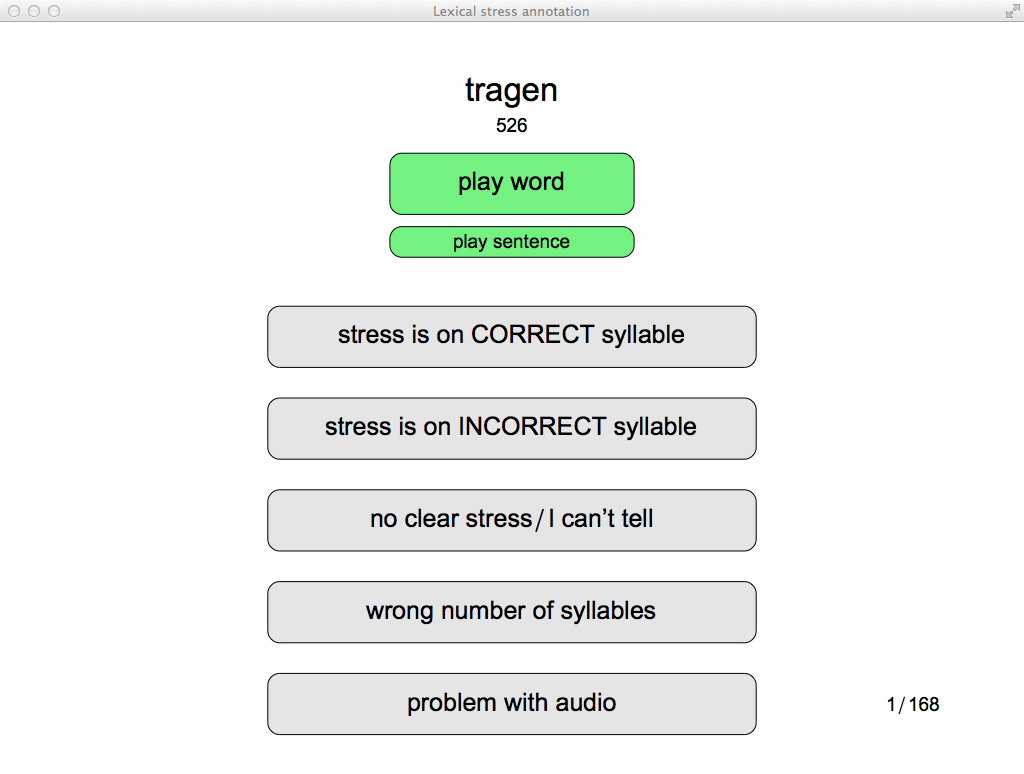
\includegraphics[width=\textwidth]{img/screenshots/AnnotationTool}
			\caption[A screenshot of the graphical annotation tool scripted in Praat.]{A screenshot of the graphical annotation tool scripted in Praat. Green buttons allow the annotator to listen to  the word and sentence utterances. Gray buttons allow the annotator to record their judgment of stress accuracy; from top to bottom, the buttons correspond to the labels [correct], [incorrect], [none], [bad\_nsylls], and [bad\_audio].}
			\label{fig:annotationtool}
		\end{figure}
		
		
		%\vspace{2em}
		
		The lexical stress error 
		annotations collected in this manner for each token (utterance) in the dataset enable two important contributions of this thesis, described in the following sections. 
		First, the multiple annotations for each token from different annotators permit an analysis of inter-annotator agreement with regard to the identification of lexical stress errors; \cref{sec:lexstress:agreement} presents this analysis, along with statistics on the relative frequencies with which the five labels were selected by annotators from the different L1 and expertise groups described in \cref{sec:lexstress:annotators}.
		Secondly, and perhaps more importantly, the errors identified by these annotators in the data extracted from the IFCASL corpus enable an analysis of the frequency of lexical stress errors in the speech of L1 French learners of German as L2; this is the subject of \cref{sec:lexstress:results}.
		
	
	\section{Inter-annotator agreement}
	\label{sec:lexstress:agreement}	
	
	To create a useful CAPT system for lexical stress errors in nonnative German, i.e. to automatically detect whether a student has made a lexical stress error in a given utterance, it is helpful to have an understanding of the difficulty of the error-detection task, not only for machines but for humans. It is therefore useful to analyze the collected stress accuracy judgments in terms of inter-annotator agreement, in order to gain insight into the nature of the challenge this task presents. If it is uncommon for human annotators to agree about whether a given lexical stress realization is correct or incorrect, this may indicate that  identifying lexical stress errors is a challenging task, and one which an automatic system should also be expected to have difficulty with. If, on the other hand, human annotators are generally in strong agreement, this may reflect a lower level of difficulty, and give reason to judge the performance of an automatic system by a higher standard.  
	
	As stated in the previous section,
	%\cref{sec:lexstress:data}, 
	lexical stress realizations in a total of 
	%669 
	668 word utterances were each assigned to one of five classes by multiple annotators, based on whether the annotator judged the production to have correctly placed stress, incorrectly placed stress, no clear stress placement, or other problems which prevented the annotator from making a judgment about the lexical stress accuracy. 
	For 268 of these utterances, i.e. approximately 40\% of the dataset, there was perfect agreement among annotators as to which of the five possible labels was most appropriate. This means that for the majority of the dataset (400 utterances, or approximately 60\%), at least one annotator's judgment diverged from that of the other(s) who labeled the same utterance.
	
	
	To make sense of these differences,  
	%and obtain a clearer picture of inter-annotator agreement in the error-detection task, the agreement between these judgments 
	agreement in label assignments was calculated for each pair of annotators who overlapped, i.e. labeled any of the same tokens. 
	%TODO {matrix of pairwise tokens in common (or just x/o to show which annotators overlapped?}
	%This section describes how this agreement was calculated, and the following sections \cref{sec:agreement:overall, sec:agreement:native, sec:agreement:expertise} present an analysis of the resulting inter-annotator agreement statistics. Finally, 
		Two metrics were used to quantify agreement between a pair of annotators: the simple percentage of observed agreement, and Cohen's Kappa ($\kappa$) statistic; the following paragraphs describe how these are computed. In the analysis presented in \cref{sec:agreement:overall,sec:agreement:native,sec:agreement:expert}, both metrics are presented together in the hopes of providing a more comprehensive picture of inter-annotator agreement than either can convey alone.  
		
		
		For a given pair of annotators, percentage agreement is calculated as the number of tokens to which both annotators assigned the same label, divided by the total number of tokens labeled by both annotators. Possible values for percentage agreement range from 0\%, representing complete disagreement between annotators, to 100\%, representing complete agreement. This simple metric ignores the probability of annotators agreeing by chance, and therefore may give a somewhat optimistic picture of inter-annotator agreement, but nevertheless serves as a basic, easy-to-interpret preliminary indication of the reliability of the collected judgments.
		
		To account for chance agreements not captured by the simple percentage of agreement, a second, more robust measure of inter-annotator agreement, Cohen's $\kappa$ statistic \citep{Cohen1960}, was also calculated for each pair of annotators. For a given pair of annotators who have labeled the same tokens, $\kappa$ is computed as
		\[
		\kappa = \frac{p_a-p_c}{1-p_c}
		\]
		where $p_a$ is the proportion of tokens assigned the same label by both annotators (i.e. the simple percentage agreement just described) and $p_c$ is the proportion of tokens which can be expected to receive the same label from both annotators purely by chance. The latter thus represents the probability of the two annotators agreeing by chance, and is calculated for a pair of annotators $A$ and $B$ as
		\[
		p_c = \sum_{s \in S} p_A(s) \times p_B(s)
		\]
		where $s$ is one of the stress judgments in the set of possible labels $S$:
		\[S = \{\text{[correct]}, \text{[incorrect]}, \text{[none]}, \text{[bad\_nsylls]}, \text{[bad\_audio]}\}\]
		and $p_A(s)$ is the proportion of tokens assigned the label $s$ by annotator $A$, calculated as the number of tokens assigned label $s$ by annotator $A$ divided by the total number of tokens labeled by annotator $A$; $p_B(s)$ is calculated in the same way for annotator $B$.
		%and $p_A(s)$ and $p_B(s)$ are the proportion of tokens assigned the label $s$ by annotators $A$ and $B$, respectively. The value of $p_A(s)$ is calculated as the number of tokens assigned label $s$ by annotator $A$ divided by the total number of tokens labeled by annotator $A$. 
		As $\kappa$ thus accounts for the probability of two annotators assigning a token the same label purely by chance, it provides a more conservative measure of inter-annotator agreement. A $\kappa$ value of 0 indicates that the annotators do not agree any more than would be expected by chance. If agreement between annotators is less than chance, $\kappa$ will take a value below 0. The maximum possible value of $\kappa$ is 1.00, which indicates perfect agreement between annotators.
		

		%\TODO{Anything else to say here?}
		
		\subsection{Overall agreement}
		\label{sec:agreement:overall}
		
		To obtain an overall measure of inter-annotator agreement for this lexical stress assessment task, the agreement between each pair of overlapping annotators was quantified by the metrics discussed in the previous section, and the minimum, median, mean, and maximum values over all pairwise comparisons were computed; these values are given in \cref{tab:agreement:overall}.
	Though this provides a rather coarse-grained picture of the overall agreement, this simple analysis already points to a few interesting observations. First of all, the mean and median percentage agreement are near 55\%, indicating that, roughly speaking, annotators agree just slightly more often than they disagree.
	%The $\kappa$ values are somewhat more difficult to interpret, but i
	Turning to the $\kappa$ values, given that $\kappa = 0$ represents agreement purely by chance while $k = 1$ represents perfect, meaningful agreement, the fact that the mean and median $\kappa$ values between annotators are somewhere near 0.25 indicates that the agreement observed between annotators is closer to what would be expected simply by chance than to agreement that would indicate highly reliable annotations, and signifies ``fair'' agreement between annotators according to the thresholds proposed by \textcite{Landis1977}. Examination of the minimum and maximum values reveals that while some pairs of annotators seem to exhibit ``substantial'' agreement, 
	%removing this because it's not certain that these numbers correspond to the same pair:
	%with one pair reaching over 80\% agreement and a $\kappa$ over 0.6, 
	indicating reasonably reliable judgments, other pairs have ``poor'' agreement; in one case, with 23.21\% agreement, the annotators seem to be closer to perfect disagreement than perfect agreement, and the corresponding $\kappa$ being below zero indicates that they agreed even (slightly) less than one would expect if they were merely labeling utterances randomly. 
	
	
	

		\begin{table}[b]
			\centering
			\caption{Overall pairwise agreement between annotators}
			\begin{tabular}{lrr}
			\toprule
				&	\% Agreement	&	Cohen's $\kappa$	\\
			\midrule
Mean		&	54.92\%	&	0.23	\\
Maximum	&	83.93\%	&	0.61	\\
Median		&	55.36\%	&	0.26	\\
Minimum	&	23.21\%	&	-0.01	\\
			\bottomrule
			\end{tabular}						
			
%			\begin{tabular}{lrrrr}
%				\toprule
%				Agreement measure &	Minimum	& Median &	 Maximum &	 Mean\\
%				\midrule
%				Percentage agreement &	23.21\%	& 55.36\%	& 83.93\%	& 54.92\% \\
%				Cohen's $\kappa$ & 	-0.01	& 0.26	& 0.61	& 0.23 \\
%				\bottomrule
%			\end{tabular}
			\label{tab:agreement:overall}
		\end{table}
	
		%%%%%% ANNOTATORS
	
	It seems, then, that there may be stark differences in reliability from annotator to annotator. Analysis of the set of pairwise comparisons between a given annotator and all overlapping annotators provides more insight into that annotator's individual reliability. 
	\Cref{fig:agreement:annotators} illustrates the pairwise agreements involving each of the 15 annotators, listed in \cref{tab:agreement:annotators}.
	 %\TODO{table of percent/kappa min/avg/max by annotator, since graphs are difficult to read precisely?} 
	 Evidently, there is noticeable variation from annotator to annotator, with some annotators (e.g. C, with a mean percentage agreement of 65.5\% and a mean $\kappa$ of 0.39) appearing generally more reliable than others (e.g. F, with mean \%=41.2\% and mean $\kappa$=0.13).  
	 %\TODO{stat. significance?} 
	 However, these figures should be interpreted with caution because they do not account for differences in the number of overlapping annotators/tokens available for each annotator. %TODO {reference overlap table}. 
	Nonetheless, the observed variability among annotators cannot be ignored, and \cref{sec:agreement:native,sec:agreement:expert} attempt to investigate whether differences in annotators' L1 and level of expertise could potentially explain some of this variability.
		
		
		\begin{table}[p]
			\centering
			\caption[Pairwise agreement statistics by annotator]{Pairwise agreement statistics by annotator. The number of pairwise comparisons (pairs) available for each annotator is listed, along with the minimum, mean, and maximum values across all pairs for that annotator.}
			
			\begin{tabularx}{\textwidth}{XXXXXXXX}			
			\toprule

\multirow{2}{*}{ID}	&	\multirow{2}{*}{Pairs}	&	\multicolumn{3}{c}{Pairwise \% Agreement}					&	\multicolumn{3}{c}{Pairwise $\kappa$}					\\
				\cmidrule(lr){3-5}						\cmidrule(lr){6-8}					
	&		&	Min.	&	Mean	&	Max.	&	Min.	&	Mean&	Max.	\\
\midrule															
A	&	8	&	23.2\%	&	51.4\%	&	67.3\%	&	-0.01	&	0.22	&	0.34	\\
B	&	7	&	48.2\%	&	62.4\%	&	80.4\%	&	0.17	&	0.33	&	0.61	\\
C	&	7	&	57.1\%	&	65.4\%	&	75.0\%	&	0.28	&	0.39	&	0.54	\\
D	&	7	&	42.9\%	&	52.0\%	&	63.2\%	&	0.22	&	0.29	&	0.47	\\
E	&	6	&	33.9\%	&	54.7\%	&	65.2\%	&	0.12	&	0.22	&	0.36	\\
F	&	7	&	28.6\%	&	41.2\%	&	55.4\%	&	0.04	&	0.13	&	0.25	\\
G	&	4	&	40.0\%	&	47.0\%	&	63.2\%	&	0.10	&	0.23	&	0.47	\\
H	&	7	&	38.4\%	&	66.9\%	&	83.9\%	&	0.13	&	0.29	&	0.47	\\
I	&	7	&	35.7\%	&	57.4\%	&	80.4\%	&	0.13	&	0.33	&	0.61	\\
J	&	7	&	39.3\%	&	58.3\%	&	73.2\%	&	0.11	&	0.20	&	0.32	\\
K	&	10	&	40.0\%	&	57.4\%	&	75.0\%	&	0.10	&	0.31	&	0.51	\\
L	&	8	&	39.3\%	&	57.4\%	&	75.0\%	&	0.08	&	0.30	&	0.54	\\
M	&	8	&	28.6\%	&	55.6\%	&	83.9\%	&	0.04	&	0.26	&	0.51	\\
N	&	7	&	23.2\%	&	43.0\%	&	69.6\%	&	-0.01	&	0.13	&	0.22	\\
O	&	6	&	40.5\%	&	47.4\%	&	53.6\%	&	0.13	&	0.20	&	0.28	\\		
			
			\bottomrule
			\end{tabularx}
			
			\label{tab:agreement:annotators}
		\end{table}
		
		\begin{figure}[p]
			\centering
			
			\begin{subfigure}{\textwidth}
				\centering
				\caption{Pairwise percentage agreement by annotator}
				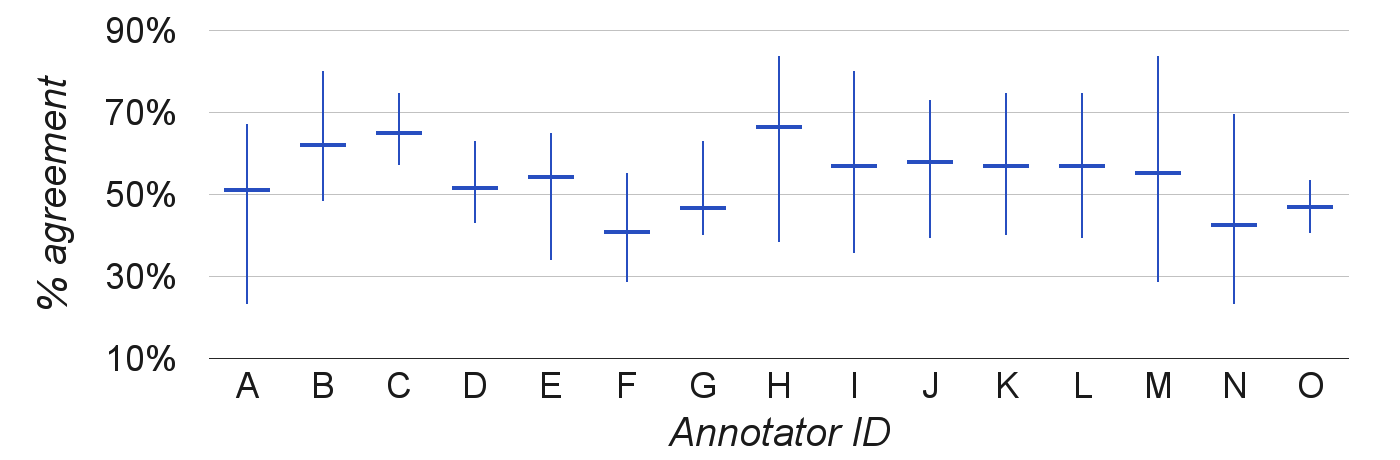
\includegraphics[width=\textwidth]{img/annotation/pairAgreeAnnotators-noTitle}
%				\caption{Percent agreement}
				\label{fig:agreement:annotators:pct}
			\end{subfigure}%

			%\vspace{1em}			
			
			\begin{subfigure}{\textwidth}
				\centering
				\caption{Pairwise $\kappa$ by annotator}
				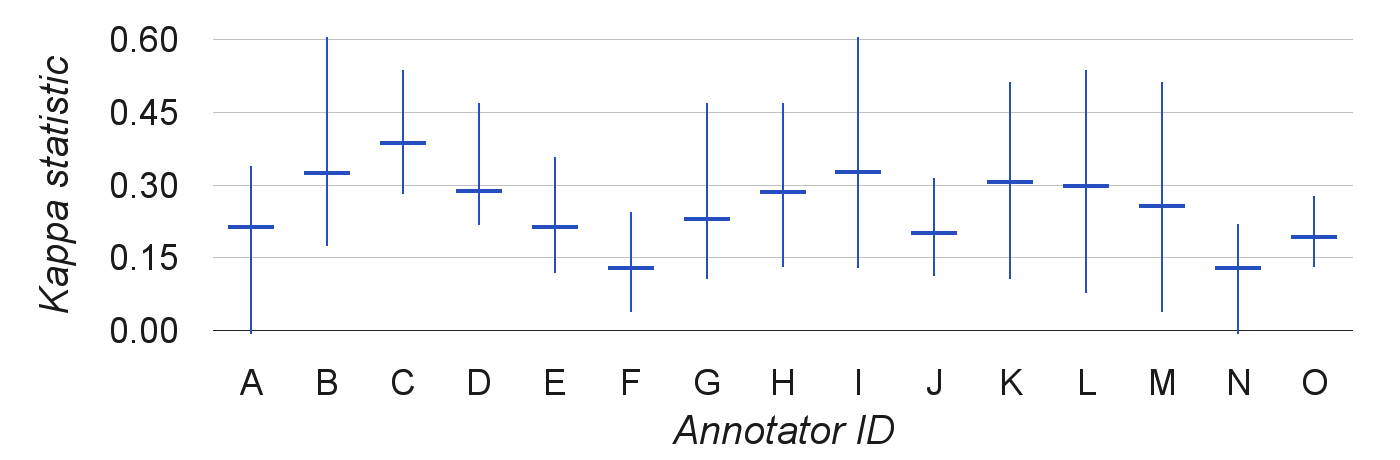
\includegraphics[width=\textwidth]{img/annotation/pairKappaAnnotators-noTitle}
%				\caption{Cohen's Kappa statistic}
				\label{fig:agreement:annotators:k}
			\end{subfigure}%			
			
			%\vspace{1em}			
			
			\caption[Pairwise agreement statistics by annotator]{Pairwise agreement statistics by annotator. The bottom of each vertical bar represents the minimum pairwise value, the top the maximum. Horizontal bars indicate mean pairwise values.}
			\label{fig:agreement:annotators}
		\end{figure}
		
%		\begin{figure}[p]
%			\centering
%			
%			\begin{subfigure}{\textwidth}
%				\centering
%				\caption{Pairwise percentage agreement by annotator}
%				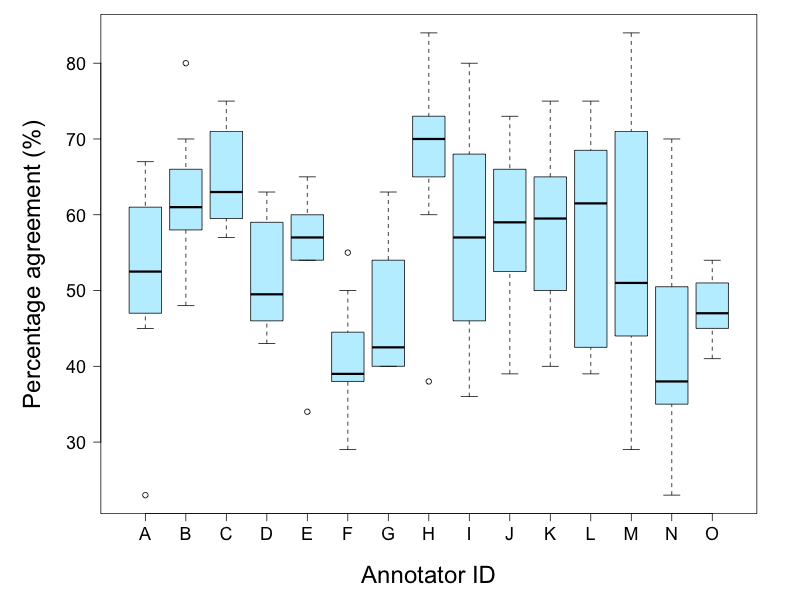
\includegraphics[width=\textwidth]{img/plots/pairwisePercentageByAnnotator-noTitle}
%				\label{fig:agreement:annotators:pct}
%			\end{subfigure}%
%
%			\vspace{1em}			
%			
%			\begin{subfigure}{\textwidth}
%				\centering
%				\caption{Pairwise $\kappa$ by annotator}
%				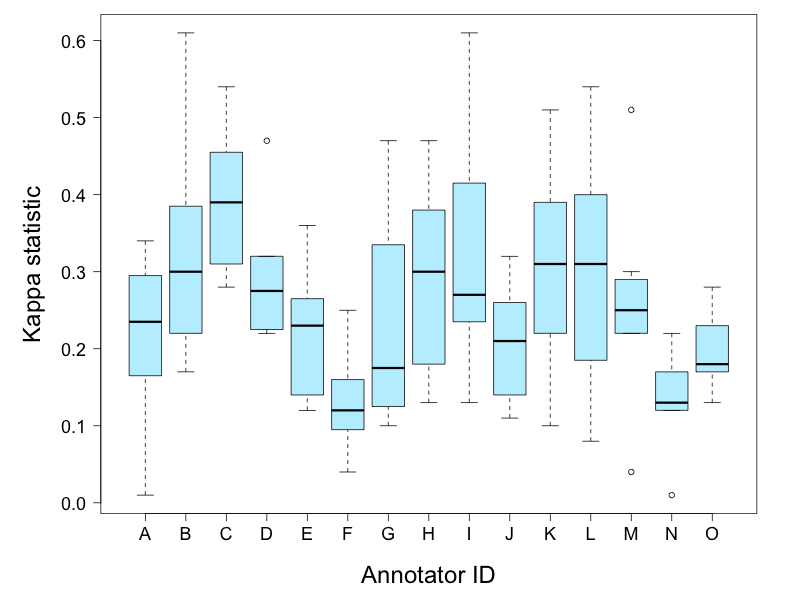
\includegraphics[width=\textwidth]{img/plots/pairwiseKappaByAnnotator-noTitle}
%				\label{fig:agreement:annotators:k}
%			\end{subfigure}%
%			
%			%\vspace{1em}	
%
%			\caption[Pairwise agreement statistics by annotator]{
%			\TODO{Redo: smaller height, bigger labels, diff box styles to show L1/expertise of each annotator?} 
%			Each annotator's pairwise agreement with all other annotators with whom they overlapped.
%			In these box-and-whisker plots, black horizontal lines represent median values, and boxes extend from the first quartile to the third quartile, thus representing the Inter Quartile Range (IQR). Whiskers (dashed lines) extend to the minimum and maximum values within 1.58 IQR of the first and third quartiles, respectively, and roughly represent a 95\% confidence interval around the median. 
%			 Circles depict outlying values that fall outside of the IQR by a distance of more than approximately 1.5$\times$IQR.%
%			%Numbers in parentheses indicate the number of pairwise comparisons involving each annotator. The bottom of each vertical bar represents the minimum pairwise value, the top the maximum. Horizontal bars indicate mean pairwise values.
%			
%			}
%			
%			\label{fig:agreement:annotators}
%		\end{figure}
		
		
		
		
		%%%%%% WORD TYPES
			
		It is also of interest to analyze the overall inter-annotator agreement for each word type in the dataset (see \cref{tab:bisyllwords} for the list of annotated word types). \TODO{table of  min/med/max/mean by word?} As \cref{fig:agreement:words} illustrates, there are noticeable differences in agreement among word types. Annotators exhibit relatively high agreement (``moderate'' according to \cite{Landis1977}) on certain words, such as \textit{E-mail}, \textit{halten}, and \textit{Pollen}), while for other words (e.g. \textit{manche} and \textit{Tschechen}) agreement values are closer to chance (``slight'' agreement in \citeauthor{Landis1977}'s schema). 
		No clear explanation for these variations readily presents itself, but one reasonable hypothesis might be that annotators may agree more often for words which are particularly easy or difficult for learners, i.e. words for which learners tend to make few/many errors, as a result of a high imbalance between correct and erroneous utterances. However, as the error distribution analysis in \cref{sec:results:wordtype} will show, this does not seem borne out by the data. The highest-agreement word types do not seem to have particularly imbalanced proportions of [correct] utterances; for \textit{E-mail}, \textit{halten}, and \textit{Pollen} approximately 60-65\% of utterances were [correct], which is close to the overall average of 63.77\%. Furthermore, some of the word types with unusually high or low proportions of [correct] utterances (e.g. \textit{Frühling}, with over 85\%, or \textit{Tatort}, with under 40\%), seem to have agreement relatively close to the overall average. Therefore, further work will be needed to shed light on whether the agreement differences observed among different word types might simply be a consequence of individual variation among the annotators assigned to each type, or whether other phenomena (e.g. frequency effects, segmental pronunciation errors, or interference from French) might be at play.
		
		\begin{table}%[p]
			\centering
			\caption[Pairwise agreement statistics by word type]{Pairwise agreement between annotators for each word type.  The number of pairwise comparisons (pairs) available for each word is listed, along with the minimum, mean, and maximum values across all pairs for that word.}
			
			\begin{tabularx}{\textwidth}{lXXXXXXX}			
			\toprule		

\multirow{2}{*}{Word type}	&	\multirow{2}{*}{Pairs}	&	\multicolumn{3}{c}{Pairwise \% Agreement}					&	\multicolumn{3}{c}{Pairwise $\kappa$}					\\
				\cmidrule(lr){3-5}						\cmidrule(lr){6-8}					
	&		&	Min.	&	Mean	&	Max.	&	Min.	&	Mean	&	Max.	\\
\midrule															
E-mail	&	3	&	57.1\%	&	66.1\%	&	75.0\%	&	0.34	&	0.45	&	0.54	\\
Flagge	&	10	&	32.7\%	&	50.9\%	&	67.3\%	&	0.10	&	0.24	&	0.47	\\
fliegen	&	6	&	37.5\%	&	56.6\%	&	73.2\%	&	0.12	&	0.23	&	0.38	\\
Frühling	&	6	&	28.6\%	&	55.1\%	&	83.9\%	&	0.04	&	0.18	&	0.30	\\
halten	&	6	&	57.1\%	&	67.9\%	&	80.4\%	&	0.28	&	0.42	&	0.61	\\
manche	&	3	&	41.1\%	&	44.1\%	&	46.4\%	&	0.10	&	0.14	&	0.19	\\
Mörder	&	6	&	46.4\%	&	55.4\%	&	67.9\%	&	0.12	&	0.20	&	0.38	\\
Pollen	&	6	&	58.5\%	&	67.1\%	&	76.8\%	&	0.32	&	0.42	&	0.56	\\
Ringen	&	6	&	42.9\%	&	47.1\%	&	50.9\%	&	0.22	&	0.24	&	0.28	\\
Tatort	&	6	&	37.5\%	&	52.7\%	&	69.6\%	&	0.04	&	0.22	&	0.45	\\
tragen	&	3	&	40.0\%	&	53.3\%	&	69.1\%	&	0.25	&	0.35	&	0.51	\\
Tscheschen	&	6	&	23.2\%	&	44.9\%	&	66.1\%	&	-0.01	&	0.14	&	0.27	\\		

			\bottomrule
			\end{tabularx}
			
			\label{tab:agreement:annotators}
		\end{table}
		
		
		\begin{figure}[p]
			\centering
			
			\begin{subfigure}{\textwidth}
				\centering
				\caption{Pairwise percentage agreement by word type}
				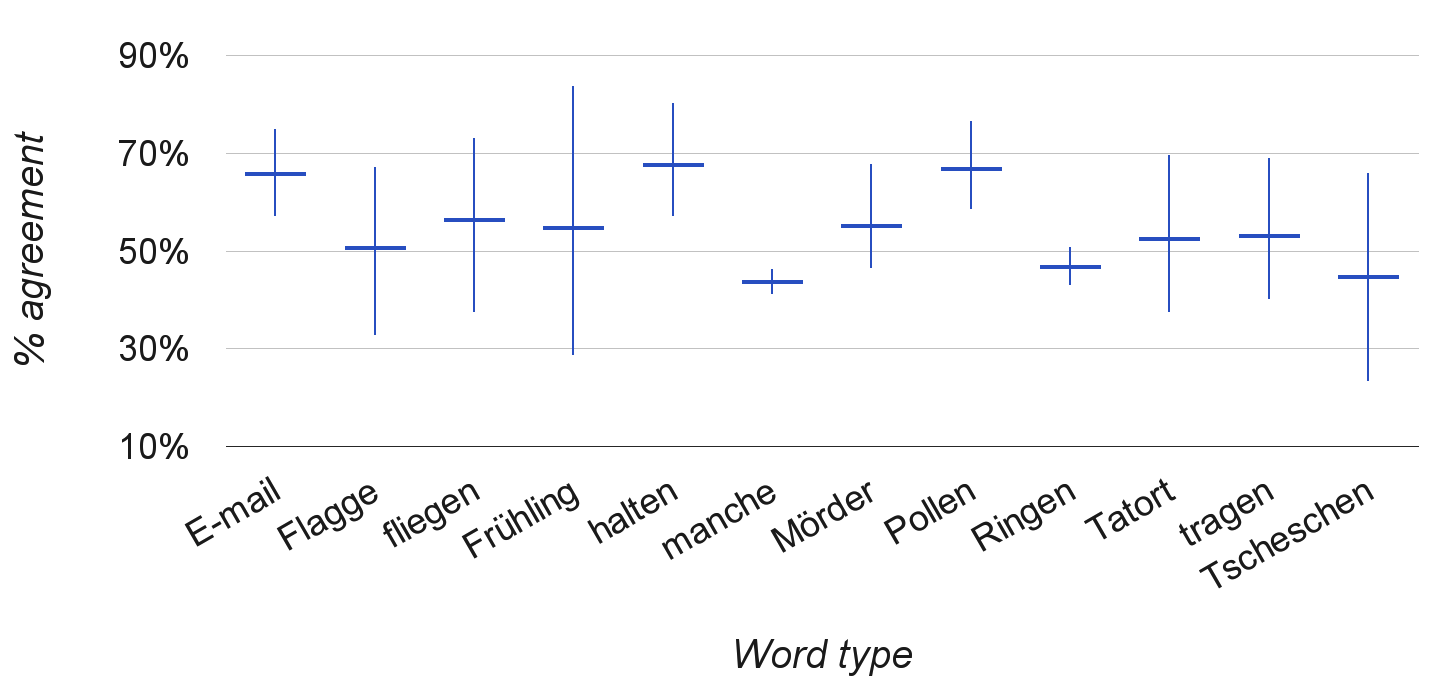
\includegraphics[width=\textwidth]{img/annotation/pairAgreeWords-noTitle2}
				\label{fig:agreement:words:pct}
			\end{subfigure}%
			
			\vspace{1.5em}
			
			\begin{subfigure}{\textwidth}
				\centering
				\caption{Pairwise $\kappa$ by word type}
				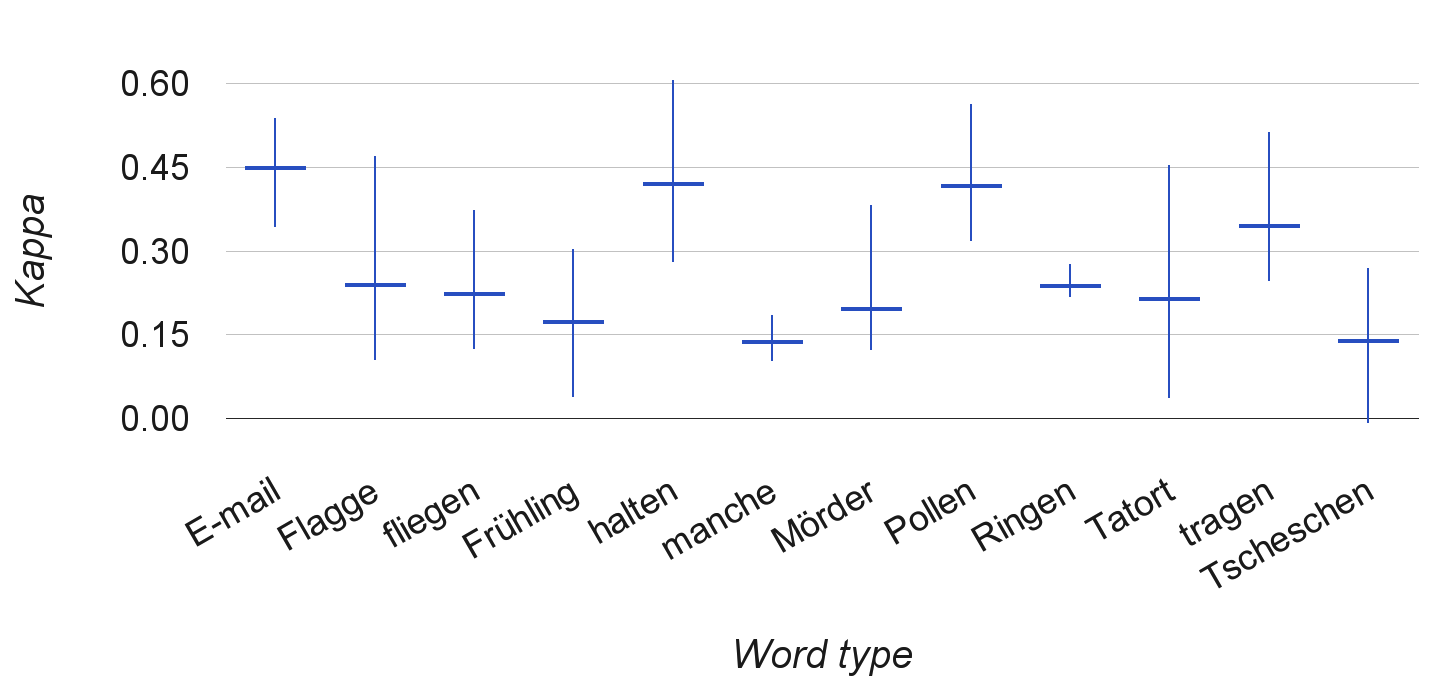
\includegraphics[width=\textwidth]{img/annotation/pairKappaWords-noTitle2}
				\label{fig:agreement:words:k}
			\end{subfigure}%
			
			\vspace{1.5em}
			
			\caption[Pairwise agreement statistics by word type]{Pairwise agreement between annotators for each word type. 
			The bottom of each vertical bar represents the minimum pairwise value, the top the maximum. Horizontal bars indicate average pairwise values.
			}
			\label{fig:agreement:words}
		\end{figure}				
		
		
%		\begin{figure}[phtb]
%			\centering
%							
%			
%			\begin{subfigure}{\textwidth}
%				\centering
%				\caption{Pairwise percentage agreement by word type}
%				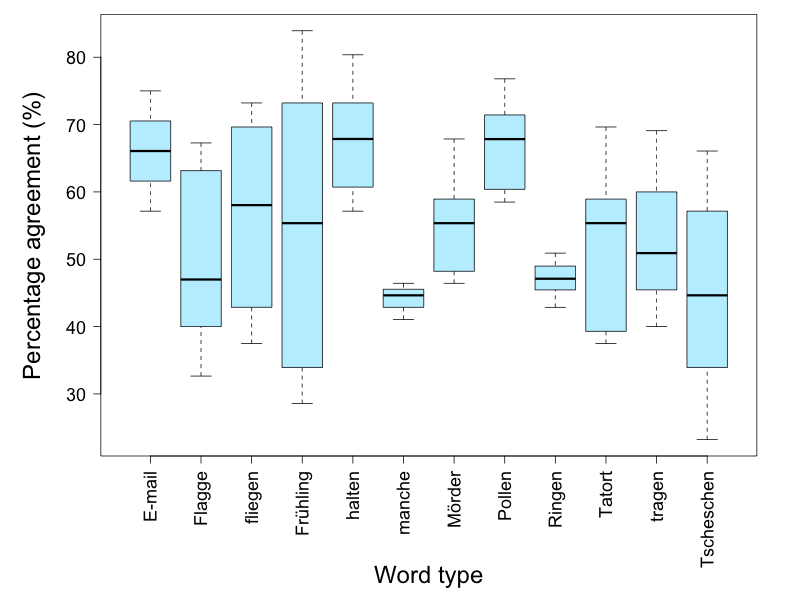
\includegraphics[width=\textwidth]{img/plots/pairwisePctByWord-noTitle}
%				\label{fig:agreement:words:pct}
%			\end{subfigure}%
%			
%			\vspace{1em}
%			
%			\begin{subfigure}{\textwidth}
%				\centering
%				\caption{Pairwise $\kappa$ by word type}
%				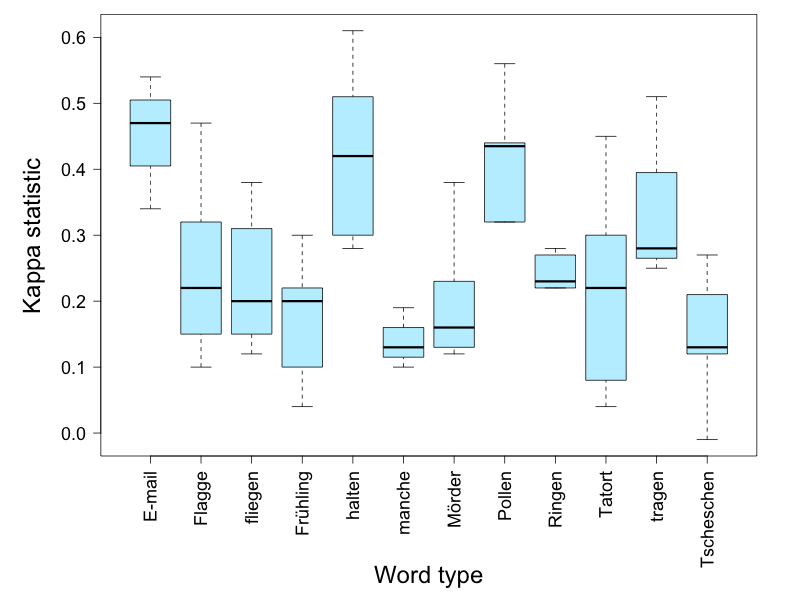
\includegraphics[width=\textwidth]{img/plots/pairwiseKappaByWord-noTitle}
%				\label{fig:agreement:words:k}
%			\end{subfigure}%
%			
%			%\vspace{1em}	
%			
%			
%			\caption[Pairwise agreement statistics by word type]{Pairwise agreement between annotators for each word type. 
%			See \cref{fig:agreement:annotators} on \cpageref{fig:agreement:annotators} for an explanation of the box-and-whisker plots displayed here.
%			%Horizontal lines represent median values. Colored boxes extend from the first quartile to the third quartile, and thus represent the Inter Quartile Range (IQR). Whiskers extend to the minimum and maximum values within 1.58 IQR of the first and third quartiles, respectively, and roughly represent a 95\% confidence interval around the median. Outliers that fall outside of the IQR by a distance of more than approximately 1.5$\times$IQR  are represented by circles.
%			%Numbers in parentheses indicate the number of pairwise comparisons available for each word type. The bottom of each vertical bar represents the minimum pairwise value, the top the maximum. Horizontal bars indicate average pairwise values.
%			}
%
%			
%			
%			\label{fig:agreement:words}
%		\end{figure}
		
		
		
		
	To put the agreement values reported in this section in context, it is worthwhile to compare them with those obtained in recent work by \textcite{Michaux2013} on L2 Dutch speech by L1 French speakers. In this study, three expert annotators were asked to indicate which
	 syllable they perceived as stressed in Dutch word utterances by the L1 French speakers. Two of the annotators were L1 Dutch speakers, the other an L1 French speaker who was nevertheless ``highly proficient'' in Dutch (p.~90). The authors report an average $\kappa$ of 0.71 between annotators, representing ``substantial'' agreement in the schema of \textcite{Landis1977}, and a much higher value than those observed in the present work. One plausible explanation for this difference may be the fact that while the three annotators participating in the \textcite{Michaux2013} study were all ``phonetically trained'' (p.~90), i.e. experts (see \cref{sec:lexstress:annotators}),
	the annotation project described here collected judgments from a larger number of annotators, and only two of the 15 participating annotators had extensive phonetic training. The relationship between annotator expertise and inter-annotator agreement is explored further in \cref{sec:agreement:expert}. 
		
			The following sections present detailed analyses of the agreement between annotators with different native languages (\cref{sec:agreement:native}) and different levels of expertise (\cref{sec:agreement:expert}).  However, on the whole, it already seems evident that inter-annotator agreement in this lexical stress error annotation task is relatively low. This may simply signal low reliability among the particular annotators participating in this study, but it may also be a preliminary indication of the considerable difficulty of the task of diagnosing errors in L1 French speakers' realizations of lexical stress in German; this notion will be revisited in \cref{sec:diag:classification}. 

	
	
		%\subsubsection{Native vs. nonnative annotators}
		%\subsection{Native vs. nonnative annotators}
		\subsection{Native vs. nonnative annotators}
		\label{sec:agreement:native}

		
		
		Going beyond the coarse-grained analysis of inter-annotator agreement described in the previous section, we come now to the second question raised at the beginning of this chapter:
		
		\textit{Are there differences in how native and nonnative German speakers identify errors?}
		
		%\TODO{expectations/speculations of what we will find?}
		
		To answer this question, it is useful to look at the inter-annotator agreement between native and nonnative annotators, as well as at the distribution of label types within each group. 
		
		\Cref{fig:agreement:L1} illustrates the inter-annotator agreement for all pairs in which one annotator was a native German speaker and the other a nonnative speaker, as well as agreement between pairs in which both annotators were native speakers. Due to the small size of the nonnative group (3 annotators) and the aforementioned technical problems with annotator G's data (see \cref{sec:lexstress:annotators}), there was very little overlap between nonnative annotators (only one pairwise comparison), preventing meaningful analysis of agreement within the nonnative group. The precise mean, maximum, median, and minimum pairwise values for the two agreement metrics are listed in \cref{tab:agreement:L1}, for both  native-nonnative pairs and native-native pairs. 
		
		Looking at these statistics, we see little difference between the two types of pairs; in particular, the mean percentage agreement and $\kappa$ values for native-nonnative and native-native pairs are quite close. 
		%\TODO{Stat significance?} 
		If anything, it would appear that agreement within the native annotator group is slightly lower and more varied than agreement between the native and nonnative groups, though this may be explained by the larger number of native-native pairs compared to native-nonnative. It would therefore seem that these agreement statistics do not tell us much about difference between how the two groups of annotators judge lexical stress accuracy.
		
		
		\begin{table}[p]%[tb]
			\centering
			\caption{Inter-annotator agreement between native and nonnative annotators (pairwise)}
			%\begin{tabularr}{\textwidth}{lXXXX}
			\begin{tabular}{lrrrr}
			\toprule
			& \multicolumn{2}{c}{Native vs. nonnative} & \multicolumn{2}{c}{Native vs. native} \\
			\cmidrule(lr){2-3} \cmidrule(lr){4-5}
			& \% Agreement & Cohen's $\kappa$ & \% Agreement & Cohen's $\kappa$  \\
			\midrule
Mean	&56.98\%	 & 0.29  & 53.87\%	& 0.25\\
Maximum&	76.79\%	& 0.56 & 83.93\%	 & 0.61\\
Median	& 57.14\%	 &0.25 &  50.91\%	& 0.23 \\
Minimum	&32.65\%	 & 0.10 &  23.21\% &	-0.01\\
			\bottomrule
			\end{tabular}
			\label{tab:agreement:L1}
		\end{table} 
		

		\begin{figure}[p]
			\centering
			\begin{subfigure}{.7\textwidth}
				\centering
				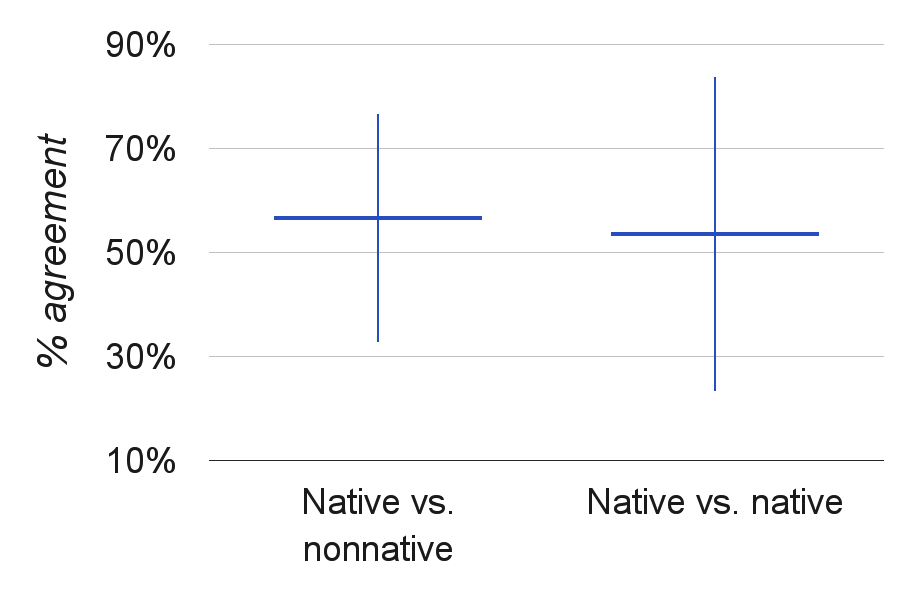
\includegraphics[width=\textwidth]{img/annotation/pairAgreeL1-noTitle}
				\caption{Pairwise \% agreement by L1 group}
				\label{fig:agreement:L1:pct}
			\end{subfigure}%

			\vspace{2em}			
			
			\begin{subfigure}{.7\textwidth}
				\centering
				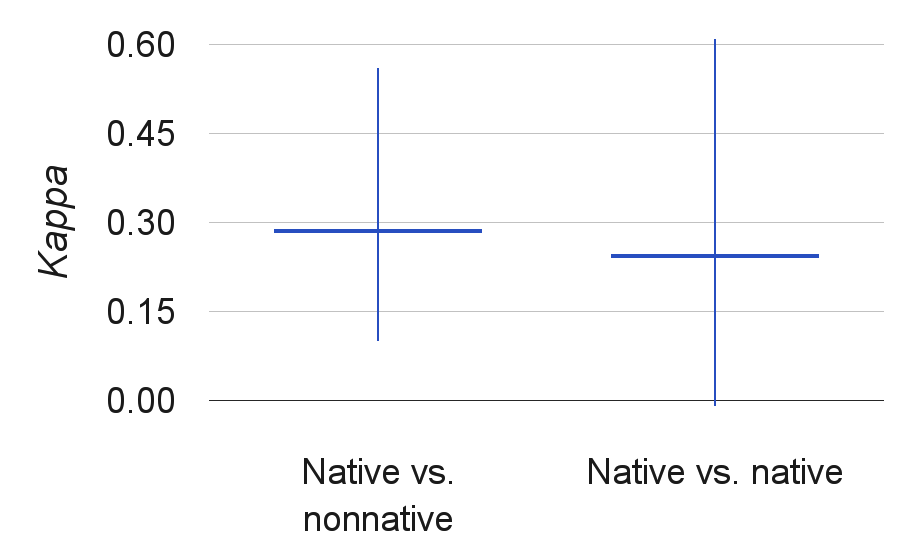
\includegraphics[width=\textwidth]{img/annotation/pairKappaL1-noTitle}
				\caption{Pairwise $\kappa$ by L1 group}
				\label{fig:agreement:L1:k}
			\end{subfigure}%		
			
			\vspace{1.5em}
			
			\caption[Pairwise agreement statistics by annotator L1 group]{Pairwise agreement between annotators based on L1 group (native or nonnative German speakers).
	The bottom of each vertical bar represents the minimum pairwise value, the top the maximum. Horizontal bars indicate average pairwise values.
			}
			\label{fig:agreement:L1}
		\end{figure}
		
		
%		\begin{figure}[h!]
%			\centering
%			
%			\begin{subfigure}{.5\textwidth}
%				\centering
%				\caption{Pairwise \% agreement by L1 group}
%				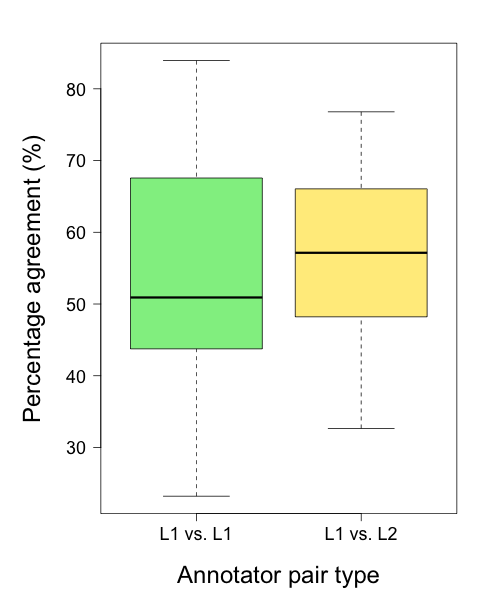
\includegraphics[width=\textwidth]{img/plots/pairwisePctByL1-noTitle}
%				\label{fig:agreement:L1:pct}
%			\end{subfigure}%
%			~
%			\begin{subfigure}{.5\textwidth}
%				\centering
%				\caption{Pairwise $\kappa$ by L1 group}
%				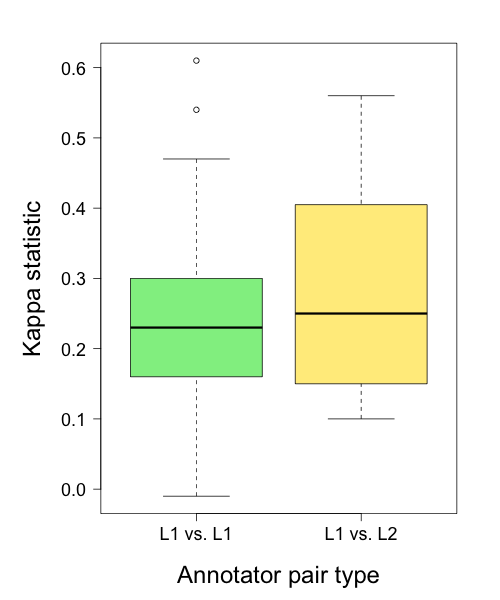
\includegraphics[width=\textwidth]{img/plots/pairwiseKappaByL1-noTitle}
%				\label{fig:agreement:L1:k}
%			\end{subfigure}%
%			
%			\caption[Pairwise agreement statistics by annotator L1 group]{\TODO{larger labels?} Pairwise agreement between annotators based on L1 group (L1 = native German speaker, L2 = nonnative speaker). 
%			See \cref{fig:agreement:annotators} on \cpageref{fig:agreement:annotators} for an explanation of the box-and-whisker plots displayed here.
%			%Horizontal lines represent median values. Colored boxes extend from the first quartile to the third quartile, and thus represent the Inter Quartile Range (IQR). Whiskers extend to the minimum and maximum values within 1.58 IQR of the first and third quartiles, respectively, and roughly represent a 95\% confidence interval around the median. Outliers that fall outside of the IQR by a distance of more than approximately 1.5$\times$IQR  are represented by circles.
%			%The bottom of each vertical bar represents the minimum pairwise value, the top the maximum. Horizontal bars indicate average pairwise values.
%			}
%			\label{fig:agreement:L1}
%		\end{figure}
		
		

		However, in comparing the relative frequencies of the different labels assigned by annotators in these two L1 groups, a more noticeable difference between the groups begin to emerge. As illustrated in \cref{fig:agreement:l1bars}, the native and nonnative speakers judged utterances as having correct lexical stress with approximately the same frequency: 52.7\% of native annotators' judgments were [correct], vs. 57.3\% for nonnative annotators. However, nonnative speakers seemed to choose the [none]
		%``no clear stress/I can't tell'' 
		label somewhat more frequently than native speakers (21.3\% vs. 11\%); this could indicate that nonnative speakers are less confident about how stress should be realized in German, resulting in less certainty about whether a given utterance is correct or not. 
		
		
			\begin{figure}[tb]
				\centering
				\caption[Distribution of labels by annotator L1]{Distribution of labels assigned by native and nonnative annotators,
				as a percentage of the total number of utterances labeled by that annotator group %\TODO{add exact values?}
				}
				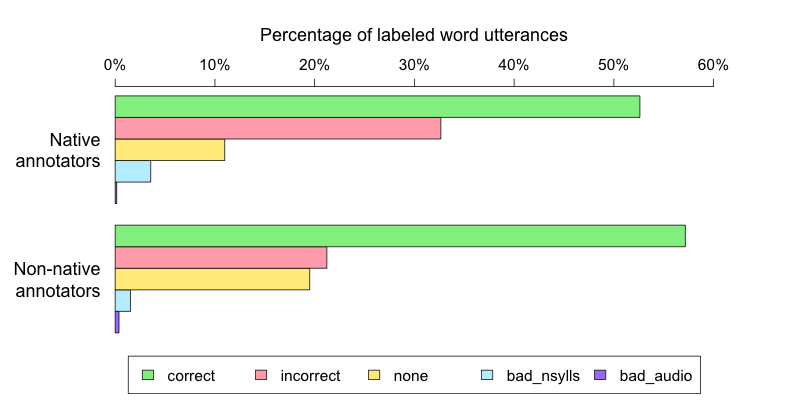
\includegraphics[width=\textwidth]{img/plots/pctJudgmentsByL1-notStacked}
				\label{fig:agreement:l1bars}
			\end{figure}
			
%			\begin{figure}[htb]
%				\centering
%				\caption{Stress judgments by native and nonnative annotators}
%				\includegraphics[width=.9\textwidth]{img/plots/pctJudgmentsByL1-NoTitle}
%				\label{fig:agreement:l1bars}
%			\end{figure}
	
%			\begin{figure}[htb]
%				\centering
%				\begin{subfigure}[b]{.5\textwidth}
%					\centering
%					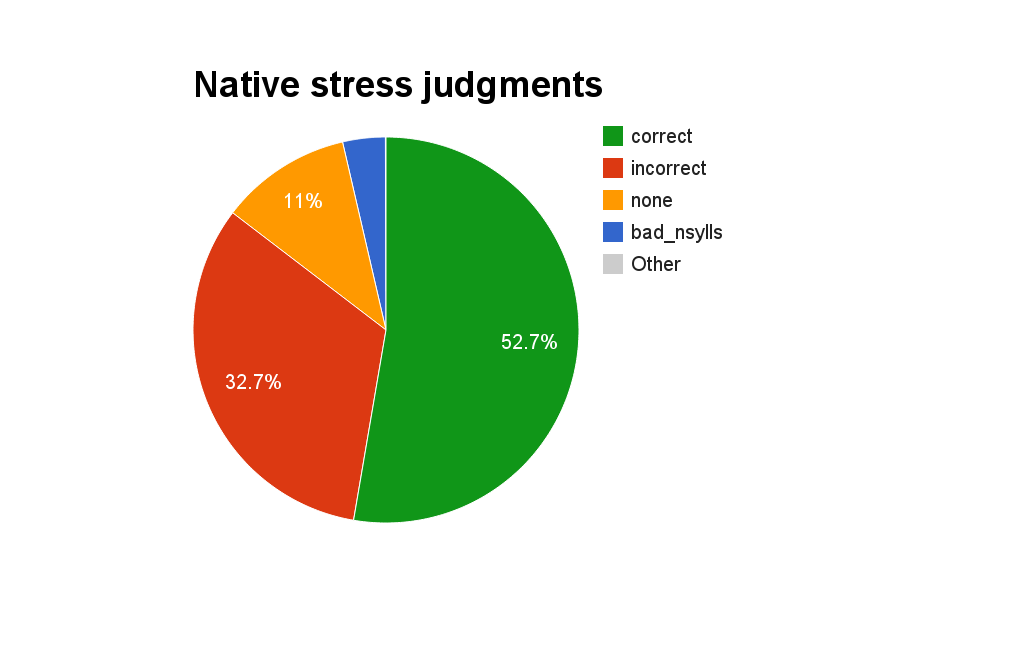
\includegraphics[width=\textwidth]{img/annotation/nativePie}
%					\caption{Native annotators}
%					\label{fig:l1pies:native}
%				\end{subfigure}%
%				~
%				\begin{subfigure}[b]{.5\textwidth}
%					\centering
%					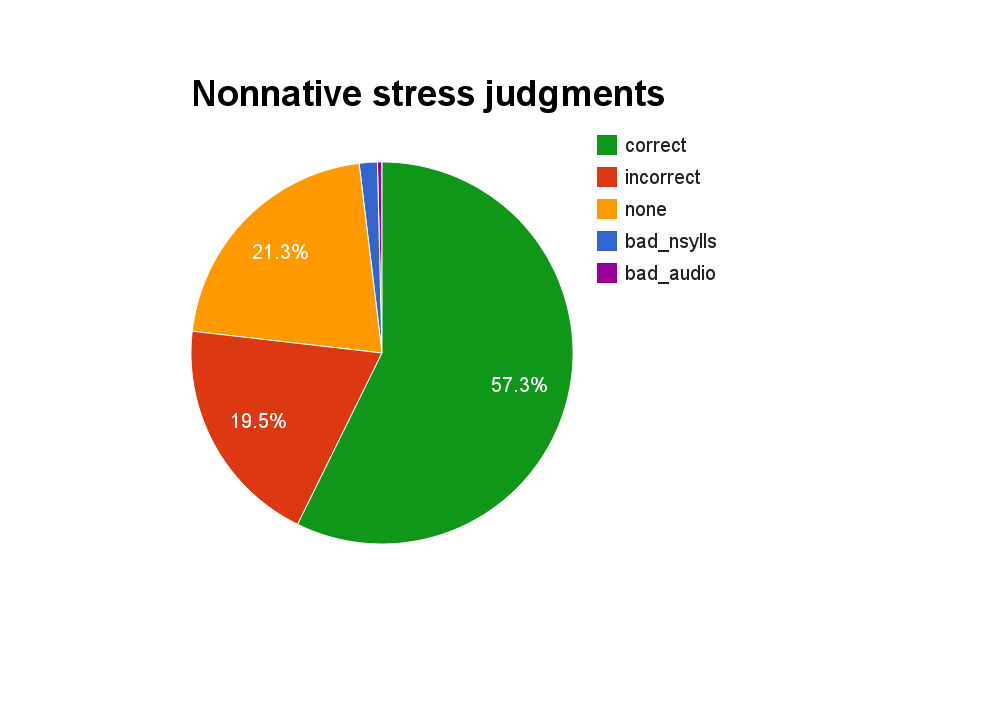
\includegraphics[width=\textwidth]{img/annotation/nonnativePie}
%					\caption{Nonnative annotators}
%					\label{fig:l1pies:nonnative}
%				\end{subfigure}%
%				\caption{Stress judgments made by native and nonnative German speakers}
%				\label{fig:l1pies}
%			\end{figure}
			
		Though the differences between native and nonnative annotators are interesting from the perspective of L2 perception of lexical stress, the ultimate goal of this thesis project is to create a CAPT tool which will help L1 French speakers be more intelligible when speaking German as L2, and therefore the way in which native German speakers perceive lexical stress in nonnative speech is of more relevance to this work than the way it is perceived by nonnative speakers. Therefore, the remainder of this chapter is concerned exclusively with the judgments of native annotators, which is to say that judgments by nonnative annotators are not included in the analyses that follow.
			
		
		\subsection{Expert vs. intermediate vs. novice annotators}
		\label{sec:agreement:expert}
		
		
		
	This section brings us to the last of the questions raised at the beginning of the chapter concerning inter-annotator agreement in the stress-annotated data, namely:
	
	\textit{Are there differences in how 
	%expert and novice annotators 
	annotators with different levels of expertise
	identify lexical stress errors?}
	
	Given the general difficulty of the task of identifying lexical stress errors, evidenced by relatively low overall inter-annotator agreement as discussed in \cref{sec:agreement:overall} above, it might seem reasonable to suppose that training in phonetics/phonology or experience annotating (nonnative) speech might have a positive impact on an annotator's ability to reliably judge the accuracy of lexical stress realizations by nonnative speakers. However, it once again bears mentioning that the ultimate goal of this work is to help L2 learners communicate intelligibly in German, and it can safely be assumed that in the vast majority of cases such learners will be communicating more often with native speakers who possess little formal knowledge of speech science than with expert phoneticians. Therefore, even if differences in reliability do exist between expert and novice annotators, it is important that the perception of nonnative lexical stress errors by non-experts not be ignored in favor of perception of such errors by experts. 
	
	%\TODO{mention that we're trying to train nonnative speakers to communicate in the L2, which means their speech will be ``evaluated'' by novices (native speakers), so we don't want to limit ourselves to expert judgments}

	%\TODO{Better transition needed here?}
	
	Just as the previous section analyzed native vs. nonnative annotations in terms of inter-annotator agreement and differences in label distributions between those groups, this section uses analogous data to investigate the differences between annotators of the three different expertise levels -- expert (exp.), intermediate (int.), and novice (nov.) -- described in \cref{sec:lexstress:annotators} above.
	
	To determine inter-annotator agreement between the three expertise groups, percentage agreement and $\kappa$ were tabulated for each pairing of annotators from different groups, i.e. for each of the following three pair types:
	%
	\begin{itemize}[topsep=-1em]
	\item{Expert annotator vs. novice annotator (Exp vs. Nov)}
	\item{Expert annotator vs. intermediate annotator (Exp vs. Int)}
	\item{Novice annotator vs. intermediate annotator (Nov vs. Int)}
	\end{itemize}
	%
	Additionally, pairwise agreement was tallied for pairings between two intermediate annotators (Int vs. Int), as a measure of inter-annotator agreement within this expertise group. Due to the small size of the expert and novice groups (two and three annotators, respectively), as well as the fact that expert annotators were deliberately not assigned overlapping tokens to label in an effort to maximize the number of tokens labeled by at least one expert,
	%\TODO{does that contradict the above statement about novice judgments being just as important as expert ones?}, 
	overlap within these groups was insufficient to calculate meaningful intra-group agreement statistics, so none are reported here. The small size of these two groups should also be kept in mind throughout the following analysis, as we should hesitate to draw firm conclusions from such small samples. 
		
		The agreement measures between groups and within the intermediate group are presented in \cref{tab:agreement:expertise} and illustrated in \cref{fig:agreement:expertise}. As these figures show, the mean values of both percentage agreement and $\kappa$ between the different expertise groups are quite close, and close to the overall means for all annotator pairs; 
		%\TODO{Stat significance?};  
		interestingly, the highest mean percentage agreement observed in this comparison (though only by a small margin) is that of expert-novice pairings, which might be a preliminary indication that there is no relevant difference in reliability between expertise levels. 
			
		
		
		\begin{table}[p]%[tb]
			\centering
			\caption[Pairwise agreement statistics by annotator expertise]{Pairwise agreement between annotators based on their level of expertise: expert (Exp), intermediate (Int), or novice (Nov).
			%{Pairwise agreement between expertise groups \TODO{explain abbreviations}
			}
			\begin{tabularx}{\textwidth}{lXXXXXXXX}
				\toprule
		& \multicolumn{2}{c}{Exp vs. Nov} & \multicolumn{2}{c}{Exp vs. Int} & \multicolumn{2}{c}{Nov vs. Int} & \multicolumn{2}{c}{Int vs. Int} \\
	&\% Agr.	& $\kappa$	&\% agr. &	$\kappa$&	\% agr.	& $\kappa$	&\% agr. & $\kappa$ \\
	\midrule
Mean	& 57.89\%	& 0.23	& 55.30\%	& 0.23	& 52.12\%	& 0.26	& 51.44\%	& 0.23 \\
Maximum	& 71.43\%	& 0.44	& 83.93\%	& 0.32	& 71.43\% & 	0.47	& 80.36\%	& 0.61 \\
Median	& 68.46\%	& 0.24	& 49.95\%	& 0.25	& 51.70\%	& 0.26	& 47.58\%	& 0.22\\
Minimum	& 23.21\%	& -0.01	& 33.93\%	& 0.10	& 35.71\%	& 0.08	& 28.57\%	&  0.04 \\
				\bottomrule
			\end{tabularx}
			\label{tab:agreement:expertise}
		\end{table}
			
			
		\begin{figure}[p]
			\centering

			\begin{subfigure}{.7\textwidth}
				\centering
				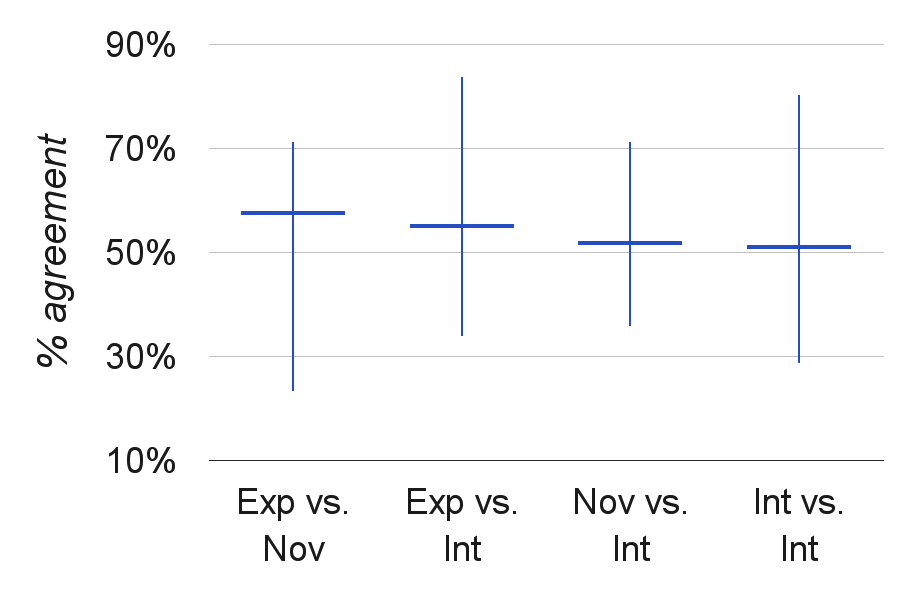
\includegraphics[width=\textwidth]{img/annotation/pairAgreeExpertise-noTitle}
				\caption{Pairwise \% agreement by expertise group}
				\label{fig:agreement:expertise:pct}
			\end{subfigure}%

			\vspace{2em}			
			
			\begin{subfigure}{.7\textwidth}
				\centering
				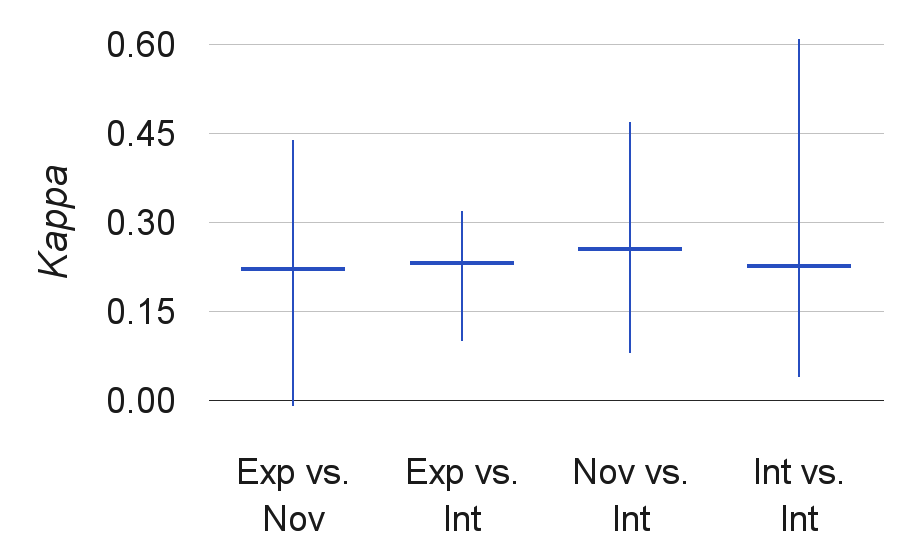
\includegraphics[width=\textwidth]{img/annotation/pairKappaExpertise-noTitle}
				\caption{Pairwise $\kappa$ by expertise group}
				\label{fig:agreement:expertise:k}
			\end{subfigure}%
			
			\vspace{1.5em}
					
			\caption[Pairwise agreement statistics by annotator expertise group]{Pairwise agreement between annotators based on their level of expertise: expert (Exp), intermediate (Int), or novice (Nov). 
			The bottom of each vertical bar represents the minimum pairwise value, the top the maximum. Horizontal bars indicate average pairwise values.
			}
			\label{fig:agreement:expertise}		

		\end{figure}
		
		
%		\begin{figure}[p]
%			\centering
%	
%			\begin{subfigure}{\textwidth}
%				\centering
%				\caption{Pairwise \% agreement by expertise group}
%				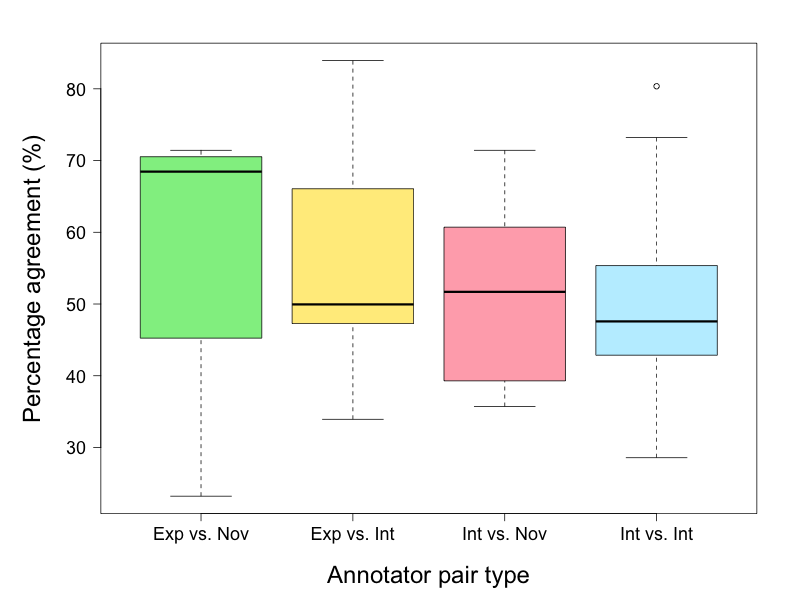
\includegraphics[width=\textwidth]{img/plots/pairwisePctByExpertise-noTitle}
%				\label{fig:agreement:expertise:pct}
%			\end{subfigure}%
%			
%			\vspace{1em}			
%			
%			\begin{subfigure}{\textwidth}
%				\centering
%				\caption{Pairwise $\kappa$ by expertise group}
%				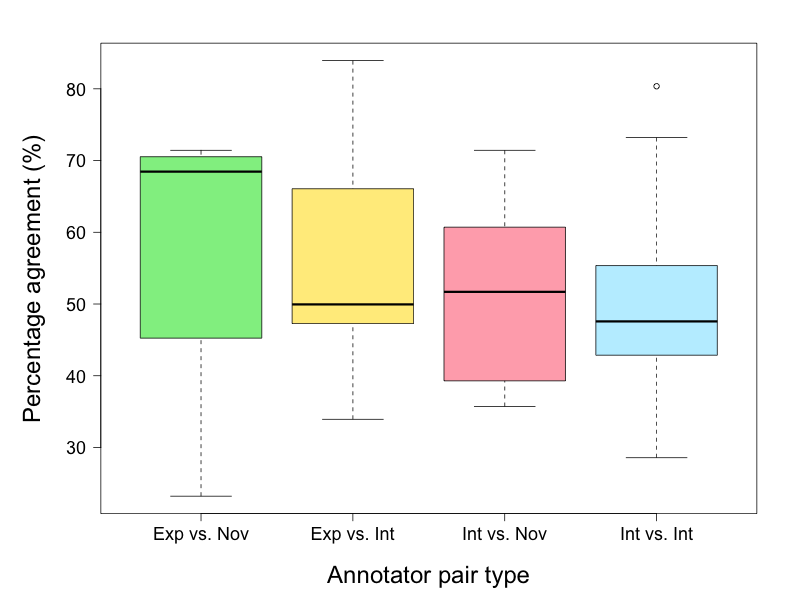
\includegraphics[width=\textwidth]{img/plots/pairwisePctByExpertise-noTitle}
%				\label{fig:agreement:expertise:k}
%			\end{subfigure}%
%			
%			\caption[Pairwise agreement statistics by annotator expertise]{Pairwise agreement between annotators based on their level of expertise: expert (Exp), intermediate (Int), or novice (Nov). 
%			See \cref{fig:agreement:annotators} on \cpageref{fig:agreement:annotators} for an explanation of the box-and-whisker plots displayed here.
%			%The bottom of each vertical bar represents the minimum pairwise value, the top the maximum. Horizontal bars indicate average pairwise values.
%			}
%			\label{fig:agreement:expertise}
%		\end{figure}
		
			\Cref{fig:agreement:expertisebars} illustrates the relative number of each label type as assigned by annotators of the three expertise levels described in \cref{sec:lexstress:annotators} above, and while any analysis of this data should bear in mind the small sample sizes of the expert and novice groups (two and three annotators, respectively), it does appear that some interesting differences may exist between the three groups. 
			
			Expert annotators seem to be far more ``generous'' in their labeling than intermediate or novice annotators, in that the experts assigned the [correct] label 73.6\% of the time, in contrast with 49.3\% and 54.8\% for the other two groups respectively. One could speculate that experts' familiarity with nonnative speech and knowledge of possible inter-speaker variations in lexical stress realization may be the cause for this willingness to accept a high proportion of utterances as correct. 
			
			Another interesting difference can be observed between the intermediate and novice annotator groups: compared with the intermediate annotators, novices assign the [none] label less frequently (5.8\% of the time, versus 16.3\% for intermediates) and the [bad\_nsylls] label more frequently (8.4\% of the time, versus 2.1\% for intermediates). Still keeping in mind the discrepancy in sample sizes when comparing 10 intermediate annotators to three novices, 
			%\TODO{we might} speculate
			it seems plausible that if experts' extensive experience with nonnative speech could be an explanation for their aforementioned ``generosity'' with the [correct] label, novice annotators' lack of experience with nonnative speech could in a similar way make them ``harsher'' in judging nonnative utterances as having an incorrect number of syllables. 
			
			\begin{figure}[tb]
				\centering
				\caption[Distribution of labels by annotator expertise]{Distribution of labels assigned by annotators of different expertise levels,
				as a percentage of the total number of utterances labeled by that annotator group
				}
				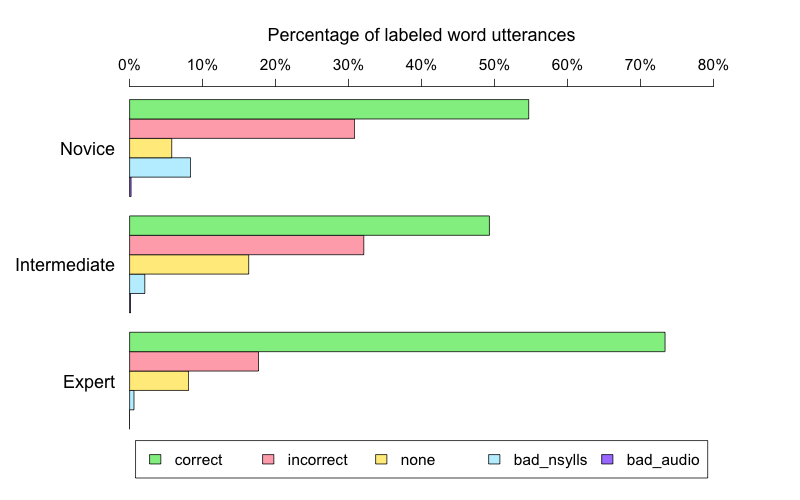
\includegraphics[width=\textwidth]{img/plots/pctJudgmentsByExpertise-notStacked}
				\label{fig:agreement:expertisebars}
			\end{figure}			
			
			
%			\begin{figure}[htb]
%				\centering
%				\caption{Stress judgments by annotator expertise}
%				\includegraphics[width=.9\textwidth]{img/plots/pctJudgmentsByExpertise-NoTitle}
%				\label{fig:agreement:expertisebars}
%			\end{figure}
			
%			\begin{figure}[htb]
%				\centering
%				\begin{subfigure}[b]{.5\textwidth}
%					\centering
%					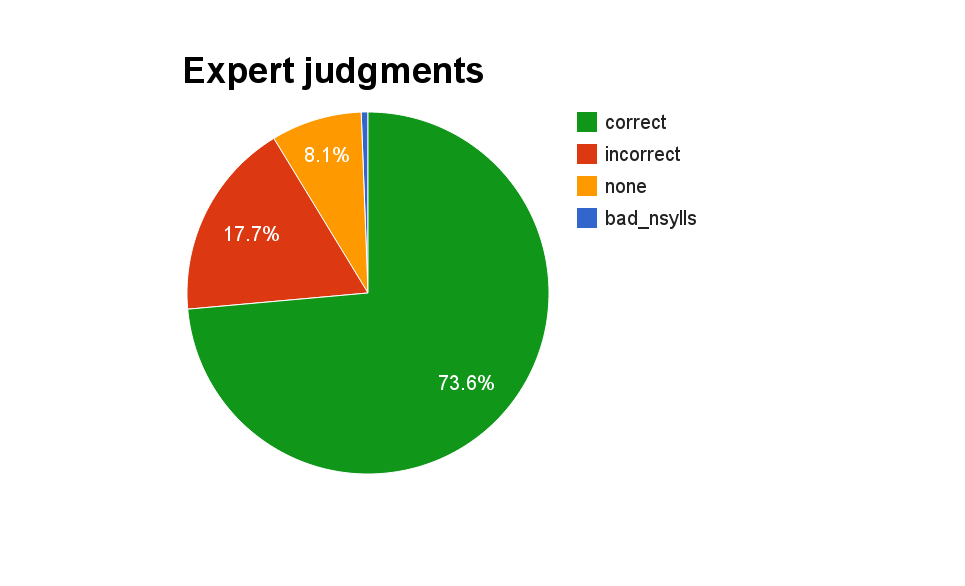
\includegraphics[width=\textwidth]{img/annotation/expertPie}
%					\caption{Expert}
%					\label{fig:expertisepies:expert}
%				\end{subfigure}%
%				
%				\begin{subfigure}[b]{.5\textwidth}
%					\centering
%					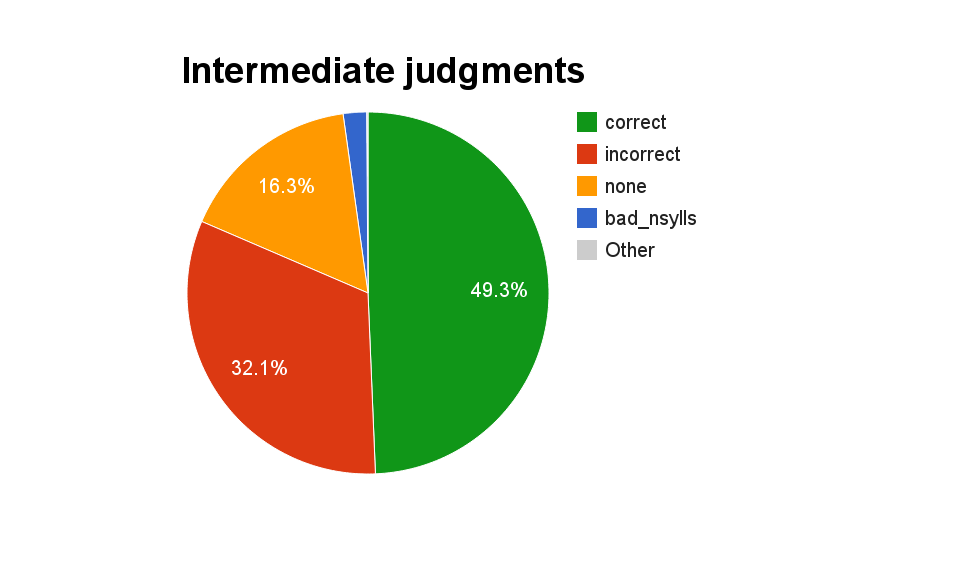
\includegraphics[width=\textwidth]{img/annotation/intermediatePie}
%					\caption{Intermediate}
%					\label{fig:expertisepies:intermediate}
%				\end{subfigure}%
%				~
%				\begin{subfigure}[b]{.5\textwidth}
%					\centering
%					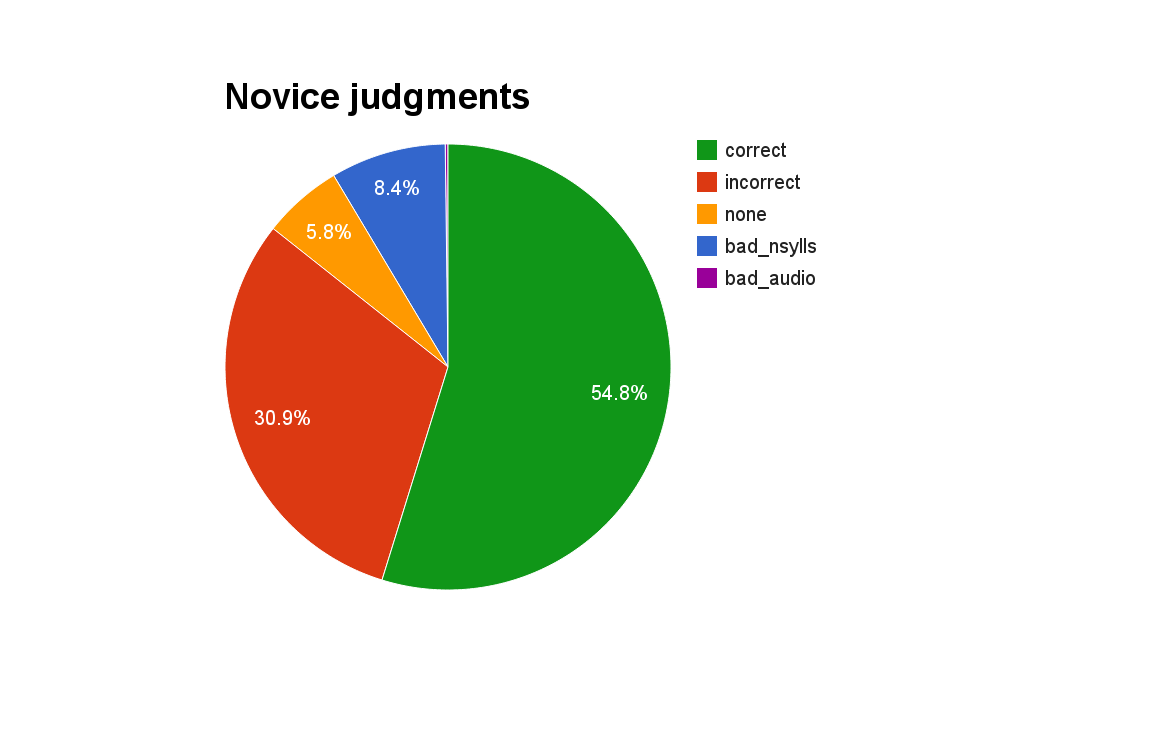
\includegraphics[width=\textwidth]{img/annotation/novicePie}
%					\caption{Novice}
%					\label{fig:expertisepies:novice}
%				\end{subfigure}%
%				\caption{Stress judgments by annotator expertise}
%				\label{fig:expertisepies}
%			\end{figure}
			
			
			
		\section{Choosing gold-standard labels}
		\label{sec:agreement:gold}
		
		
		
		As the previous sections have illustrated, having multiple annotators judge the accuracy of each lexical stress production was useful insofar as it led to some interesting observations about the difficulty of reliably assessing lexical stress accuracy, as well as insight into the differences in how judgments by annotators with different native languages and levels of expertise compare. However, if the annotations are to be used to analyze the distribution of errors in learner speech, or to train an automated error-diagnosis system (see \cref{sec:diag:classification}), each token in the dataset must ultimately be assigned a single ``gold-standard'' label from the set of possible labels (see \cref{sec:lexstress:method}), henceforth referred to as $S = \{$[correct],{[incorrect]},{[none]},{[bad\_nyslls]},{[bad\_audio]}$\}$.
		 In error analysis and classifier training, the gold-standard label will represent the ground truth as to whether a given utterance contains a lexical stress error.
		% which will be referred to henceforth as  $S$: $\{$[correct],{[incorrect]},{[none]},{[bad\_nyslls]},{[bad\_audio]}$\}$. 
		
		In some cases, assigning a gold-standard label was trivial, while in others a decision had to be made between competing candidate labels. This section describes the procedure by which a single label was chosen for each word token (utterance) in the data set described in \cref{sec:lexstress:data}. In the remainder of this section, the gold-standard label chosen for a given word token $t$ will be referred to as $s_{\text{gold}}(t)$.
		%, where $s$ stands for one of the possible labels, i.e. $s \in S$.
		
		To prepare for gold-standard labeling, all available annotations for $t$ were tallied by their label type $s \in S$, resulting in a set $S_t \subseteq S$ of labels assigned to $t$ by any of the native annotators who labeled this token (nonnative annotators' judgments were omitted as mentioned in \cref{sec:agreement:native} above). For each label $s(t) \in S_t$, the number of ``votes'' for that label was recorded as the number of annotators who assigned this label to token $t$,
		making it possible to determine which label(s) received the highest number of votes and may thus be considered the best candidate(s) for $s_{\text{gold}}(t)$. The set of highest-voted candidate labels will be referred to as $S_{t\text{-max}} \subseteq S_t$.
		%henceforth \TODO{\textit{need better notation for maxvotes set: }$S_{\text{max}} \subseteq S_t$} will refer to the set of labels for $t$ with the highest number of votes \TODO{reword?}.
		
		Given the observed labels and their vote counts, a rule-based procedure was followed to assign a gold-standard label $s_{\text{gold}}(t)$ to each token $t$ in the dataset; this procedure is outlined in \cref{tab:agreement:goldrules}. At each step $i$ in the procedure, any tokens whose set $S_t$ of observed labels fits condition $C_i$ are assigned the gold-standard label described in column $s_{\text{gold}}(t)$; the number of tokens matching $C_i$ is given as $N(C_i)$, and 
		% gives the number of tokens labeled at this step, i.e. the number matching $C_i$. The rightmost column 
		$N(C_{1 \dots i})$ represents the total number of tokens which have been assigned a gold-standard label at the end of step $i$ in the labeling procedure (i.e. the number of tokens matching $C_i$ or any previous condition).
		
		

		\begin{table}[tb]
		\centering
		\caption[Procedure for choosing a gold-standard label for a given token]{Procedure for choosing a gold-standard label $s_{\text{gold}}(t)$ for a given token $t$. At step $i$, tokens matching the condition $C_i$ are assigned the label in column $s_{\text{gold}}(t)$. The rightmost columns $N(C_i)$ and $N(C_{1 \dots i})$ list the number of tokens labeled in step $i$ and the total number that have been labeled at the end of step $i$, respectively.}
		
			\renewcommand{\arraystretch}{2}
			\begin{tabularx}{\textwidth}{rXlrr}
			\toprule
			Step ($i$)
			& Condition ($C_i$) 
			%\TODO{reword w/ $S_t$\&$S_{t\text{-max}}$} 
			& $s_{\text{gold}}(t)$ 
			& $N(C_i)$ 
			& $N(C_{1 \dots i})$ 
			\\
			\midrule
			
			1.& 
			$|S_t|=1$, i.e. $S_t = \{s_a\}$
			%$S_t = \{s_{\text{only}}\}$ (i.e. $|S_t|=1$)
			%There is only one label $s_{\text{only}}$ with any votes 
			& 
			$s_a$
			%$s_{\text{only}}$ 
			& 268 & 268 \\
			 
			2.& 
			$|S_{t\text{-max}}|=1$, i.e. $S_{t\text{-max}} = \{s_m\}$
			%One label $s_m$ has more votes than any other labels 
			& 
			%$s_{\text{gold}}(t) \gets 
			$s_m$ & 265 & 533 \\
			
			3.& 
			$s_{\text{exp}} \in S_{t\text{-max}}$
			%There is a label $s_{\text{exp}}$ assigned by an expert 
			& 
			%$s_{\text{gold}}(t) \gets 
			$s_{\text{exp}}$ & 51 & 584 \\
			
			4.& 
			$|S_{t\text{-max}}| = 2$, \mbox{[bad\_nsylls]} $\in S_{t\text{-max}}$,
			\newline
			i.e. $S_{t\text{-max}} = \{\text{[bad\_nsylls]}, s_o\}$	
			%\mbox{[bad\_nsylls]} is one of the competing labels, 
			%ignore it; \newline if 
			%and there is only one other competing label $s_{\text{only}}$  \TODO{reword}
			%remains 
			& 
			%$s_{\text{gold}}(t) \gets 
			$s_o$ & 17 & 601 \\
			
			5.& 
			$|S_{t\text{-max}}| = 3$
			%There is a three-way tie between labels
			%, indicating that the accuracy of the lexical stress realization is not clear 
			&
			% [correct], [none], and [incorrect] & 
			%$s_{\text{gold}}(t) \gets$ 
			\mbox{[none]} & 6 & 607\\
			
			6.& 
			$S_{t\text{-max}} = \{\text{[none]}, s_{\text{cert}}\}$, %with
			\newline
			%There are two competing labels: 
			%one of which is 
			%\mbox{[none]} and 
			%the other of which is 
			$s_{\text{cert}} \in \{$[correct],[incorrect]$\}$ 
			&
			$s_{\text{cert}}$ & 21 & 628\\
			
			7.& 
			$S_{t\text{-max}} = \{\text{[correct]},\text{[incorrect]}\}$
			%There are two competing labels: \mbox{[correct]} and \mbox{[incorrect]} 
			&
			\mbox{[correct]} & 40 & 668\\
	
			\bottomrule
			\end{tabularx}
			
		\label{tab:agreement:goldrules}
		\end{table}
		
				
		
		
		
		%1
		As mentioned in \cref{sec:agreement:overall}, for 268 of the 
		%669 
		668 tokens annotated, there was no disagreement whatsoever between annotators: for each of these 268 tokens, all annotators who labeled the token made the same judgment, making it easy to assign this label ($s_a$) as the gold standard for the utterance. Condition 1 ($C_1$) in \cref{tab:agreement:goldrules} captures this category of tokens. 
		%2
		For another 265 tokens, a majority of annotators assigned the same label, though one or more annotators dissented, so assigning the majority-vote label ($s_m$) as $s_{\text{gold}}(t)$ is logical; these are captured by $C_2$. 
		
		Therefore, for a total of 533 tokens (approximately 80\% of the word utterances in the dataset), the choice of $s_{\text{gold}}(t)$ was essentially uncontroversial.
		%
		For the remaining 
		%116 
		utterances, however, choosing gold-standard labels was a less straightforward task,
		and the decisions made in steps 3-7 are somewhat more controversial.
		
		%3
		In a third step, if either of the two expert annotators had labeled one of the remaining tokens, the expert's judgment ($s_{\text{exp}}$) was taken as $s_{\text{gold}}(t)$; 51 tokens met this condition ($C_3$). 
		
		%4
		Next, in step 4, if there were exactly two labels in $S_{t\text{-max}}$ and one of them was [bad\_nsylls], the other label ($s_o$) was chosen as $s_{\text{gold}}(t)$. The reasoning behind this step is that since the label [bad\_nsylls] was intended to be applied to utterances for which no stress judgment was possible, then if at least one annotator was able to make a judgment, the [bad\_nsylls] label must not be appropriate and should be rejected. This condition ($C_4$) applied to 17 tokens. 
		
		%5
		The following step (5) addressed tokens for which the set of competing labels $S_{t\text{-max}}$ had three members, i.e. for which there was a three-way tie between labels. The fact that so many different labels were assigned to each of these tokens was taken as an indication that the accuracy of the lexical stress realization in this utterance was quite difficult to judge, i.e. it is unclear which syllable in the uttered word has been stressed; as the label [none] is intended to capture such cases, this label was chosen as the gold standard for the 6 utterances matching this condition ($C_5$).
		
		%6
		The next condition ($C_6$) captured the 21 cases in which $S_{t\text{-max}}$ contained exactly two labels competing for gold-standard status, with one of the labels being [none] and the other being one of the two labels associated with certainty about the accuracy of the lexical stress realization, i.e. [correct] or [incorrect]. In these cases, [none] was rejected in favor of the certain label ($s_{\text{cert}}$), based on the assumption that if at least one annotator was able to categorically classify the given utterance as correctly or incorrectly realizing lexical stress, other native-speaking listeners might be inclined to make the same judgment. %\TODO{fix that sentence}.
		
		%7
		The remaining 40 utterances were captured by the seventh and final condition, $C_7$, in which $S_{t\text{-max}}$ contained exactly two labels: [correct] and [incorrect]. In these cases, the learner's utterance was assessed generously and the [correct] label was chosen as $s_{\text{gold}}(t)$, to capture the fact that as mentioned in \cref{sec:agreement:overall}, assessing the accuracy of a lexical stress realization seems to be a somewhat difficult task, and if at least one of the native speakers who heard the given utterance were willing to accept its stress realization as correct, the learner should not be ``penalized'' by an [incorrect] label.
		
		Despite the necessarily controversial nature of some of the labeling decisions described above, in the remainder of this thesis, the gold-standard labels chosen thus are taken as the ground truth for the distribution of lexical stress errors in this annotated subset of  668 word utterances from the IFCASL corpus. These gold-standard labels are used to analyze the distribution of errors in the corpus (see the following section), and also serve as training data for the supervised machine learning approach to stress error diagnosis described in  \cref{sec:diag:classification}. 
		
		
		%%%%	ORIGINAL RULES (BEFORE 6.3.15)
%%%%		Original rules:
%%%%		\begin{itemize}
%%%%		\item{if there is only one label or a majority vote, use that}
%%%%		\item{if one of the annotators is an expert (FZ, JJ, or RM), use that}
%%%%		\item{if [bad\_nsylls] is one of the best labels, ignore it}
%%%%		\item{if it was judged both correct and incorrect (i.e. both [correct] and [incorrect] are in the best labels), choose [none]}
%%%%		\item{if there are two best labels and one is [none], choose the more certain label (i.e. ignore [none])}
%%%%		\end{itemize}
%%%%		
%%%%		\begin{tabular}{ll}
%%%%				Original breakdown:\\
%%%%		ignore\_none &	 19 \\
%%%%ignore\_badsylls &	 0\\
%%%%no\_decision &	 0\\
%%%%incorrect+correct=none &	 36\\
%%%%single\_label &	 268\\
%%%%majority\_vote (533 - 268) &	 265\\
%%%%expert\_wins &	 81\\
%%%%		\end{tabular}
	
%%%%	RESULTS USING NEW RULES:		
%%%%	rejected :	 1
%%%%	threeway :	 6
%%%%	incorrect+none+correct=none :	 0
%%%%	expert_wins :	 51
%%%%	value_certainty :	 21
%%%%	ignore_none :	 0
%%%%	ignore_badsylls :	 17
%%%%	generosity :	 40
%%%%	ignore_badwords :	 0
%%%%	single_label :	 268
%%%%	majority_vote_or_single :	 533
%%%%	no_decision :	 0
%%%%	
%%%%	Rejected due to disfluencies:
%%%%	('2SR31_FGBA2_547', 'tatort')
		
%		\begin{algorithm}[h!]
%			\caption*{Procedure for choosing a gold-standard label  for a given token ($s_{\text{gold}}(t)$)}
%			\begin{algorithmic}
%				%\State $T \gets $ the set of word tokens (utterances) to be labeled
%				\State $t \gets$ a word token to be labeled
%				\State $S \gets$ the set of labels $\{$[correct],[incorrect],[none],[bad\_nsylls],[bad\_audio]$\}$
%				
%				\vspace{1em}
%				
%				%\For {each word token $t \in T$}
%				
%				
%					%tally votes for each label 
%					\For {each possible label $s_i \in S$}
%					
%						\State tally votes for $s_i(t)$, i.e. the number of annotators who assigned $s_i$ to $t$
%					\EndFor
%					
%					\vspace{1em}
%					
%					\If {only one label $s_{\text{only}}$ has any votes}
%					    \State $s_{\text{gold}}(t) \gets s_{\text{only}}$
%					\ElsIf {one label $s_{\text{max}}$ has more votes than any other labels}
%				        \State $s_{\text{gold}}(t) \gets s_{\text{max}}$
%					\Else
%						\State Break the tie between competing labels in one of the following ways:
%						\If {there is a label $s_{\text{exp}}$ assigned by an expert}
%					     	\State $s_{\text{gold}}(t) \gets s_{\text{expert}}$
%					     \Else
%					     	\If {[bad\_nsylls] is one of the competing labels, ignore it}
%					     		\If {only one label $s_{\text{only}}$ remains}
%					     			\State $s_{\text{gold}}(t) \gets s_{\text{only}}$
%					     		\EndIf 
%					     	\EndIf
%						\EndIf
%					\EndIf
%					
%				%\EndFor
%			\end{algorithmic}
%		\end{algorithm}
		
		%\TODO{check that clearpage works here}
%\clearpage


	\section{Results}
	\label{sec:lexstress:results}		
			
		
		Given the gold-standard stress accuracy judgments compiled as described in the previous section, it is finally possible to return to the most important questions raised at the beginning of this chapter:
		
		\begin{itemize}[topsep=-.5em]
	\item{Are lexical stress errors observed frequently in the IFCASL data? (\cref{sec:results:overall})}
	\item{Are lexical stress errors observed more frequently with certain word types than with others?  (\cref{sec:results:wordtype})}
	\item{Is there a difference in the frequency of these errors among different groups of speakers (i.e. in terms of skill level, age, or gender)? (\cref{sec:results:level,sec:results:agegender})
	%or in different contexts (e.g. after hearing a native speaker produce the word)?  (\cref{sec:results:level,sec:results:agegender,sec:results:condition})
	}
	%\item{How frequently do technical problems interfere with determining whether an error was made?  (\cref{sec:results:techproblems})}
	\end{itemize}
	
		In the hope of providing tentative answers to these questions, this section describes and analyzes the distribution of errors in the dataset of 668 word tokens of 12 bisyllabic initial-stress word types as pronounced by L1 French speakers learning German as L2 (see \cref{sec:lexstress:data}), given the assessment of these errors made by native German speakers as described in \cref{sec:lexstress:annotators,sec:lexstress:method,sec:agreement:gold}.
			
		\subsection{Overall frequency of lexical stress errors}
		\label{sec:results:overall}
		
		
		The overall distribution of the lexical stress accuracy judgments observed in the annotated dataset is detailed in \cref{tab:results:overall} and illustrated in \cref{fig:results:overallbars}. Evidently, the majority (63.77\%) of learners' lexical stress productions were judged to be correct; in other words, almost two-thirds of the time, learners 
		clearly stressed the correct (initial) syllable in the uttered word.
		%were able to convey, \TODO{\textit{true?} by means of the acoustic features of their utterance}, the correct placement of stress in the uttered word.  
		However, incorrect productions (productions in which the learner clearly stressed the incorrect syllable) and productions in which the learner did not clearly stress either syllable (corresponding to the [none] label, as described in \cref{sec:lexstress:method}), also occurred regularly: 29.64\% of the productions were judged incorrect and 5.24\% were labeled [none]. If we consider both of these types of productions as types of lexical stress errors, then errors were observed in just over one-third (34.88\%) of the  utterances annotated. 
		
				This sizable proportion of errors seems to give an affirmative answer to the question of whether lexical stress errors are observed frequently in L2 German speech by L1 French speakers. Bearing in mind that frequency of production is one of the criteria mentioned in \cref{sec:targeting:frequency} above for choosing a good error to target with CAPT, this provides further justification of the choice of lexical stress errors as the error type to focus on in this thesis project.
		
		\begin{table}
			\centering
			\caption{Overall frequency of lexical stress errors in the annotated data}
			\begin{tabular}{lrr}
			\toprule
			Label & Tokens & \% of corpus \\
			\midrule
			correct	& 426	& 63.77\% \\
			incorrect &	198	& 29.64\% \\
			none	 &35 &	5.24\% \\
			bad\_nsylls	& 8	& 1.20\% \\
			bad\_audio	& 1	& 0.15\%\\
			\midrule
			%\addlinespace
			Total & 668 & 100\%\\
			\bottomrule
			\end{tabular}
			\label{tab:results:overall}
		\end{table}
		
%		\begin{figure}[ht]
%			\centering
%			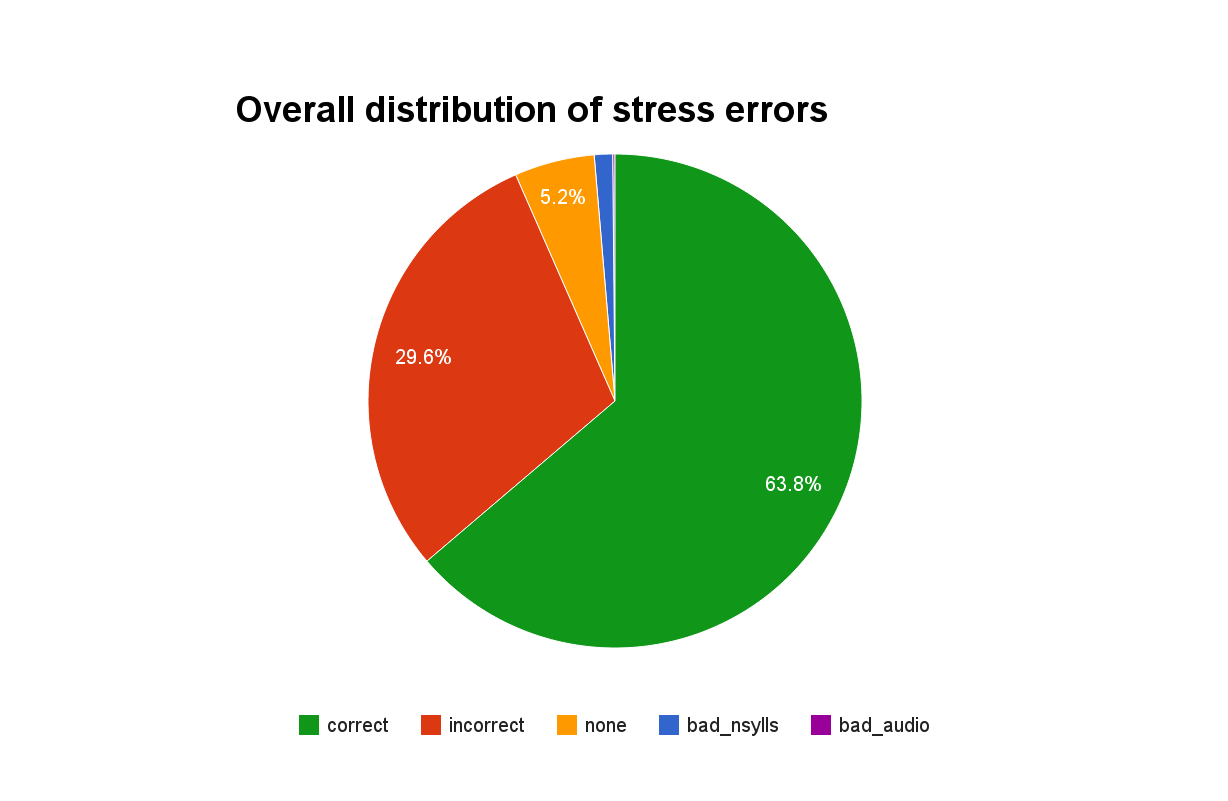
\includegraphics[width=\textwidth]{img/annotation/overallPie}
%			\caption{Overall distribution of lexical stress errors in the annotated corpus \TODO{retitle}}
%			\label{fig:results:overallpie}
%		\end{figure}
		
		\begin{figure}
			\centering
			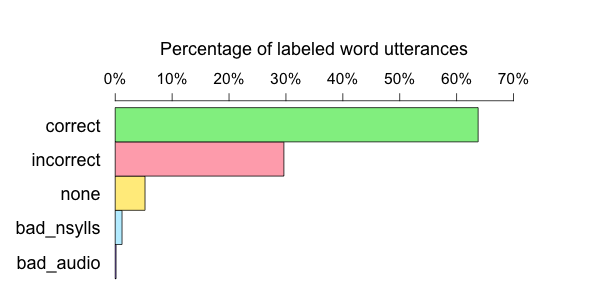
\includegraphics[width=.9\textwidth]{img/plots/overallJudgments-axisTop-noLabels}
			\label{fig:results:overallbars}
			\caption{Overall distribution of lexical stress errors in the annotated data}
		\end{figure}
		
		
		
		

		
		%\subsubsection{Accuracy by word type}
		\subsection{Errors by word type}
		\label{sec:results:wordtype}
		

\begin{table}[tbp]
				\centering
				\caption[Errors by word type]{Errors by word type: Number of tokens (utterances) assigned to each of the five categories, listed by word type. Equivalent percentages of each word type's total number of tokens are given in parentheses.}
				\begin{tabularx}{\textwidth}{lXXXXX}
				\toprule
				Word & correct & incorrect & none & bad\_nsylls & bad\_audio \\	
					\midrule
E-mail 			&	35 (62.5\%)	& 21 (37.5\%) 	&	0 					&	0 				&  0  				\\
Flagge			& 33 (60.0\%)	&	16 (29.1\%)	&	6 (10.9\%)	&	0 		 		&	0 					\\
fliegen 			&	46 (82.1\%)	&	7 (12.5\%) 	&	1 (1.8\%) 		&	2 (3.6\%)	&	0 					\\
Fr\"{u}hling 	&	48 (85.7\%) 	&	7 (12.5\%) 	&	1 (1.8\%)		&	0 				&	0 					\\
halten 			&	35 (62.5\%)	&	19 (33.9\%)	&	2 (3.6\%)		&	0				&	0 					\\
manche		&	36 (64.3\%)	&	17 (30.4\%)	&	1 (1.8\%)		&	1 (1.8\%) 	&	1 (1.79\%)	\\
M\"{o}rder	& 33 (58.9\%)	&	16 (28.6\%)	&	7 (12.5\%)	&	0 				&	0 					\\
Pollen			& 36 (64.3\%)	&	19 (33.9\%)	&	1 (1.8\%)		&	0 				&	0 					\\
Ringen			& 32 (58.2\%)	&	12 (21.8\%)	&	8 (14.6\%)	&	3 (5.5\%)	&	0 					\\
Tatort			& 20 (36.4\%)	&	32 (58.2\%)	&	2 (3.6\%)		&	1 (1.8\%)	&	0 					\\
tragen			& 32 (58.2\%)	&	23 (41.8\%)	&	0 					&	0 				&	0 					\\
Tschechen 	&	40 (71.4\%)	&	9 (16.1\%)	 &	6 (10.7\%)	&	1 (1.8\%) 	&	0  				\\
					\bottomrule
				\end{tabularx}
				\label{tab:results:wordtype}
			\end{table}		
		
			
			To take a more detailed look at the errors observed in the annotated data, error judgments were broken down by word type, with the results of this analysis presented in \cref{tab:results:wordtype} and illustrated in \cref{fig:results:wordbars}. 
			
			
			
%			\begin{table}[tbp]
%				\centering
%				\caption[Errors by word type]{Errors by word type \TODO{put \%s in parens and lose 2nd row} \TODO{omit 0 values?}}
%				\begin{tabularx}{\textwidth}{lrXrXrXrXrX}
%				\toprule
%				Word type & \multicolumn{2}{c}{correct}		& \multicolumn{2}{c}{incorrect} &		\multicolumn{2}{c}{none} &		\multicolumn{2}{c}{bad\_nsylls} & 		\multicolumn{2}{c}{bad\_audio} \\	
%				& $N$ & \% & $N$ & \% & $N$ & \% & $N$ & \% & $N$ & \% \\
%					\midrule
%E-mail &	35	& 62.50\%	&21&	37.50\%&	0	&0.00\%&	0	&0.00\%	& 0	& 0.00\% \\
%Flagge	& 33	&60.00\%	 &	16	 &	29.09\%	 &	6	 &	10.91\%	 &	0	 &	0.00\%	 &	0	 &	0.00\%\\
%fliegen &	46	&82.14\%	 &	7	 &	12.50\% &		1	 &	1.79\% &		2	 &	3.57\%	 &	0	 &	0.00\%\\
%Fr\"{u}hling &	48&	85.71\% &		7	 &	12.50\% &		1 &		1.79\%	 &	0	 &	0.00\% &		0	 &	0.00\%\\
%halten &	35	&62.50\%	 &	19	 &	33.93\%	 &	2 &		3.57\%	 &	0	 &	0.00\%	 &	0	 &	0.00\%\\
%manche&	36	&64.29\%	 &	17	 &	30.36\%	 &	1	 &	1.79\%	 &	1	 &	1.79\% &		1	 &	1.79\%\\
%M\"{o}rder	&33&	58.93\%	 &	16	 &	28.57\%	 &	7	 &	12.50\%	 &	0	 &	0.00\%	 &	0	 &	0.00\%\\
%Pollen	& 36	&64.29\%	 &	19	 &	33.93\%	 &	1	 &	1.79\%	 &	0	 &	0.00\%	 &	0	 &	0.00\%\\
%Ringen	& 32	&58.18\%	 &	12	 &	21.82\%	 &	8	 &	14.55\%	 &	3	 &	5.45\%	 &	0	 &	0.00\%\\
%Tatort	& 20	&36.36\%	 &	32	 &	58.18\%	 &	2	 &	3.64\%	 &	1	 &	1.82\%	 &	0	 &	0.00\%\\
%tragen	& 32	&58.18\%	 &	23	 &	41.82\%	 &	0	 &	0.00\%	 &	0	 &	0.00\%	 &	0	 &	0.00\%\\
%Tschechen &	40	&71.43\%&	9	 &	16.07\%	 &	6	 &	10.71\%	 &	1	 &	1.79\% &		0	 &	0.00\% \\
%					\bottomrule
%				\end{tabularx}
%				\label{fig:results:wordtype}
%			\end{table}
			
			
			
%			\begin{figure}[htb]
%				\centering
%				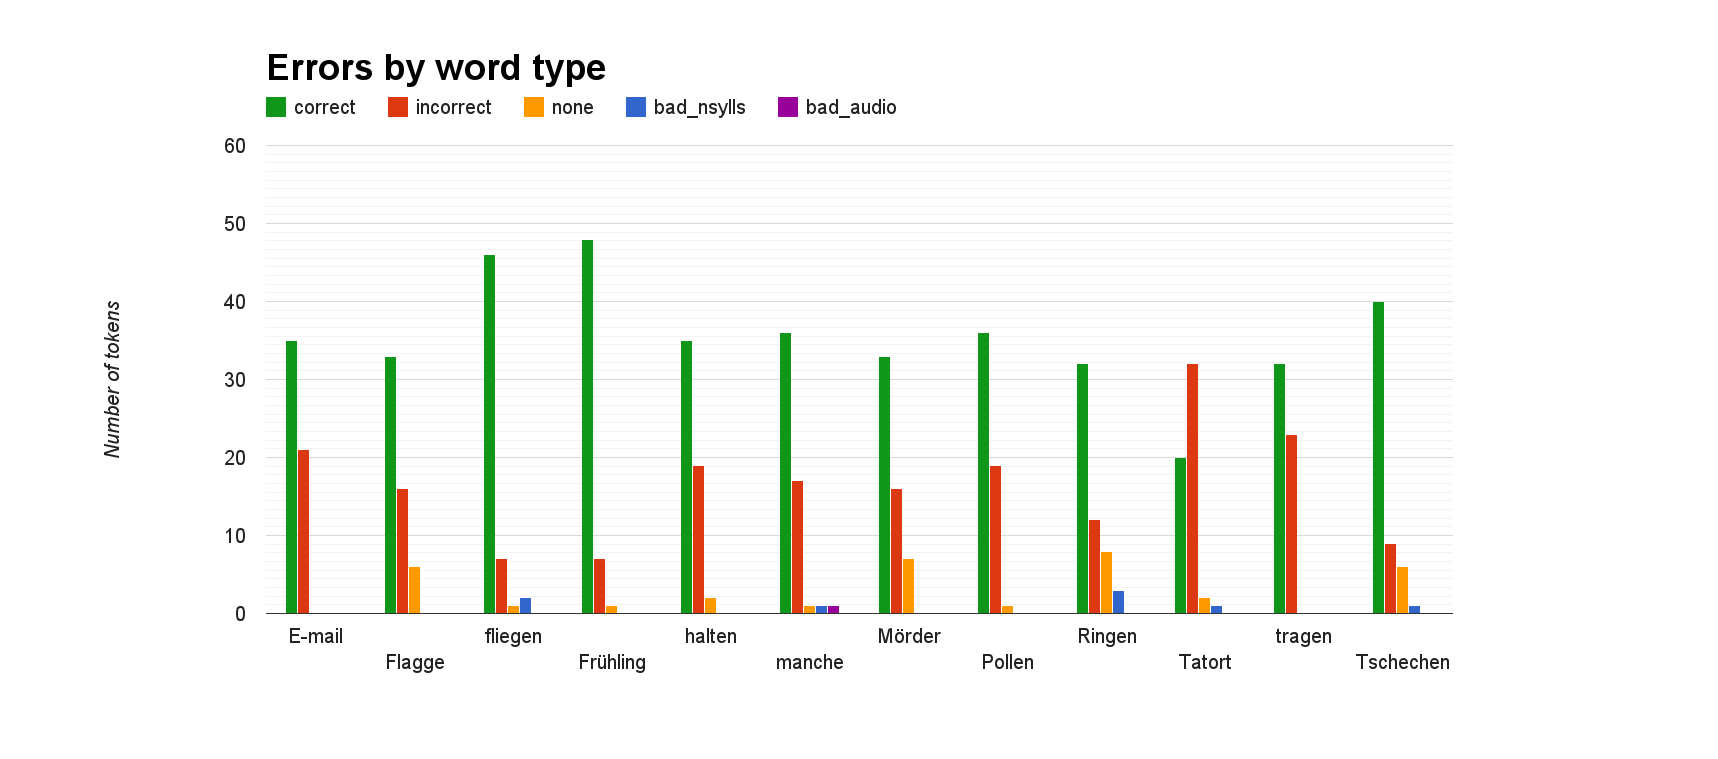
\includegraphics[width=\textwidth]{img/annotation/wordBars}
%				\caption{Errors by word type}
%				\label{fig:results:wordbars}
%			\end{figure}		

			\begin{figure}[tbp]
				\centering
				\caption[Error distribution by word type]{Distribution of errors by word type,
				as a percentage of the total number of labeled tokens (utterances) of that word type 
				(see \cref{tab:results:wordtypes} for precise values)
				}
				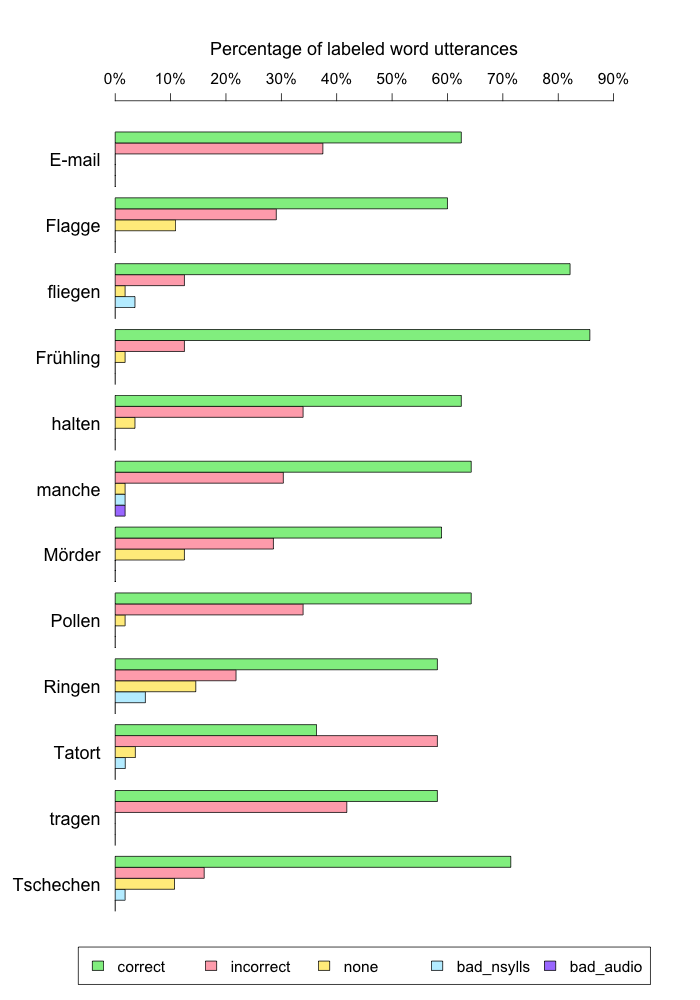
\includegraphics[width=\textwidth]{img/plots/judgmentsWordTypes}
				\label{fig:results:wordbars}
			\end{figure}	
			
			As should be expected, most word types exhibit a distribution of errors quite similar to the overall distribution, i.e. a ratio of correct to incorrect utterances of approximately 2:1, broadly speaking. However, for the words \textit{fliegen}, \textit{Fr\"{u}hling}, and \textit{Tschechen}, a much higher proportion of correct stress realizations was observed,
			%For the word \textit{tragen}, the number of incorrect realizations (23, or 41.82\%)was much closer to that of correct ones  (32, or 58.18\%) , 
			and for one word, \textit{Tatort}, incorrect realizations actually exceeded correct productions by a noticeable margin (32 or 58.18\% versus 20 or 36.36\%, respectively). 
			
			Unfortunately, no clear explanations for these discrepancies between word types readily present themselves, though a few speculations will be offered here. Of the words with uncommonly high proportions of correct utterances, two of the three (\textit{fliegen} and \textit{Fr\"{u}hling}) occurred in the same sentence in the IFCASL corpus --  \textit{In Fr\"uhling fliegen Pollen durch die Luft} -- along with another of the annotated word types, \textit{Pollen}. This sentence, in part due to the occurrence of these three bisyllabic initial-stress words in immediate succession, exhibits a very regular metrical pattern. With ``x'' and ``-'' indicating stressed and unstressed syllables, respectively, the sentence's rhythm can be represented as:
			%TODO {is this iambic or trochaic? explanation? reference?}:
			\begin{center}
			\begin{tabular}{llllllllll}
			In & Fr\"uh-& ling & flie-& gen & Pol-& len & durch & die & Luft \\
			- & x & - &  x & - & x & - & x & - & x \\
			\end{tabular}
			\end{center}
			As a result of this regularity, correctly realizing the prosody of each word in this sentence may present less of a challenge to L1 French speakers than a less regular sentence, and may thus explain their uncharacteristically flawless productions of the words therein. The fact that no fewer than the expected proportion of errors were observed in utterance of \textit{Pollen} would seem to contradict this speculative explanation; however, unlike the other words, \textit{Pollen} is doubly challenging for L1 French speakers, insofar as its first vowel is a short \textipa{O}, as opposed to the long \textipa{o:} in the word \textit{Polen} (meaning \textit{Poland} or \textit{Poles} in English), with which \textit{Pollen} forms a minimal pair.\footnote{This minimal pair was of interest to the researchers who constructed the IFCASL corpus, and \textit{Polen} also appears in the corpus, though it was not selected for inclusion in the dataset to be annotated for lexical stress errors.}  Differentiating between long and short vowels when speaking German may be another pronunciation challenge for French speakers \TODO{\citep{Zimmerer2015}}, as vowel length does not serve a contrastive function in French \citep{Peperkamp2002}. It may be the case that the short vowel in \textit{Pollen}, and the existence of another similar-sounding word, is responsible for some of the errors observed in the data, even though \textit{Pollen} and \textit{Polen} share the same stress pattern (stress on the initial syllable), for one of two reasons: either the added challenge of producing a difficult vowel in \textit{Pollen} distracts French speakers from the simple, regular prosody of the sentence, causing them to produce more prosodic errors with this word, or the native German annotators (most of whom, as discussed in \cref{sec:lexstress:annotators}, are not trained in phonetics or phonology) who are tasked with assessing the correctness of the word's prosody are distracted by the incorrect vowel quantity/quality in French speakers' productions of this word, and erroneously interpret the flaw(s) that they detect in the word's pronunciation as having to do with lexical stress, when in fact they are segmental errors. 
			It also seems plausible that frequency effects could be at play (\textit{Pollen} being ostensibly less frequent than \textit{Frühling} or \textit{fliegen}), or that there may be an influence from the word's position in the phrase/sentence (or interpreted position, in the case of L2 speakers inferring incorrect phrase boundaries).
			%\TODO{...or it could be word frequency (Pollen less frequent), or maybe influence of phrase position or interpreted phrase position, cf. \citep{Michaux2013}?}
			
			As for the uncharacteristically large proportion of errors in \textit{Tatort} (\textit{crime scene}), it may be the case that learners have difficulty identifying the boundary between syllables/morphemes in this word, which is a compound of the words \textit{Tat} (\textit{act}) and \textit{Ort} (\textit{place}).
			As \textit{Tatort} is quite possibly an unfamilar word to the learners, especially those with lower German proficiency, perhaps 
			this word's resemblance to the common French words \textit{ta} (\textit{your}) and \textit{tort} (\textit{wrong}) interferes with French speakers' production, such that they realize the word as the plausible French word sequence \textit{ta tort} (\textit{your wrong(doing)} or \textit{your mistake}), in which \textit{tort} would be more prominent.  
			%, its actual meaning in German being \textit{crime scene}.
			However, once again it should be noted that this
			% explanation is purely speculative
			%and 
			purely speculative explanation is not (and cannot be) verified by the data collected here.  
			
			
			
		
		
		
		%\subsubsection{Accuracy by L2 skill level}
		\subsection{Errors by L2 proficiency level}
		\label{sec:results:level}
		
		
		
			
			As \cref{sec:lexstress:data} stated, the L1 French speakers whose recordings comprise the dataset span four levels of L2 German proficiency: A2 (elementary), B1 (intermediate), B2 (upper intermediate), and C1 (advanced). The rightmost column of \cref{tab:results:levels} gives the number and proportion of utterances from speakers of each level in the dataset, along with the number of utterances from speakers of each level that were assigned to each of the five possible stress-accuracy labels, and these figures are illustrated in \cref{fig:levelbars:4}. Because the total number of utterances by speakers of each of the two intermediate (B) levels in the corpus is lower than the number by speakers of the lowest (A2) and highest (C1) levels, the judgments have also been grouped into two broader categories for easier comparison: beginners (A2 and B1) and advanced speakers (B2 and C1). The breakdown of stress errors by these groups is given in the lower portion of \cref{tab:results:levels} and illustrated in \cref{fig:levelbars:groups}.
			
			
			
%			\begin{table}
%				\begin{tabularx}{\textwidth}{XrXrXrXrXrXr}		
%				\toprule
%				 & \multicolumn{2}{c}{correct}		& \multicolumn{2}{c}{incorrect} &		\multicolumn{2}{c}{none} &		\multicolumn{2}{c}{bad\_nsylls} & 		\multicolumn{2}{c}{bad\_audio} & Total (\%) \\
%				\midrule			
%A2	&	137	&	47.74\%	&	118	&	41.11\%	&	26	&	9.06\%	&	5	&	1.74\%	&	1	&	0.35\%	&	287	(42.96\%)	\\
%B1	&	68	&	56.67\%	&	49	&	40.83\%	&	3	&	2.50\%	&	0	&	0.00\%	&	0	&	0.00\%	&	120 (17.96\%)	\\
%B2	&	52	&	72.22\%	&	17	&	23.61\%	&	3	&	4.17\%	&	0	&	0.00\%	&	0	&	0.00\%	&	72	(10.78\%)	\\
%C1	&	169	&	89.42\%	&	14	&	7.41\%	&	3	&	1.59\%	&	3	&	1.59\%	&	0	&	0.00\%	&	189	(28.29\%)	\\
%				\bottomrule
%				\end{tabularx}
%			\end{table}		

%		\begin{table}
%			\caption{Errors by speaker skill level}
%				\begin{tabularx}{\textwidth}{XXXXXXX}		
%				\toprule
%				 & correct	& incorrect &	none &		bad\_nsylls & 		{bad\_audio} & %\multicolumn{2}{c}{Total (\% corpus)} 
%				 \\
%				\midrule			
%A2	&	137	(47.7\%)	&	118	(41.1\%)	&	26 (9.1\%)	&	5	(1.7\%)		&	1	(0.4\%)		&	287	(43.0\%)	\\
%B1		&	68	(56.7\%)	&	49 	(40.8\%)	&	3	(2.5\%)		&	0					&	0					&	120	(18.0\%)	\\
%B2		&	52	(72.2\%) &	17	(23.6\%)	&	3	(4.2\%)		&	0					&	0					&	72	(10.8\%)	\\
%C1	&	169	(89.4\%) &	14	(7.4\%)		&	3	(1.6\%)		&	3	(1.6\%)		&	0					&	189	(28.3\%)	\\
%				\midrule					
%Beginner (A2,B1)	&	205	(50.4\%)	&	167	(41.0\%)	&	29 (7.1\%)	&	5	(1.2\%)	&	1	(0.3\%)	&	407	(60.9\%)	\\
%Advanced (B2,C1)	&	221	(84.7\%)	&	31	(11.9\%)	&	6	(2.3\%)	&	3	(1.2\%)	&	0					&	261	(39.1\%)	\\
%				\bottomrule
%				\end{tabularx}
%				\label{tab:results:levels}
%			\end{table}		
			
		\begin{table}
			\caption[Errors by L2 proficiency level]{Errors by L2 proficiency level: Number of tokens (utterances) assigned to each of the five categories, listed by the L2 German proficiency level of the speaker. Equivalent percentages of the total number of tokens for each level/level group are given in parentheses.}
			\setlength{\tabcolsep}{0.5mm}
			
			\begin{subtable}{\textwidth}
				\caption{Individual levels}
				\begin{tabularx}{\textwidth}{lrXrXrXrX}
				\toprule
					&	A2 & %\multicolumn{2}{l}{A2}					
					&	B1 & %\multicolumn{2}{l}{B1}						
					&	B2 & %\multicolumn{2}{l}{B2}							
					&	C1 & %\multicolumn{2}{l}{C1}					
					\\
				\midrule
correct			&	137 	& (47.7\%)	&	68	& (56.7\%)	&	52	& (72.2\%)	&	169	& (89.4\%)	\\
incorrect		&	118 	& (41.1\%)	&	49	& (40.8\%)	&	17	& (23.6\%)	&	14	& (7.4\%)		\\
none				&	26 	& (9.1\%)		&	3		& (2.5\%)		&	3		& (4.2\%)		&	3		& (1.6\%)		\\
bad\_nyslls	&	5		& (1.7\%)		&	0		&					&	0		&					&	3		& (1.6\%)		\\
bad\_audio	&	1		& (0.4\%)		&	0		&					&	0		&					&	0		&					\\
Total (\% of dataset)	&	287 & (43.0\%)	&	120 & (18.0\%)	&	72 & (10.8\%)	&	189 & (28.3\%)	\\
				\bottomrule
				\end{tabularx}
				\label{tab:results:levels:4}
			\end{subtable}
			
			\vspace{1em}
			
			\begin{subtable}{\textwidth}
				\caption{Level groups}
				\begin{tabularx}{\textwidth}{XrXrX}
				\toprule
					&	\multicolumn{2}{l}{Beginner (A2+B1)}					
					&	\multicolumn{2}{l}{Advanced (B2+C1)}									
					\\
				\midrule
correct			&	205	&	(50.37\%)	& 221	&	(84.67\%)	\\
incorrect		&	167	&	(41.03\%) & 31		&	(11.88\%)\\
none				&	29	&	(7.13\%)	& 6		&	(2.30\%)\\
bad\_nyslls	&	5		&	(1.23\%)	& 3		&	(1.15\%)\\
bad\_audio	&	1		&	(0.25\%) 	& 0		& 	\\
Total (\% of dataset)	&	407	&	(60.93\%) & 261	&	(39.07\%)	\\
				\bottomrule
				\end{tabularx}
				\label{tab:results:levels:groups}
			\end{subtable}
			
			\label{tab:results:levels}
		\end{table}
					
			
			\begin{figure}[tbp]
				\centering
				
				\begin{subfigure}{\textwidth}
					\centering
					\caption{Each level}
					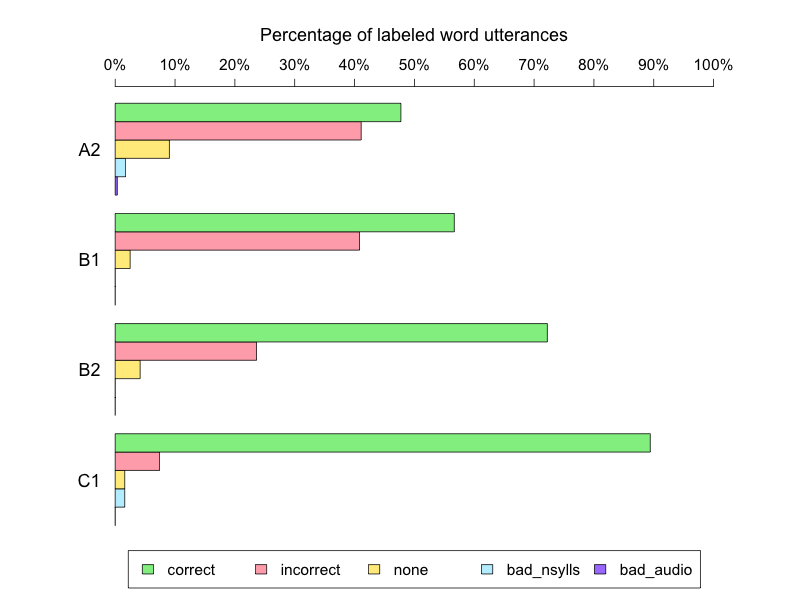
\includegraphics[width=\textwidth]{img/plots/judgments4Levels}
					\label{fig:levelbars:4}
				\end{subfigure}

				\vspace{1em}				
				
				\begin{subfigure}{\textwidth}
					\centering
					\caption{Level groups (Beginner is A2 + B1, Advanced is B2 + C1)}
					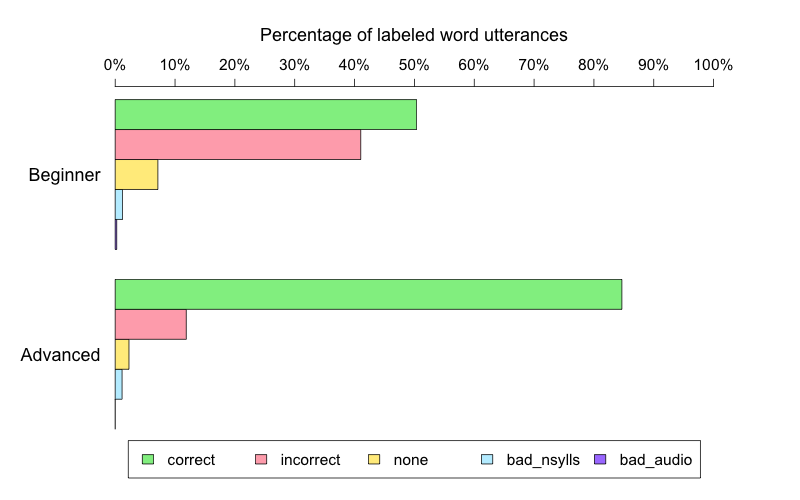
\includegraphics[width=\textwidth]{img/plots/judgmentsLevelGroups}
					\label{fig:levelbars:groups}
				\end{subfigure}
				
				
				%\caption{Stress judgments by speaker skill level}
				\caption[Error distribution by proficiency level]{Distribution of errors by speaker's L2 German proficiency level,
				as a percentage of the total number of labeled tokens (utterances) from speakers of that level/group 
				(see \cref{tab:results:levels} for precise values)
				}
				\label{fig:levelbars}
			\end{figure}
			
%			
%			\begin{figure}[ht]
%				\centering
%				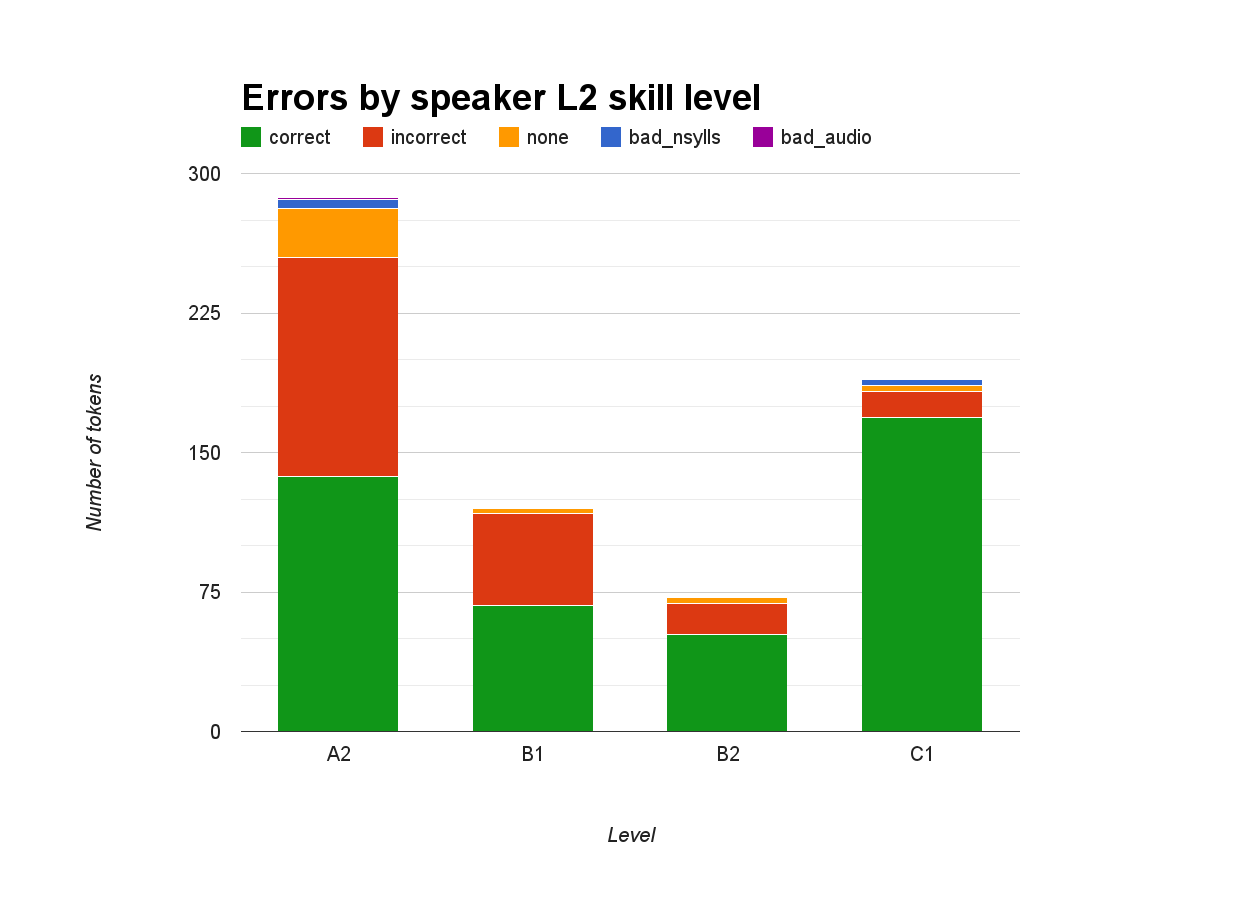
\includegraphics[width=\textwidth]{img/annotation/skillLevelBars}
%				\caption{Stress judgments by speaker skill level \TODO{Exclude?}}
%				\label{fig:levelbars}
%			\end{figure}
		
		
%			\begin{figure}[htb]
%				\centering
%				\begin{subfigure}[t]{0.5\textwidth}
%					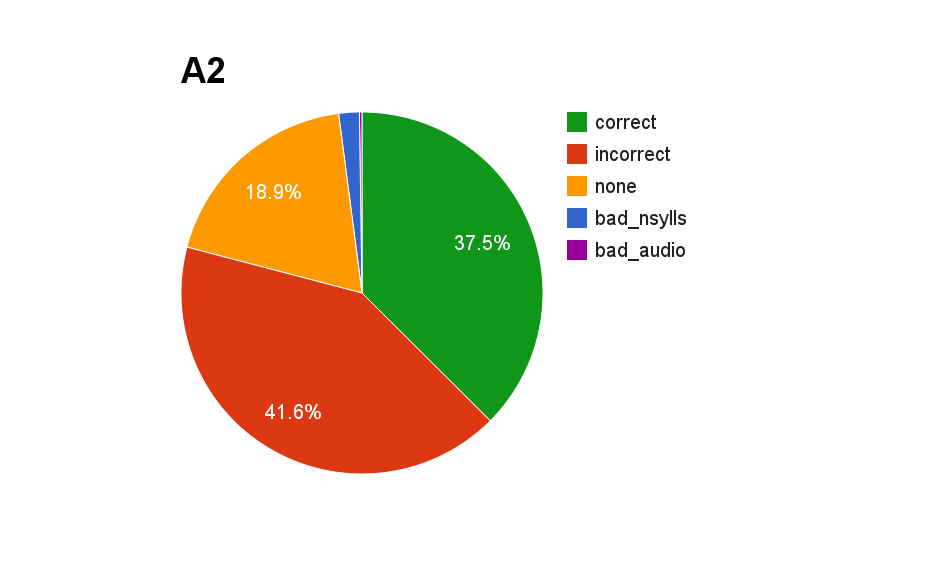
\includegraphics[width=\textwidth]{img/annotation/A2}
%					\caption{A2}
%					\label{fig:levelpies:A2}
%				\end{subfigure}%
%				~
%				\begin{subfigure}[t]{0.5\textwidth}
%					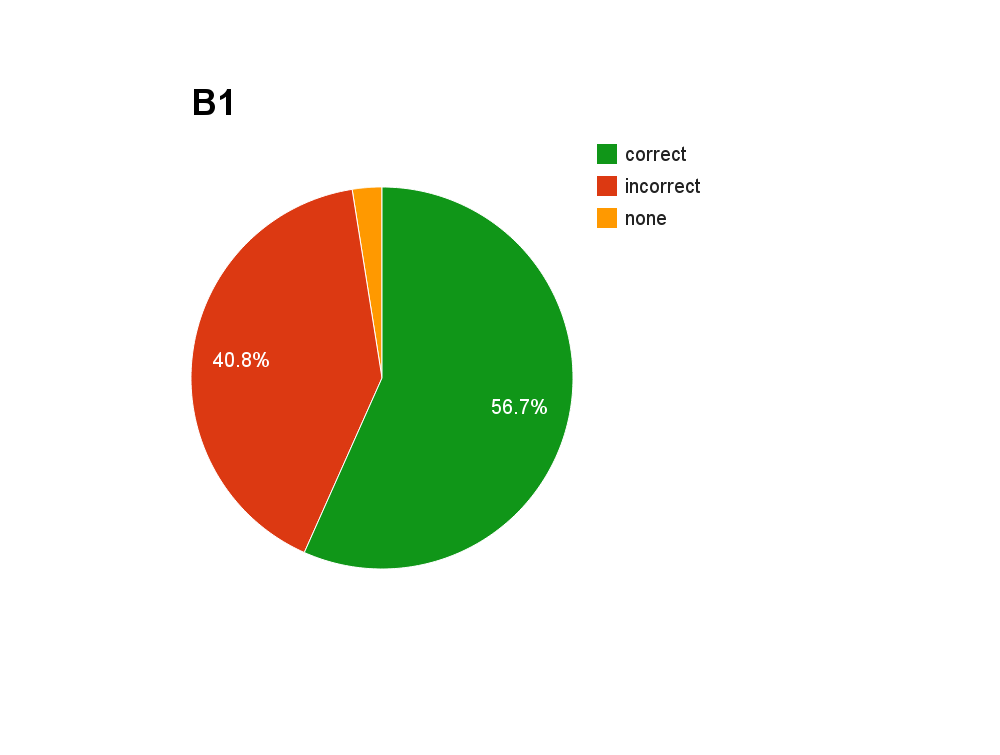
\includegraphics[width=\textwidth]{img/annotation/B1}
%					\caption{B1}
%					\label{fig:levelpies:B1}
%				\end{subfigure}%
%				
%				\begin{subfigure}[b]{0.5\textwidth}
%					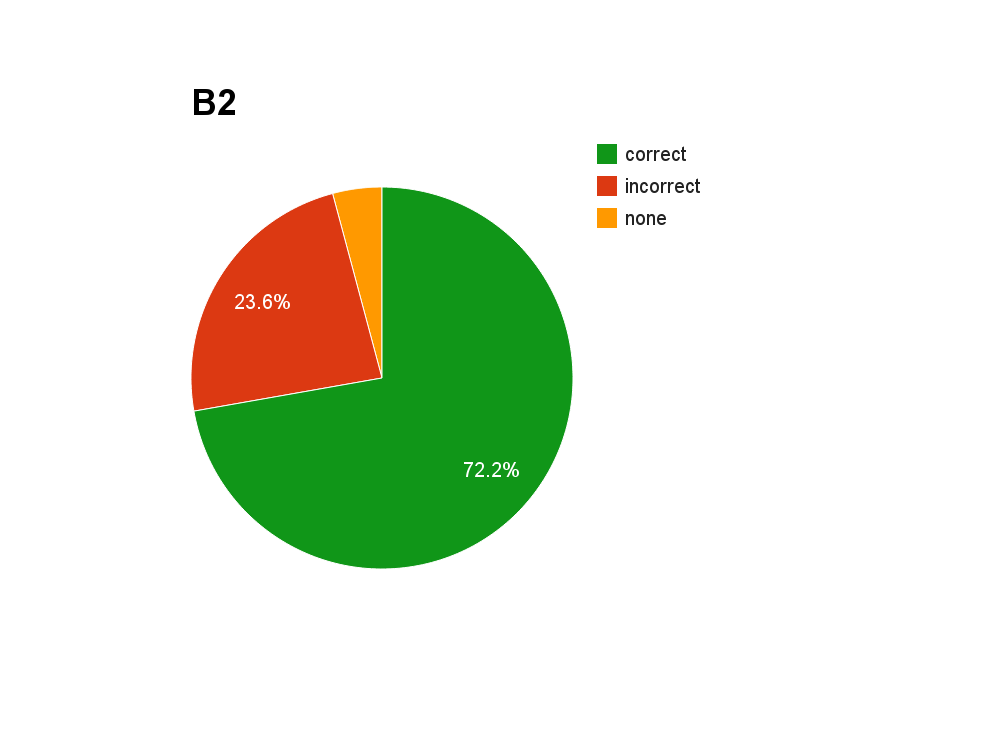
\includegraphics[width=\textwidth]{img/annotation/B2}
%					\caption{B2}
%					\label{fig:levelpies:B2}
%				\end{subfigure}%
%				~
%				\begin{subfigure}[b]{0.5\textwidth}
%					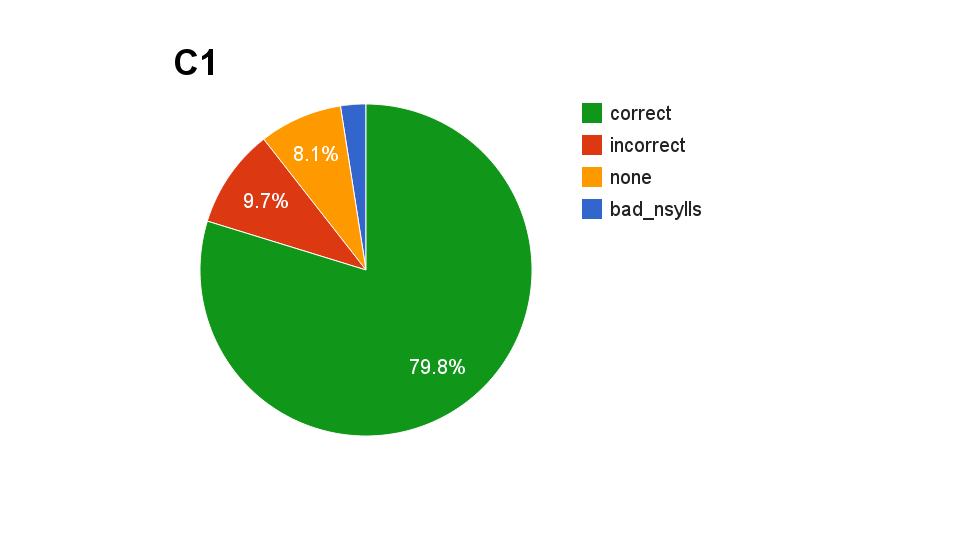
\includegraphics[width=\textwidth]{img/annotation/C1}
%					\caption{C1}
%					\label{fig:levelpies:C1}
%				\end{subfigure}%
%				\caption{Error distribution by speaker skill level}
%				\label{fig:levelpies}
%			\end{figure}		
			
			
			
			
			
			
%			\begin{table}
%			\begin{tabularx}{\textwidth}{lrXrXrXrXrXrX}		
%			\toprule
%			Group & \multicolumn{2}{c}{correct}		& \multicolumn{2}{c}{incorrect} &		\multicolumn{2}{c}{none} &		\multicolumn{2}{c}{bad\_nsylls} & 		\multicolumn{2}{c}{bad\_audio} & Total & \% of corpus \\
%			\midrule			
%				
%			\bottomrule
%			\end{tabularx}
%			\end{table}		
			
%			\begin{figure}[htb]
%				\centering
%				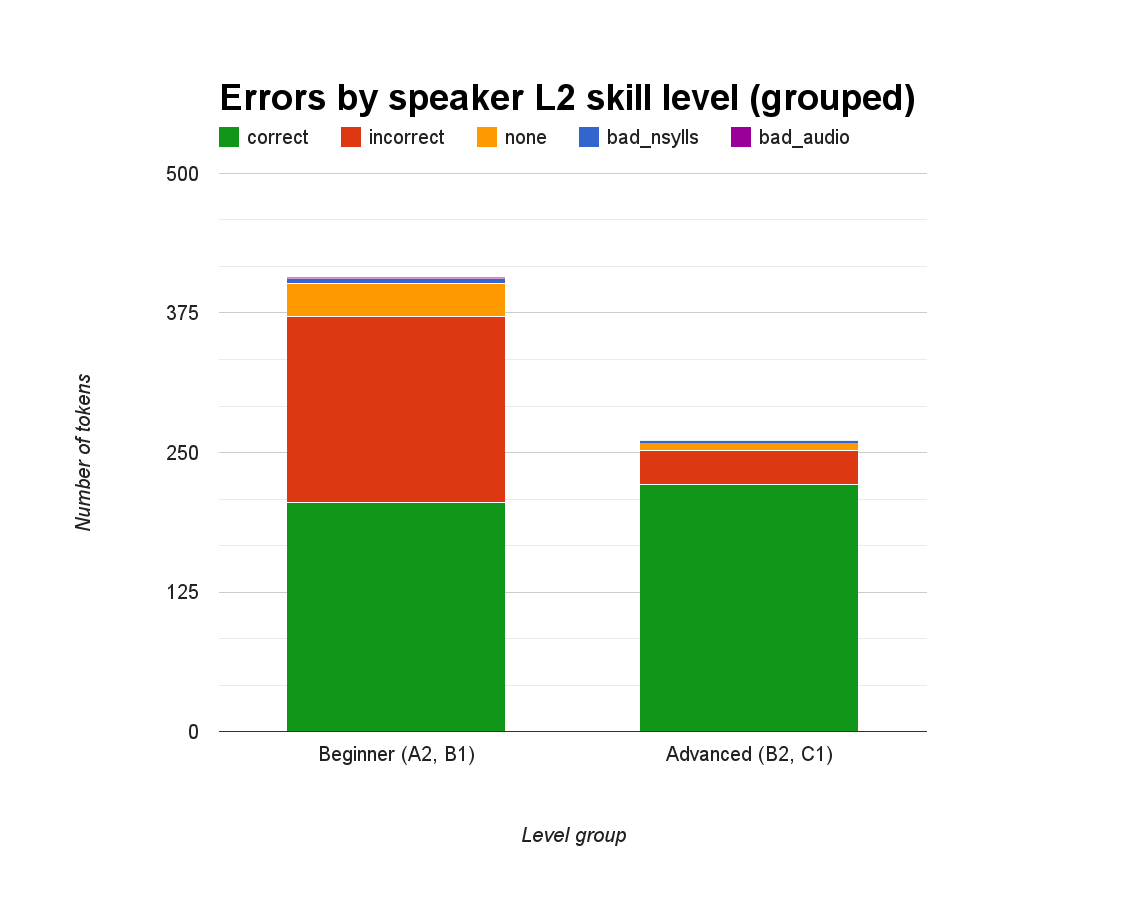
\includegraphics[width=\textwidth]{img/annotation/skillLevelGroupsBars}
%				\caption{Stress judgments by speaker skill level (grouped)}
%				\label{fig:levelgroupsbars}
%			\end{figure}
%			
%			
%			\begin{figure}[htb]
%				\centering
%				\begin{subfigure}[t]{0.5\textwidth}
%					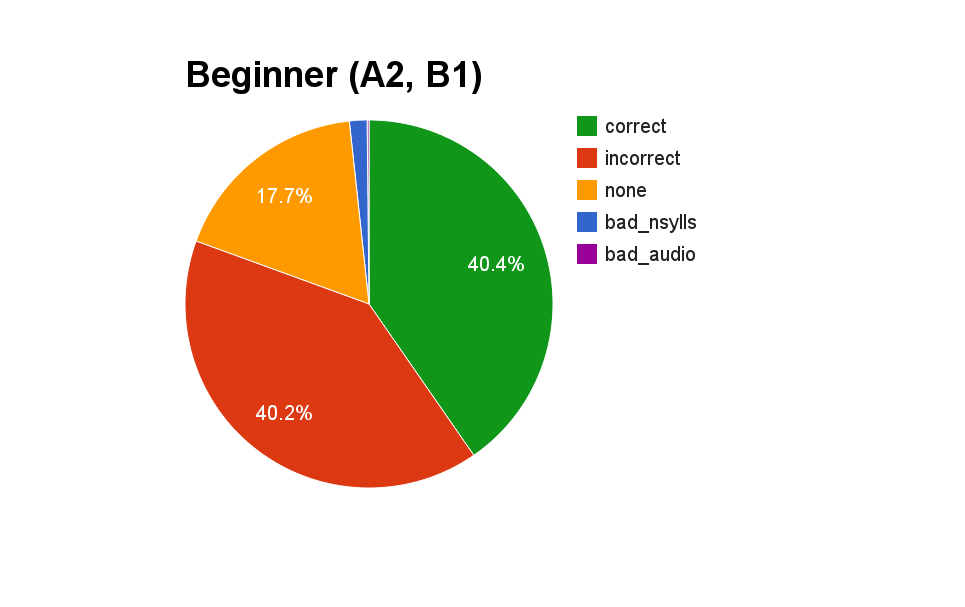
\includegraphics[width=\textwidth]{img/annotation/beginnerPie}
%					\caption{}
%					\label{fig:levelgroupspies:beg}
%				\end{subfigure}%
%				~
%				\begin{subfigure}[t]{0.5\textwidth}
%					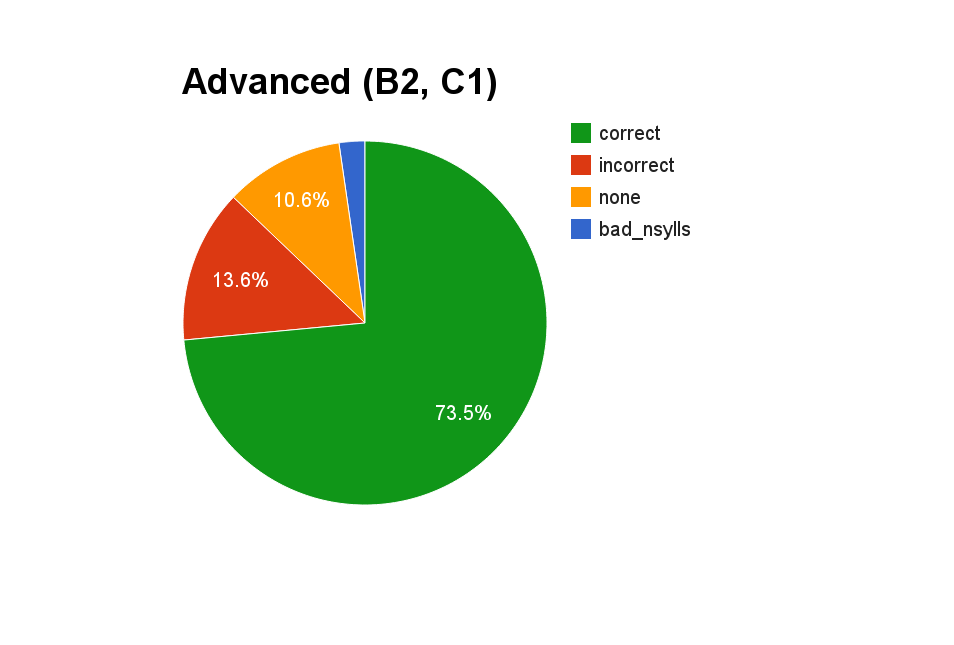
\includegraphics[width=\textwidth]{img/annotation/advancedPie}
%					\caption{}
%					\label{fig:levelgroupspies:adv}
%				\end{subfigure}%
%				\caption{Error distribution by speaker skill level (grouped)}
%				\label{fig:levelgroupspies}
%			\end{figure}	
			
			
	Unsurprisingly, these figures reveal that  speakers of the higher levels (B2 and C1) seem to make a proportionally lower number of errors than speakers of the lower ones (A2 and B1), with each level exhibiting a lower proportion of errors than the level below it. Generally speaking, beginners  (A2 and B1) seem to realize lexical stress correctly in about half of their utterances, whereas for upper intermediate (B2) learners the proportion of correct utterances is closer to three-fourths, and it approaches 90\% for advanced (C1) learners. As previously established (see \cref{sec:bkgd:targeting}), a CAPT system targeting a particular type of error will only be useful if that error is produced with considerable frequency by the learners using the system; therefore, it would seem from the frequency of lexical stress errors in their speech that learners of lower proficiency levels may benefit more from a CAPT system targeting such errors than learners of higher proficiency. 
			This conforms with findings of \textcite{Michaux2012}, which also seemed to indicate that, as might be expected, beginners make more lexical stress errors than advanced learners.
			
			
		
		\subsection{Errors by speaker age and gender}
		\label{sec:results:agegender}
			
			
			Given that the IFCASL corpus \citep{Fauth2014,Trouvain2013}, and by extension the dataset annotated for lexical stress errors, contains recordings from speakers of both genders and from adult speakers (18-30 years old) as well as children (adolescents ages 15-16) (see \cref{tab:data:speakers}), an analysis of the errors observed in terms of the age and gender of the speakers is of interest, to determine whether any discernible differences exist between the different groups of speakers. The breakdown of errors for each of these groups is presented in \cref{tab:results:agegender} and illustrated in \cref{fig:results:agegenderbars}.
			
			
			\begin{table}[p]
			\caption[Errors by speaker age and gender]{Errors by speaker age and gender: Number of tokens (utterances) assigned to each of the five categories, listed by the age/gender of the speaker. Equivalent percentages of the total number of tokens for each age/gender group are given in parentheses.}
			\setlength{\tabcolsep}{0.5mm}
			
			\vspace{1em}			
			
			\begin{subtable}{\textwidth}
				\centering
				\caption{Individual age/gender categories. Boys and Girls are males and females under the age of 18, respectively, and Men and Women are males and females over 18, respectively.}
				\begin{tabularx}{\textwidth}{lrXrXrXrX}
				\toprule
				& \multicolumn{2}{c}{Boys}% &
				& \multicolumn{2}{c}{Girls}% &
				& \multicolumn{2}{c}{Men}% &
				& \multicolumn{2}{c}{Women}% &
				\\
				\midrule
correct			&	48	&	(36.64\%)	&	6		&	(25.00\%)	&	184	&	(73.02\%)	&	188	&	(72.03\%)	\\
incorrect		&	60	&	(45.80\%)	&	17	&	(70.83\%)	&	61	&	(24.21\%)	&	60	&	(22.99\%)	\\
none				&	17	&	(12.98\%)	&	1		&	(4.17\%)	&	7		&	(2.78\%)	&	10	&	(3.83\%)	\\
bad\_nsylls	&	5		&	(3.82\%)	&	0		&					&	0		&					&	3		&	(1.15\%)	\\
bad\_audio	&	1		&	(0.76\%)	&	0		&					&	0		&					&	0		&		\\
Total (\%) of corpus)	&	131	&	(19.61\%)	&	24	&	(3.59\%)	&	252	&	(37.72\%)	&	261	&	(39.07\%)	\\
				\bottomrule
				\end{tabularx}
				\label{tab:agegender:4groups}
			\end{subtable}			
			
			\vspace{2em}
			
			\begin{subtable}{\textwidth}
				\centering
				\caption{By age, regardless of gender. Children are adolescents under age 18, adults are over 18. Adult beginners are adults with a German proficiency level of A2 or B1.}
				\begin{tabularx}{\textwidth}{lrXrXrX}
				\toprule
				& \multicolumn{2}{l}{Children}
				& \multicolumn{2}{l}{Adults}
				& \multicolumn{2}{l}{Adult beginners}
				\\
				\midrule
correct			&	54	&	(34.84\%)	&	372	&	(72.51\%)	&	151	&	(59.92\%)	\\
incorrect		&	77	&	(49.68\%)	&	121	&	(23.59\%)	&	90	&	(35.71\%)	\\
none				&	18	&	(11.61\%)	&	17	&	(3.31\%)	&	11	&	(4.37\%)	\\
bad\_nsylls	&	5		&	(3.23\%)	&	3		&	(0.58\%)	&	0		&		\\
bad\_audio	&	1		&	(0.65\%)	&	0		&					&	0		&		\\
Total (\%) of corpus)	&	155	&	(23.20\%)	&	513	&	(76.80\%)	&	252	&	(37.72\%)	\\
				\bottomrule
				\end{tabularx}
				\label{tab:agegender:age}
			\end{subtable}
			
			\vspace{2em}
			
			\begin{subtable}{\textwidth}
				%\centering
				\caption{By gender, regardless of age.}
				\begin{tabularx}{\textwidth}{XrXrX}
				\toprule
					&	\multicolumn{2}{l}{Males}					
					&	\multicolumn{2}{l}{Females}									
					\\
				\midrule
correct			&	232	&	(60.57\%)	&	194	&	(68.07\%)	\\
incorrect		&	121	&	(31.59\%)	&	77	&	(27.02\%)	\\
none				&	24	&	(6.27\%)	&	11	&	(3.86\%)	\\
bad\_nsylls	&	5		&	(1.31\%)	&	3		&	(1.05\%)	\\
bad\_audio	&	1		&	(0.26\%)	&	0		&		\\
Total (\% of corpus)	&	383	&	(57.34\%)	&	285	&	(42.66\%)	\\
				\bottomrule
				\end{tabularx}
				\label{tab:agegender:gender}
			\end{subtable}
			
			\label{tab:results:agegender}
			\end{table}
			
			
			\begin{figure}[ptb]
				\centering
								
				\begin{subfigure}{\textwidth}
					\centering
					\caption{Individual age/gender groups}
					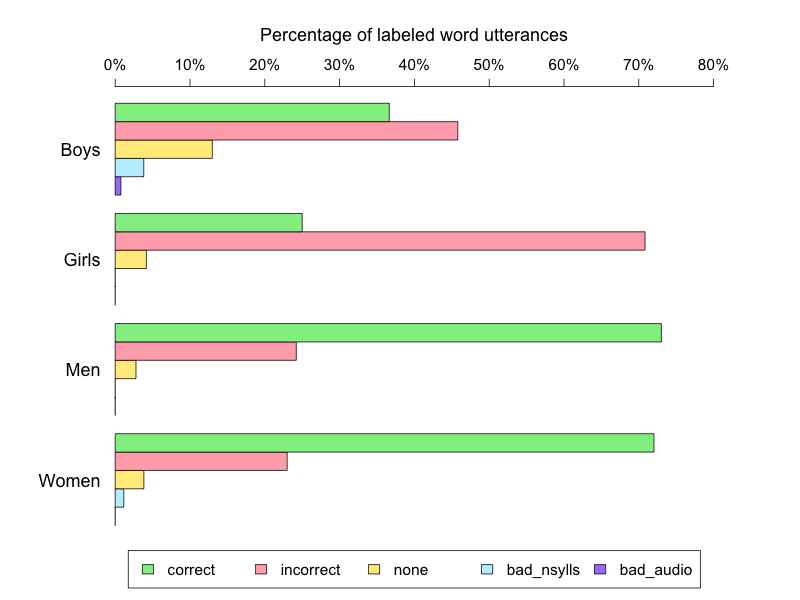
\includegraphics[width=\textwidth]{img/plots/judgmentsAgeGender}
					\label{fig:agegenderbars:4groups}
				\end{subfigure}
				
				\vspace{1.5em}
				
				\caption[Error distribution by speaker age and gender]{Distribution of errors by speaker's age and gender,
				as a percentage of the total number of labeled tokens (utterances) from speakers of that age/gender group
				(see \cref{tab:results:agegender} for precise values)
				}
				\ContinuedFloat
				
				\label{fig:results:agegenderbars}
			\end{figure}
			
			\begin{figure}[p]
			\ContinuedFloat
			\centering
			
				\begin{subfigure}{\textwidth}
					\setcounter{subfigure}{1}
					\centering
					\caption{By age, regardless of gender}
					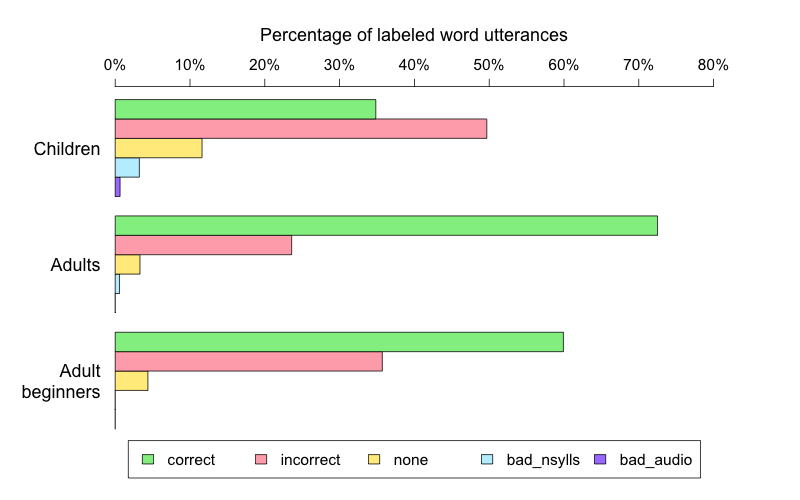
\includegraphics[width=\textwidth]{img/plots/judgmentsAge}
					\label{fig:agegenderbars:age}
				\end{subfigure}
				
				\vspace{1em}
			
				\begin{subfigure}{\textwidth}
					\centering
					\caption{By gender, regardless of age}
					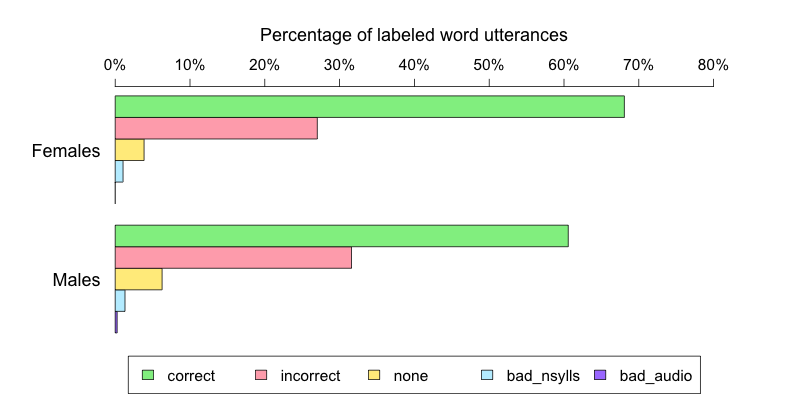
\includegraphics[width=\textwidth]{img/plots/judgmentsGender}
					\label{fig:agegenderbars:gender}
				\end{subfigure}
				
				\vspace{1.5em}
				
				\caption[Error distribution by speaker age and gender (cont.)]{(continued) Distribution of errors by speaker's age and gender,
				as a percentage of the total number of labeled tokens (utterances) from speakers of that age/gender group
				(see \cref{tab:results:agegender} for precise values)
				}
				
			\end{figure}
					
			
			
			

				With regard to the two different age groups of speakers, any interpretation of the results presented here must bear in mind the considerable difference in size between the groups (43 adults vs. 13 children): of the 668 tokens annotated in total, 513 (over three-fourths) were from adult speakers while only 155 (less than one-fourth) were utterances by children. Furthermore, it must be highlighted that there is a strong interaction between age and proficiency level: as seen in \cref{tab:data:speakers}, all of the child speakers 
				represented in the data 
				%recorded in the IFCASL corpus 
				are beginners 
				(the majority at the A2 level with only 1 girl at B1),
				% \TODO{technically true but implies A2 while a couple of the girls are B1 - worth mentioning?}, 
				while the adults span all four levels. Given the discrepancies between L2 proficiency levels discussed in the previous section, then, it is not surprising to see that over half of children's utterances are judged to have lexical stress errors, with correct stress productions making up only 35.1\% of utterances (54 utterances) by this age group. Adults, on the other hand, seem to realize lexical stress correctly in the majority of their utterances, with only 23.6\% (121) incorrect productions and 3.3\% percent (17) utterances with no clear lexical stress realization ([none]). However, this is not an entirely just comparison, given that the group of child speakers only includes beginners; instead of comparing the children's error distribution to that of all adults, it may be helpful to restrict the comparison to adults of the lower proficiency levels. 
				%The bottom rows of \cref{tab:results:agegender} list
				%\Cref{tab:results:agegender} lists the statistics for 
				%\TODO{\textit{remove?:} adults at the A2 proficiency level only as well as for}
				%adults of both beginner levels (A2 and B1), 
				%and \cref{fig:results:agepies:adultbeg} illustrates the error distribution for the latter group \TODO{include adult A2 chart also/instead? (distribution is quite similar to A2/B1)}. 
				Therefore, in addition to the results for all adults, \cref{tab:agegender:age} and \cref{fig:agegenderbars:age} display results for the group of adult beginners (level A2 or B1).
				
				Comparing the distribution of children's errors to that of adult beginners, the difference is less drastic but still noticeable, as adult beginners realize lexical stress correctly in the majority (approximately 60\%) of their utterances. Considering the comparatively high proportion of lexical stress errors in children's speech, therefore, it seems that 
				just as the results reported in the previous section seem to indicate that beginners may benefit more from a lexical stress CAPT system than advanced learners, 
				it may also be the case that
				children in particular stand to gain more from such a system than adult beginners.
%				in the same way that the results reported in the sa
%				just as \TODO{we} concluded in the previous section 
%				that beginners may benefit more from a CAPT system targeting lexical stress errors than advanced learners would, 
%				so also may children stand to gain more from such a system than adult beginners. 
%				
				
					Coming now to the question of whether there is any difference in error distribution between speakers of different genders, a brief glance at \cref{tab:agegender:gender,fig:agegenderbars:gender} reveals that there does not seem to be a drastic difference in the distribution of errors between the two genders. Males seem to make slightly more errors in lexical stress realization than females, with 60.7\% correct productions for males and 68.1\% for women, though this might be explained by the fact that as noted in \cref{sec:lexstress:data} above (see \cref{tab:data:speakers}), the group of male speakers has a higher proportion of elementary (A2) learners (18 out of 32 males, or 56.25\%) than the group of female speakers (6 A2 speakers out of 24 females, or 25\%). Therefore, it would seem that the error distribution observed in the annotated dataset provides no indication of a meaningful difference in the way speakers of different genders realize lexical stress in their L2 German.
				
					
			
			
			
%			\begin{figure}[ptb]
%				\centering
%				\caption[Error distribution by speaker age and gender]{Distribution of errors by speaker's age and gender,
%				as a percentage of the total number of labeled tokens (utterances) from speakers of that age/gender group
%				(see \cref{tab:results:agegender} for precise values)
%				}
%				\ContinuedFloat
%				
%				\vspace{1em}
%				
%				\begin{subfigure}{\textwidth}
%					\centering
%					\caption{Individual age/gender groups}
%					\includegraphics[width=\textwidth]{img/plots/judgmentsAgeGender}
%				\end{subfigure}
%				
%			\end{figure}
%			
%			\begin{figure}[p]
%			\ContinuedFloat
%			\centering
%				\caption[Error distribution by speaker age and gender (cont.)]{(continued) Distribution of errors by speaker's age and gender,
%				as a percentage of the total number of labeled tokens (utterances) from speakers of that age/gender group
%				(see \cref{tab:results:agegender} for precise values)
%				}
%				
%				\vspace{1em}
%				
%				\begin{subfigure}{\textwidth}
%					\setcounter{subfigure}{1}
%					\centering
%					\caption{By age, regardless of gender}
%					\includegraphics[width=\textwidth]{img/plots/judgmentsAge}
%				\end{subfigure}
%				
%				\vspace{1em}
%			
%				\begin{subfigure}{\textwidth}
%					\centering
%					\caption{By gender, regardless of age}
%					\includegraphics[width=\textwidth]{img/plots/judgmentsGender}
%				\end{subfigure}
%				
%				
%				
%				\label{fig:results:agegenderbars}
%			\end{figure}
%		
			
%			\begin{table}[h]
%				\caption[Errors by speaker age and gender]{Errors by speaker age and gender \TODO{add \%ages}}
%				\begin{tabularx}{\textwidth}{XXXXXXXX}			
%				\toprule
%Group	&	correct	&	incorrect	&	none	&	bad\_ nsylls	&	bad\_ audio	&	Total	&	\% of corpus	\\
%				\midrule
%Boys	&	48	&	60	&	17	&	5	&	1	&	131	&	19.61\%	\\
%Girls	&	6	&	17	&	1	&	0	&	0	&	24	&	3.59\%	\\
%Men	&	184	&	61	&	7	&	0	&	0	&	252	&	37.72\%	\\
%Women	&	188	&	60	&	10	&	3	&	0	&	261	&	39.07\%	\\
%
%\midrule		
%Children	&	54	&	77	&	18	&	5	&	1	&	155	&	23.20\%	\\													
%Adults	&	372	&	121	&	17	&	3	&	0	&	513	&	76.80\%	\\
%Adults (A2~only) & 86 & 49 & 9 & 0 & 0 & 144 & 21.56\%\\
%Adults (A2,~B1) &  151 & 90 & 11 & 0 & 0 & 252 & 37.72\%\\
%
%\midrule															
%Females	&	194	&	77	&	11	&	3	&	0	&	285	&	42.66\%	\\
%Males	&	232	&	121	&	24	&	5	&	1	&	383	&	57.34\%	\\
%				\bottomrule	
%				\end{tabularx}
%				\label{tab:results:agegender}
%			\end{table}
			
			
%			\begin{figure}[htb]
%				\centering
%				\includegraphics[width=\textwidth]{img/annotation/ageGenderBars}
%				\caption{Stress judgments by speaker age/gender}
%				\label{fig:results:agegenderbars}
%			\end{figure}
%			
			
%			\begin{figure}[htb]
%				\centering
%				\begin{subfigure}[t]{0.5\textwidth}
%					\includegraphics[width=\textwidth]{img/annotation/childPie}
%					\caption{Children}
%					\label{fig:results:agepies:child}
%				\end{subfigure}%
%				~
%%				\begin{subfigure}[t]{0.5\textwidth}
%%					\includegraphics[width=\textwidth]{img/annotation/adultPie}
%%					\caption{Adults \TODO{remove?}}
%%					\label{fig:results:agepies:adult}
%%				\end{subfigure}%
%%		
%				\begin{subfigure}[t]{0.5\textwidth}
%					\includegraphics[width=\textwidth]{img/annotation/adultBeginnersPie}
%					\caption{Adult beginners}
%					\label{fig:results:agepies:adultbeg}
%				\end{subfigure}%
%				
%				\caption{Error distribution by speaker age}
%				\label{fig:results:agepies}
%			\end{figure}	
%			
%			\begin{figure}[htb]
%				\centering
%				\begin{subfigure}[t]{0.5\textwidth}
%					\includegraphics[width=\textwidth]{img/annotation/femalePie}
%					\caption{Females}
%					\label{fig:results:genderpies:female}
%				\end{subfigure}%
%				~
%				\begin{subfigure}[t]{0.5\textwidth}
%					\includegraphics[width=\textwidth]{img/annotation/malePie}
%					\caption{Males}
%					\label{fig:results:genderpies:male}
%				\end{subfigure}%
%				\caption{Error distribution by speaker gender}
%				\label{fig:results:genderpies}
%			\end{figure}	
			
			
			
				
%				\begin{figure}[htb]
%				\centering
%				\begin{subfigure}[t]{0.5\textwidth}
%					\includegraphics[width=\textwidth]{img/annotation/adultA2Pie}
%					\caption{Adults of A2 skill level}
%					\label{fig:results:adultbeginners:a2}
%				\end{subfigure}%
%				~
%				\begin{subfigure}[t]{0.5\textwidth}
%					\includegraphics[width=\textwidth]{img/annotation/adultBeginnersPie}
%					\caption{Adult beginners (A2 and B1)}
%					\label{fig:results:adultbeginners:a2b1}
%				\end{subfigure}%
%				\caption{Error distribution for adult beginners}
%				\label{fig:results:adultbeginners}
%			\end{figure}	
				
				
		
%		\subsection{Errors by recording condition}
%		\label{sec:results:condition}
%			\TODO{}
%		
%		\begin{table}
%			\centering
%			\caption{Stress judgments by recording condition}
%			\begin{tabular}{lrrrr}
%			\toprule
%	Judgment	&	SH tokens	&	\% of SH	&	SR tokens	&	\% of SR	\\
%	\midrule
%	correct	&	97	&	58.79\%	&	329	&	65.41\%	\\
%	incorrect	&	51	&	30.91\%	&	147	&	29.22\%	\\
%	none	&	14	&	8.48\%	&	21	&	4.17\%	\\
%	bad\_nsylls	&	3	&	1.82\%	&	5	&	0.99\%	\\
%	bad\_audio	&	0	&	0.00\%	&	1	&	0.20\%	\\
%	\midrule
%	Total	&	165	&		&	503	&		\\
%	\% of corpus	&	24.70\%	&		&	75.30\%	&		\\	
%	\bottomrule
%			\end{tabular}
%			\label{tab:results:condition}
%		\end{table}
%		
%		\begin{figure}[htb]
%				\centering
%				\begin{subfigure}[t]{0.5\textwidth}
%					\includegraphics[width=\textwidth]{img/annotation/SRpie}
%					\caption{Sentence Read}
%					\label{fig:results:conditionpies:SR}
%				\end{subfigure}%
%				~
%				\begin{subfigure}[t]{0.5\textwidth}
%					\includegraphics[width=\textwidth]{img/annotation/SHpie}
%					\caption{Sentence Heard}
%					\label{fig:results:conditionpies:SH}
%				\end{subfigure}%
%				\caption{Error distribution by recording condition}
%				\label{fig:results:conditionpies}
%			\end{figure}			
%		
%	
%		\subsection{Impact of technical problems \TODO{remove?}}
%		\label{sec:results:techproblems}
%			\TODO{remove?}
	
	
	\section{Summary}
	\label{sec:lexstress:summary}

	In an effort to shed light on the nature of lexical stress errors in the speech of L1 French learners of German as L2, this chapter has described original efforts to 
	annotate such errors in a small corpus of learner speech, 
	%with this error-annotated data being used not only to 
	study the frequency and type of errors made by learners,
	%but also to 
	and analyze differences in how these errors are perceived by L1 and L2 German speakers with varying levels of phonetics/phonology expertise.
	
	As described in \cref{sec:lexstress:data,sec:lexstress:annotators,sec:lexstress:method},
	lexical stress realizations in utterances of bisyllabic, initial-stress words (\cref{sec:lexstress:data})
	%taken from the IFCASL corpus (\cite{Trouvain2013,Fauth2014}; see also \cref{sec:intro:ifcasl}) 
	were evaluated by multiple annotators from different L1 and phonetic training backgrounds (\cref{sec:lexstress:annotators}).
	Annotators were asked to use a graphical annotation tool to label each recorded word utterance
	as correctly or incorrectly realizing lexical stress (i.e. the speaker clearly stressed the correct or incorrect syllable), failing to clearly realize stress (i.e. the speaker did not seem to stress either syllable), or having technical or other problems which prevented the assessment of lexical stress (\cref{sec:lexstress:method}). 
	
	
	
	Analysis of the labels assigned by different annotators to the same utterances (\cref{sec:lexstress:agreement}) revealed that inter-annotator agreement was relatively low, with only ``fair'' agreement \citep{Landis1977}, on average, between each pair of annotators who labeled the same utterances. Considerable variation was observed among individual annotators (\cref{sec:agreement:overall}), which did not seem to be explained by differences among annotators in terms of their L1 (\cref{sec:agreement:native}) or level of experience with phonetics/phonology or speech data annotation (\cref{sec:agreement:expert}). 
	%\TODO{Stat significance?} 
	However, some other differences were observed in how different groups of annotators labeled lexical stress errors; specifically, L2 German speakers annotated a higher proportion of utterances as having unclear stress compared to L1 speakers (\cref{sec:agreement:native}), and expert annotators judged substantially higher proportion of utterances as correctly realizing stress compared to intermediate or novice annotators (\cref{sec:agreement:expert}).
	As described in \cref{sec:agreement:overall}, there also seemed to be variability in inter-annotator agreement with respect to the different word types represented in the dataset, though further work is needed to discern the factors responsible for this observation (see \cref{sec:conclusion:future}).
	
	The multiple, often conflicting, error annotations from different annotators were consolidated into a single gold-standard annotation for each utterance in the dataset (see \cref{sec:agreement:gold}), which served as the basis for an analysis of the frequency and type of errors produced by learners, as presented in \cref{sec:lexstress:results}. This analysis seemed to confirm the expectation set out in \cref{sec:stress:expected,sec:targeting:frequency} that lexical stress errors are quite frequent in the speech of French speakers of German, with correct lexical stress realizations observed in only approximately two-thirds of utterances, on average (\cref{sec:results:overall}). A finer-grained analysis revealed that the frequency of such errors appeared considerably lower in the speech of advanced learners than that of beginners (\cref{sec:results:level}), and that children seemed to make more errors than adult beginners (\cref{sec:results:agegender}); no substantial difference was observed between speakers of different genders. 
	%\TODO{stat significance?} 
	As in the case of inter-annotator agreement, considerable variation was observed in the frequency of errors in utterances of different word types (\cref{sec:results:wordtype}), though once again the factors underlying this variability are not immediately evident and should be investigated in future work (see \cref{sec:conclusion:future}).
	
	
	The error annotation and analysis described in this chapter thus contribute considerably to our understanding of the difficulties L1 French speakers may have realizing lexical stress in their L2 German speech, and the fact that learners, especially beginners and children, seem to struggle with lexical stress production justifies the selection of lexical stress errors as the focus of this thesis project. Additionally, the analysis of inter-annotator agreement presented in this chapter, specifically the finding that the observed agreement was generally rather low,
	constitutes an important discovery with respect to the task of identifying such errors in learner speech:
	%: namely, that this task may be challenging for certain L1 and L2 German speakers. 
	though further research is needed to determine why and under which conditions this is the case (see \cref{sec:conclusion:future}), it would seem that diagnosing lexical stress errors may be a challenging task for at least some L1 and L2 German speakers. If true, this has important implications for the development and evaluation of automatic error diagnosis systems, the subject of the following chapter, and these implications will be discussed further in \cref{sec:diag:classification}.
		% INCLUDE: lexical stress errors
\chapter{System overview}
\label{chap:system}		% INCLUDE: system overview
% DIAGNOSIS
%
% !TEX root = ../thesis-main.tex
%
\chapter{Diagnosis of lexical stress errors}
\label{chap:diagnosis}

%\cleanchapterquote{You can’t do better design with a computer, but you can speed up your work enormously.}{Wim Crouwel}{(Graphic designer and typographer)}

In order to provide learners with useful feedback on their lexical stress errors in the L2, 
the prototype CAPT tool developed in this thesis project 
must first be able to automatically detect and diagnose such errors in a learner's utterance. This requires at least:
\begin{enumerate}[label=(\alph*)]
\item Reasonably accurate word-, syllable- and phone-level segmentation of the learner's L2 utterance; 
\item %A means of analyzing
An analysis of how lexical stress is realized in the
% prosody of the segmented 
given
utterance;
\item A representation of how native speakers of the target language (would) realize lexical stress in the given sentence; and
\item %A way of comparing
A comparison of the learner's prosody to this representation. 
\end{enumerate}

This chapter describes 
%
how (a) is achieved using
 forced-alignment segmentation of a learner's read-speech utterance with the corresponding text, 
 %and how problems in accuracy of the resulting segmentation can be overcome 
 (\cref{sec:diag:segmentation}); 
 %
 how the lexical stress analysis of (b), which is also crucial to (c), is produced by measuring the fundamental frequency, duration, and energy of relevant sections of the speech signal (\cref{sec:diag:prosody}); 
 %
 and 
 %finally, 
 the various approaches to (c) and (d) that are implemented in the prototype tool (\cref{sec:diag:compare,sec:diag:classification}).
 Finally, it describes how the system's modular architecture allows researchers and teachers control over which of these approaches are used \TODO{(\cref{sec:diag:system})}.



\section{Automatic segmentation of nonnative speech}
\label{sec:diag:segmentation}

\TODO{Should this become a subsection of \cref{sec:diag:prosody}?}

%Automatic 
Segmentation, or labeling, of a recorded utterance is the task of annotating the speech signal with boundaries that demarcate individual phones, syllables, words, sentences, and/or other units of speech; see \cref{fig:GGsegmentation} for an example of a multi-level segmentation of a German utterance. 
	
	\begin{figure}
		\centering
		\includegraphics[width=\textwidth]{img/screenshots/SampleGG-basic}
		\caption[An example German utterance and its segmentation]{\TODO{update with new example w/ SyllableTier} An example of a German utterance that has been segmented at the phone level (first row) and word level (second row). The third row contains the canonical (expected) native pronunciation of each word in the sentence, while the fourth row contains the written sentence of which the utterance is a reading.}
		\label{fig:GGsegmentation}
	\end{figure}


A reasonably accurate segmentation of an L2 learner's utterance is indispensable for an analysis of the accuracy of their pronunciation; 
\TODO{mention that there are methods which don't need segmentation, but they're more limited?}
as it allows comparison between relevant units of the learner's utterance -- e.g. words, syllables, and phones -- and corresponding units in native speech. 
The most accurate segmentation would of course be one produced by hand by a trained phonetician. However, hand-labeling is not feasible in most scenarios because of its high cost in terms of time and wages; moreover, because the ultimate goal of this work is the development of a CAPT tool which can give L2 learners helpful automatic feedback on their pronunciation, 
%even when they do not have access to a language teacher, 
any analysis of the learner's speech signal, including the preliminary step of segmentation, must proceed fully automatically. Therefore, a means of automatically segmenting a given utterance is required.



	%\subsection{Segmentation via forced alignment}
	%\label{sec:segmentation:alignment}
	
	When the content (text) of a given utterance is already known, the goal of automatic segmentation becomes aligning the  boundaries of each phone in the expected sentence with the appropriate points in the recorded signal. Boundaries for larger units such as syllables and words can be inferred from the phone boundaries. 
	An effective and widely-used technique for this is 
	forced
	% (Viterbi) 
	alignment \citep{Fohr1996,Mesbahi2011,Fohr2012,Fauth2014}.
	%which uses the Viterbi algorithm to 
	%
	This technique,
	\TODO{\textit{remove?} a type of speech recognition,}
	requires:
	\begin{itemize}
%knowledge of the text of the given utterance (known beforehand in the IFCASL case), 
	\item the expected text (word sequence) of the given utterance, 
	\item a pronunciation lexicon containing the sequence of phones expected for each word, and
	\item an acoustic model for the target language.
	%which captures how phones in the target language (and potentially other phenomena, e.g. breathing or silence) are realized acoustically.
	\end{itemize}
	
	The first of these requirements, the text of the utterance, is trivial when the speaker has been asked to read a given sentence aloud, which is the case in \TODO{this context \textit{is that unclear?}}.
	%
	A lexicon of canonical word pronunciations, i.e. the pronunciations that might be given in a standard dictionary, is also relatively easy to obtain for a well-researched language such as German, for which many digital linguistic resources exist.
	 To account for differences in how different speakers (especially non-native speakers) may pronounce the given sentence, 
	%the lexicon is supplemented with a lexicon of non-native pronunciation variants 
	the lexicon should contain not only the canonical pronunciation for each word, but also any alternate or non-standard pronunciation variants (native or non-native) that might be encountered. Research \TODO{at LORIA} has found the inclusion of non-native pronunciation variants to lead to improvements in the accuracy of automatic segmentation of non-native speech \citep{Jouvet2011,Mesbahi2011,Bonneau2012,Orosanu2012}, and one of the intended outcomes of the IFCASL project is the extraction of a non-native variant lexicon from the L2 speech in the corpus \TODO{ref?}.
	
	The final requirement for segmentation via forced alignment is an acoustic model, i.e. a statistical model 
	%(typically a Hidden Markov Model) 
	%trained on speech in the target language 
	which captures the correspondence between acoustic features extracted from the speech signal and phones in the target language. 
	To accurately capture this correspondence, the model must be trained on a large amount of speech data in the target language; 
	the acoustic model used to align the German IFCASL data was trained on native German speech from the Kiel corpus \TODO{ref, verify}.
	However, research by \citeauthor{Bouselmi2005} (\citeyear{Bouselmi2005,Bouselmi2012}) has shown that even more accurate segmentation of learners' utterances an be obtained by using acoustic models adapted to non-native speech in the target language and/or speech in the learner's L1; refining the automatic segmentation functionality using such adapted models would therefore be a logical extension of this work (see \cref{sec:conclusion:future}) \TODO{does that clause work?}.
	
	\TODO{Details about how forced Viterbi alignment works?}
	%Given the expected text and the corresponding phone sequence, forced alignment consists of using the Viterbi algorithm and an acoustic Hidden Markov Model trained on the target language to determine the temporal locations of boundaries between each of the expected phones. The Viterbi algorithm is commonly used in automatic speech recognition to determine... 

	
	Given these resources, the Jsnoori software,
	\TODO{\textit{awkward:}} which the lexical stress CAPT tool developed in this work uses for speech processing,
	%used to process speech in the lexical stress CAPT tool
	is capable of automatically segmenting a learner's utterance almost instantly. Unfortunately, a disadvantage of forced alignment is that it requires the entire utterance (e.g. sentence), so real-time segmentation is not possible \TODO{true? should this go in a footnote?}. However, acoustic models and pronunciation lexicons for German have yet to be integrated into Jsnoori, which 
	%is currently only capable of segmenting 
	currently only has the resources to segment 
	speech in English and French.
	 %In the absence of automatic segmentation capabilities for German,
	 Therefore,
	 the prototype CAPT tool developed in this thesis project presupposes the existence of a segmentation for a given utterance,
	%the tool %thus takes 
	taking a ``Wizard-of-Oz'' approach to the automatic segmentation step by demonstrating its error diagnosis and feedback capabilities using learner (L2) and reference (L1) read-speech utterances from the German-language subset of the IFCASL corpus \citep{Fauth2014,Trouvain2013}, all of which have been segmented at the phone and word levels using the forced alignment technique described above.
	Once the requisite German-language resources are available in Jsnoori, the tool can easily be extended to perform on-the-fly segmentation of learner utterances (see \cref{sec:conclusion:future}).
	
	%\TODO{a real CAPT system would have to do this on the fly, and that can be done in Jsnoori, but the prototype assumes segmentation has been done and mocks that up by only using auto segmentations of IFCASL data}
	%
	
	
	\TODO{\textit{awkward clause:}} Although the IFCASL corpus also contains manually-corrected versions of the majority of the forced-alignment segmentations,
	the CAPT tool only makes use of the automatically-determined determined boundaries, even though these are potentially less accurate; 
	this is to more accurately 
	%reflect the fact that any 
	simulate the conditions of a 
	fully-automatic CAPT system,
	which 
	would need to perform segmentation on the fly without recourse to manual verification.
	%The native and non-native read speech recordings comprising the German-language subset of the IFCASL corpus \citep{Fauth2014,Trouvain2013} have already been automatically segmented via forced alignment, as described above.
	%\TODO{paragraph break?}
	Indeed, 
	%segmentations obtained by forced alignment 
	forced alignment is not a perfect method; \TODO{\textit{unclear?:} because of the constraints put on the recognition system,} the aligner will always find a match between the given text and audio, even if they do not correspond.  
	Therefore, inaccuracies in the phone boundaries determined using this technique should be expected, especially when the alignment is performed on non-native utterances using an acoustic model trained on native speech.
		\TODO{Reliability of non-native speech automatic segmentation for prosodic feedback. \citep{Mesbahi2011}}
		\TODO{\textit{work this sentence in somewhere:}} A fully-fledged CAPT system extending this thesis project would have to cope with any problems that may result from using imperfect automatic segmentations as a starting point for analysis.
	
	
	As mentioned above, the utterances in the IFCASL corpus have %pre-existing 
	segmentations at the phone and word levels; however, the corpus does not contain syllable-level segmentations.
	%but not at the syllable level.
	%and a subset of these automatic segmentations has been manually verified.
	As the syllable is arguably the most important unit for analysis of lexical stress realization \TODO{reference/justification}, syllable-level segmentations had to be created for each utterance. This was accomplished by 
	 %However, segmentation at the syllable level still needs to be performed. This may be accomplished based on the word- and phone-level annotations by automatically or 
	 manually determining the locations of syllable boundaries in the phone sequence for each word, 		%(i.e. the locations in the phone sequence where syllable boundaries are expected) 
	 %using the text of each sentence and a syllabified phonetic lexicon from the speech synthesis system MaryTTS \citep{Schroeder2003}, 
	%\TODO{using the syllabification program [...] and a pronunciation dictionary?  },
	 %Given the sequence of phones expected for each syllable, the locations of syllable boundaries were automatically extracted 
	 %using  to 
	 automatically extracting the temporal locations of these %syllable 
	 boundaries
	 from the phone-level segmentation, 
	 and automatically combining the word-internal syllable boundaries with the boundaries in the word-level segmentation to create the syllable-level segmentation. 


	

	
%%%%%%%%%%%%%%%%%%%%%%%
%%% Moved to Future Work
%%%%%%%%%%%%%%%%%%%%%%%
	%\subsection{Evaluation of segmentation accuracy}
	%\label{sec:segmentation:eval}
%	
%	The accuracy of the forced-alignment segmentation can be assessed by computing inter-annotator agreement between the automatically produced segmentation and one or more manually-verified segmentations. The team at LORIA in Nancy has already completed this evaluation for the French IFCASL sub-corpus using the CoALT tool \citep{Fohr2012}. In cooperation with that team, the German sub-corpus (or a subset thereof) will be evaluated in the same way.
%	A similar evaluation will be carried out for the syllable-level segmentations, a subset of which will be manually verified.
%
%%	Error analysis will be performed for each boundary type, to enable identification of the types of boundaries at which the system tends (not) to make many errors. This detailed analysis will contribute to error management in the system, as described 
%%in \cref{sec:segmentation:errors}.
%%below.

%	\subsection{Coping with segmentation errors}
%	\label{sec:segmentation:errors}
%	
%	Forced alignment is not a perfect method; because of the constraints put on the recognition system, the aligner will always find a match between the given text and audio, even if they do not correspond. Incorrect segmentation can lead to mistakes in diagnosis, so CAPT systems must have a means of reducing, or at least monitoring, the amount of error introduced by inaccurate segmentation \citep{Eskenazi2009}. 	
%	In the proposed CAPT tool, this function may be served by the development of a simple sentence- and/or word-level confidence measure. 
%	While it is very difficult to compute such a measure directly from the decoding scores of the forced aligner, it may be possible to determine from the aforementioned accuracy evaluation which types of boundaries (e.g. between a sonorant and a vowel) the aligner typically has trouble detecting accurately, and then to calculate, for a given utterance, the proportion of error-prone boundaries. While a very simplistic measure, this could nevertheless provide some indication of when (not) to trust the automatic alignment, thus impacting decisions on how and whether to attempt error diagnosis (or feedback).
%	% based on the boundary error rates found in \cref{sec:segmentation:eval}. 
%	Other error-management strategies may also be explored, such as the type of error-filtering methods described by \textcite{Mesbahi2011,Bonneau2012,Orosanu2012}, in which utterances which do not correspond to the expected text are detected and rejected before alignment is attempted.
%%%%%%%%%%%%%%%%%%%%%%%
	
\section{Analysis of word prosody}
\label{sec:diag:prosody}

	\TODO{Technically these features aren't all relevant to comparison-based diagnosis, only classification - so I guess this whole section needs to be rewritten :/}
	
	The automatically-determined word, syllable, and phone boundaries obtained as described in the previous section 
	%were used to 
	enable the CAPT tool to locate and analyze segments of the speech signal relevant to the realization of lexical stress.
	%, enabling analysis of these  
	%in terms of the acoustic correlates of word prosody described in \cref{sec:background:stress}.  
	This section describes the features by which the system analyzes the lexical stress prosody of an utterance, be it the utterance of a learner or of a native speaker. These features relate to the three \TODO{acoustic properties (and by extension their perceptual correlates)} described in \cref{sec:bkgd:stress}, namely duration (timing), fundamental frequency (pitch), and intensity (loudness). 
	The relative utility of these features in automatically diagnosing lexical stress errors is discussed further in \cref{sec:diag:classification}.
		%The features computed for each property are described in the corresponding sections below.
%
	%\TODO{Where possible, the diagnosis module of the CAPT tool will provide researchers control over the features used; for example, there may be an option to include all F0 and duration features but ignore intensity features.}
%	

%TODO {\textit{To go somewhere in this section:} Added German phonetic inventories to Jsnoori so that it could know e.g. which segments are vowels}


	Throughout this section, the features discussed are illustrated with their values for a word from \TODO{\textit{three?} two sample utterances} of a German word selected from the IFCASL corpus; one by a L1 French speaker and the other by a L1 German speaker. The oscillogram, waveform, and annotation for these samples are shown in \cref{fig:featuresexample}.
	
	\begin{figure}
		\centering
		\begin{subfigure}[t]{\textwidth}
                \includegraphics[width=\textwidth]{img/screenshots/2SH05_FGMB1_527-flagge}
                \caption{L1 French speaker (F)}
                \label{fig:featuresexample:fg}
        \end{subfigure}%
        \vspace{1.5em}
        \TODO{Add incorrect FG example?}        \vspace{1.5em}

        \begin{subfigure}[b]{\textwidth}
                \includegraphics[width=\textwidth]{img/screenshots/2SH05_GGMB2_035-flagge}
                \caption{L1 German speaker (G)}
                \label{fig:featuresexample:gg}
        \end{subfigure}%
		\caption{Two sample utterances of the word "Flagge" from the IFCASL corpus, used to illustrate the features discussed in this section. \TODO{description}}
		\label{fig:featuresexample}
	\end{figure}
	
Once again it should be stressed that the features described below are computed from the automatically generated segmentation of a given utterance, and not from a hand-corrected segmentation; as a result, the computed values may be slightly (or in some cases, significantly) inaccurate due to errors in the forced-alignment segmentation process, as just discussed in \cref{sec:diag:segmentation}. %MOVED ABOVE This reliance only on automatically-detected segment boundaries is intentional, as it simulates the conditions of an automatic, real-time tutoring system, which would need to perform segmentation on the fly and would not have recourse to human verification of segment boundary locations.
	%
	\TODO{\textit{Worth mentioning? Seems a bit out of place}} 
	%A potential complication of this analysis that should be pointed out relates to 
	Also worth noting is the fact that we are here dealing exclusively with read, and not sponaneous, speech. As \textcite[p.~275]{Cutler2005} remarks, ``acoustic differences between stressed and unstressed syllables are relatively large in spontaneous speech. With laboratory-read materials, however, such differences do not always arise''. Therefore, the task of recognizing prosodic deviations in learners' read speech may be somewhat different than the corresponding task for spontaneous speech, and this difference should be kept in mind in the discussion that follows.

	\subsection{Duration}
	\label{sec:prosody:duration}

	Analysis of duration (timing) is extremely important for detecting stress patterns;
indeed, syllable duration may be the most important acoustic correlate of lexical stress in German\TODO{ \citep{Dogil1999}.
as discussed in section \cref{sec:stress:german} above.}
%In this work, duration analysis will figure prominently, and following \textcite{Bonneau2011} will most likely take into account the relative duration of each syllable of the word in question, and/or of the vowel at the nucleus of each syllable. %Other features may also be explored.
Duration analysis therefore figures prominently in the analysis and assessment of learners' lexical stress in this work. 


Given the word-, syllable- and phone-level segmentations of an utterance (see \cref{sec:diag:segmentation}), the extraction of duration features for that utterance is trivial, as it consists simply of noting the duration of each relevant segment. % in the appropriate segmentation. 
Following \textcite{Bonneau2011}, \TODO{we} take into account the %relative
 duration of each syllable in the word to be analyzed, and
 %as well as the %relative duration 
 of the vowels at the nucleus of each syllable. 
 	\TODO{Mention that to find vowels I had to add German phonetic inventory to Jsnoori?}
	To account for inter-speaker variability, e.g. the fact that some speakers may have an overall slower or faster speech rate than others, relative rather than absolute durations are used.
	The list of duration features computed for each word utterance is given in \cref{tab:durationfeatures}, 
along with the values computed for each feature from the sample utterances shown in \cref{fig:featuresexample}. % from the IFCASL corpus \TODO{reference?}. 


\begin{table}[ht]
		\centering
		\caption[Features computed for duration analysis]{Features computed for duration analysis, and their values for the sample utterances of ``Flagge'' in \cref{fig:featuresexample}. Values are given in seconds. \TODO{remove absolutes?}}
		
		\begin{subtable}[h]{\textwidth}
		\caption{Absolute features}
		\begin{tabularx}{\textwidth}{lXcc}
		\toprule
		\multirow{2}{*}{Feature name} 
									& \multirow{2}{*}{Description}
																	& \multicolumn{2}{c}{Value (seconds)} \\
					  				&												&  (a) F		& (b) G \\
		\midrule
		WORD-DUR 		&	Duration of entire word \TODO{remove?}				& 0.32			& 0.33			\\
		SYLL0-DUR 		&	Dur. of 1st syllable						& 0.16			& 0.22			\\
		SYLL1-DUR 		&	Dur. of 2nd syllable				& 0.16			& 0.11			\\
		V0-DUR 				&	Dur. of vowel in 1st syllable		& 0.04			& 0.09			\\
		V1-DUR 				&	Dur. of vowel in 2nd syllable	& 0.06			& 0.05			\\
		\bottomrule
		\end{tabularx}
		\end{subtable}

		\vspace{1em}		
		
		\begin{subtable}[h]{\textwidth}
		\caption{Relative features}
		\begin{tabularx}{\textwidth}{lXcc}
		\toprule
		\multirow{2}{*}{Feature name} 
									& \multirow{2}{*}{Description}
														& \multicolumn{2}{c}{Value} \\
	&												&  (a) F		& (b) G \\
		\midrule
		REL-SYLL-DUR 	&	SYLL1-DUR$/$SYLL0-DUR 		& 1.00			& 2.00			\\
		REL-V-DUR 		&	V1-DUR$/$V0-DUR					& 0.67			& 1.80 			\\
		\bottomrule	
		\end{tabularx}
		\end{subtable}
		\label{tab:durationfeatures}
\end{table}



	\subsection{Fundamental frequency}
	\label{sec:prosody:f0}
	
	\TODO{consistency in terminology: F0 vs. pitch?}
	
	As described in \cref{sec:bkgd:stress}, the fundamental frequency (F0) of an utterance, which corresponds at the perceptual level to its pitch, also provides a strong indication of how lexical stress is realized in that utterance, and F0 features 
	%should therefore also contribute to 
	are another crucial component of
	the system's prosodic analysis. 
	%
	
%		\TODO{Pitch in Jsnoori:
%	\begin{itemize}
%		%\item Martin's basic spectral comb algo
%		\item Yves' improvement using parabolic interpolation
%		%\item Secrest \& Doddington's improvement for voicing decision 
%		%\item dynamic programming (Ney?) to select which F0 values to accept
%		\item Soon to implement Yin temporal method, and then combine results with those of Martin's or another spectral method such as SWIPE (SWYPE?) (combining with NNs or something else)
%		%\item semitones
%		%\item 0 values are excluded from mean calculations
%	\end{itemize}	
%	}	
	
	The F0 contour of a given utterance is determined using the pitch detection 
	%algorithm(s) implemented in 
	functionality of 
	Jsnoori. At the heart of Jsnoori's approach to pitch detection lies the algorithm developed by \textcite{Martin1982}, a frequency-domain method of pitch detection which uses a comb function with teeth of decreasing magnitude to identify harmonics of F0 in the spectrum (spectra are extracted by Fast Fourier Transform using 32-millisecond Hamming windows set 8 milliseconds apart \TODO{double-check that}). Jsnoori also implements several improvements to pitch detection beyond Martin's algorithm \citep{DiMartino1999}, including \TODO{Yves' parabolic interpolation - citation?}, the voicing decision optimization of   \textcite{Secrest1983}, and the dynamic programming technique proposed by \textcite{Ney1981} for identifying and removing incorrect points in the contour. Further improvements to Jsnoori's pitch detection capabilities, including the implementation of additional detection algorithms, are currently in development (see \cref{sec:conclusion:future}).
	
	Thanks to these techniques, Jsnoori is capable of efficient, generally accurate detection of F0 
	\TODO{\textit{keep?} within the range of 65-800 Hertz}. Each pitch point in the contour is subsequently converted from Hertz to semitones.
	%, using the Bagshaw definition \citep{Bagshaw1994} (or \citep{Bonneau2004}?)
	Using this contour, each of the relevant segments of the utterance -- i.e. the word of interest, each of its syllables, and their nuclei -- is analyzed in terms of its F0 mean, maximum, minimum, and range;
	the full list of features computed is presented in \cref{tab:prosody:f0}.
	Features only take into account the non-zero points in the contour, i.e. points corresponding to voiced sections of the utterance. The F0 mean is calculated as the average of all non-zero points within the start and end boundaries of the given segment; the maximum F0 is the highest value at any of these points, and the minimum the lowest non-zero value; and F0 range is computed as the difference between the maximum and minimum values. 
	
	\TODO{Jsnoori only looks at mean and max? or something? by way of transition to this next paragraph}
	% Jsnoori diagnoses errors in the learner's pitch only with regard to 
	
	Much of the work on assessing non-native lexical stress has been conducted with English as the L2, and thus often makes the assumption that a stressed syllable should have a higher F0 than unstressed syllables \citep{Bonneau2011}. In German, the F0 of a stressed syllable also tends to differ from the surrounding contour, but the difference may be positive (the stressed syllable has a higher pitch than surrounding syllables) or negative (lower pitch) \citep[p.~267]{Cutler2005}. 		%``...in German utterances, stressed syllables could be signaled by any F0 obtrusion from the overall contour, so that a stressed syllable could be either higher or lower in pitch than its neighbors'' \citep[p.~267]{Cutler2005}
	Therefore, the computed features
	%include not only the difference in F0 maxima between syllables in the word and the location (syllable index) of the word's F0 maximum, but also the analogous features for F0 minima and ranges.
	capture not only the F0 maximum of each syllable, but also the minimum and range (difference between maximum and minimum) \TODO{more/separate discussion of why range might be important?}.
	 
	%To guard against unvoiced segments interfering with the F0 analysis, syllables may be represented by the vowels that form their nuclei. Relative differences between syllables may be more helpful than absolute differences. The F0 variation (range) over the entire word might also be informative of whether or not the speaker failed to stress any syllable.%, although it would not tell us which syllable were stressed. 
	%Other features may be drawn from related work on lexical stress in learner speech, such as \textcite{Bonneau2011}.
	


		%\setlength\extrarowheight{5pt}
\begin{table}[h!]
		\centering
		\caption[Features computed for fundamental frequency (F0) analysis]{Features computed for fundamental frequency (F0) analysis, and their values for the sample utterances of ``Flagge'' in \cref{fig:featuresexample}.% Values are given in semitones.
		}
		{\renewcommand{\arraystretch}{1.25}%
		
		\begin{subtable}[h]{\textwidth}
		\caption{Absolute features}
		\begin{tabularx}{\textwidth}{p{.225\textwidth}Xrr}
		\toprule
		\multirow{3}{*}{Feature name} 
									& \multirow{3}{*}{Description}
																	& \multicolumn{2}{c}{Value} \\
									&								& \multicolumn{2}{c}{(semitones)} \\							
					  				&																	&  (a) F		
					  																											& (b) G
					  																																\\
		\midrule
		%%%% WORD FEATURES 
		WORD-F0-MEAN	& Average (Avg.) F0, entire word	 				& 8.78		& 16.36\\
		WORD-F0-MAX	& Maximum (Max.) F0, entire word				& 10.73	& 20.08\\
		WORD-F0-MIN		& Minimum (Min.) F0, entire word				& 6.27		& 13.65\\
		WORD-F0-RANGE & WORD-F0-MAX$-$WORD-F0-MIN			& 4.46		& 6.43\\
%		WORD-F0-RANGE & {\renewcommand{\arraystretch}{.9}%
%										$\displaystyle\begin{array}{l}%
%										\phantom{-}\mbox{WORD-F0-MAX}\\%
%										-\mbox{WORD-F0-MIN}\\\end{array}$}	& 4.46	& 6.43\\
%		\multirow{2}{*}{WORD-F0-RANGE}	
%									& $\phantom{- }\text{WORD-F0-MAX}$
%																			& \multirow{2}{*}{4.459217}		
%																									& \multirow{2}{*}{6.425775}\\
%									& $- \text{WORD-F0-MIN}$						& 						& 					\\		

		%\addlinespace
		%%%% SYLL* FEATURES 
		SYLL0-F0-MEAN	& Avg. F0, 1st syllable					& 9.29		& 15.81\\	
		V0-F0-MEAN		& Avg. F0, 1st syllable	nucleus				& \color{red}{TD}		& \color{red}{TD}\\
		SYLL0-F0-MAX		& Max. F0, 1st syllable					& 10.73		& 18.25\\
		V0-F0-MAX		& Max. F0, 1st syllable	nucleus				& \color{red}{TD}		& \color{red}{TD}\\
		SYLL0-F0-MIN		& Min. F0, 1st syllable					& \color{red}{TD}		& \color{red}{TD}\\
		V0-F0-MIN		& Min. F0, 1st syllable	nucleus				& \color{red}{TD}		& \color{red}{TD}\\
		SYLL0-F0-RANGE & SYLL0-F0-MAX$-$SYLL0-F0-MIN	& 1.45		& 4.60\\
		V0-F0-RANGE		& V0-F0-MAX$-$V0-F0-MIN				& \color{red}{TD}		& \color{red}{TD}\\
%		SYLL0-F0-RANGE	& {\renewcommand{\arraystretch}{.9}%
%										$\displaystyle\begin{array}{l}%
%										\phantom{-}\mbox{SYLL0-F0-MAX}\\%
%										-\mbox{SYLL0-F0-MIN}\\\end{array}$} 		& 1.45		& 4.60\\
%		\multirow{2}{*}{SYLL0-F0-RANGE}	
%									& $\phantom{- }\text{SYLL0-F0-MAX}$%-$SYLL0-F0-MIN	
%																			& \multirow{2}{*}{1.44952}		
%																										& \multirow{2}{*}{4.600318}\\
%									& $- \text{SYLL0-F0-MIN}$					& 						& 					\\		

		SYLL1-F0-MEAN	& Avg. F0, 2nd syllable						& 8.24		& 17.51\\
		V1-F0-MEAN		& Avg. F0, 2nd syllable	nucleus				& \color{red}{TD}		& \color{red}{TD}\\
		SYLL1-F0-MAX		& Max. F0, 2nd syllable						& 9.93		& 20.08\\
		V1-F0-MAX		& Max. F0, 2nd syllable	nucleus				& \color{red}{TD}		& \color{red}{TD}\\
		SYLL1-F0-MIN		& Min. F0, 2nd syllable			& \color{red}{TD}	& \color{red}{TD}\\
		V1-F0-MIN		& Min. F0, 2nd syllable 	nucleus				& \color{red}{TD}		& \color{red}{TD}\\
		SYLL1-F0-RANGE	& SYLL1-F0-MAX$-$SYLL1-F0-MIN 	& 3.66		& 5.86 \\
		V1-F0-RANGE		& V1-F0-MAX$-$V1-F0-MIN				& \color{red}{TD}		& \color{red}{TD}\\
%		SYLL1-F0-RANGE	& {\renewcommand{\arraystretch}{.9}%
%										$\displaystyle\begin{array}{l}%
%										\phantom{-}\mbox{SYLL1-F0-MAX}\\%
%										-\mbox{SYLL1-F0-MIN}\\\end{array}$} 		& 3.66	& 5.86 \\
%		\multirow{2}{*}{SYLL1-F0-RANGE}	
%									& $\phantom{- }\text{SYLL1-F0-MAX}$%-$SYLL1-F0-MIN	
%																			& \multirow{2}{*}{3.65978}		
%																										& \multirow{2}{*}{5.862722}\\
%									& $- \text{SYLL1-F0-MIN}$					& 						& 					\\		
		
		%\addlinespace
		\bottomrule
		\end{tabularx}
		\end{subtable}
		}
		\label{tab:f0features}
		\end{table}
		%\vspace{1em}
		
		\begin{table}[h!]
		
		\ContinuedFloat
		\caption[Features computed for fundamental frequency (F0) analysis (cont.)]{(continued) Features computed for fundamental frequency (F0) analysis, and their values for the sample utterances of ``Flagge'' in \cref{fig:featuresexample}.% Values are given in semitones.
		}
		{\renewcommand{\arraystretch}{1.25}%
		\begin{subtable}[h]{\textwidth}
		\caption{Relative features}
		\begin{tabularx}{\textwidth}{p{.225\textwidth}Xrr}
		\toprule
		\multirow{2}{*}{Feature name} 
									& \multirow{2}{*}{Description}
													& \multicolumn{2}{c}{Value} \\						
					  				&							&  (a) F		& (b) G
					  																																\\
		\midrule
		%%%% RELATIVE FEATURES 
%		SYLL-REL-MEAN & {\renewcommand{\arraystretch}{.9}%
%									 $\displaystyle\begin{array}{l}
%									 \mbox{SYLL0-F0-MEAN}\\
%									 \hline
%									 \mbox{SYLL1-F0-MEAN}\\
%									 \end{array}$}			
%																				& 1.12688     & 0.903218 \\		
		REL-SYLL-F0-MEAN & SYLL0-F0-MEAN$/$SYLL1-F0-MEAN 	& 1.13    & 0.90 \\
		REL-V-F0-MEAN & V1-F0-MEAN$/$V0-F0-MEAN &  \color{red}{TD}	& \color{red}{TD}\\
%		SYLL-REL-MEAN
%							& $\displaystyle\frac{\mbox{SYLL0-F0-MEAN}}{\mbox{SYLL1-F0-MEAN}}$			
%																									& 1.13    & 0.90 \\
		%\addlinespace
		REL-SYLL-F0-MAX & SYLL1-F0-MAX$/$SYLL0-F0-MAX 			& 1.08		& 0.91 \\
		REL-V-F0-MAX & V1-F0-MAX$/$V0-F0-MAX &  \color{red}{TD}	& \color{red}{TD}\\
%		SYLL-REL-MAX
%							& $\displaystyle\frac{\mbox{SYLL0-F0-MAX}}{\mbox{SYLL1-F0-MAX}}$
%																									& 1.08		& 0.91 \\
		REL-SYLL-F0-MIN & SYLL1-F0-MIN$/$SYLL0-F0-MIN &\color{red}{TD}&\color{red}{TD}\\
		REL-V-F0-MIN & V1-F0-MIN$/$V0-F0-MIN &  \color{red}{TD}	& \color{red}{TD}\\
		
		%\addlinespace
%		SYLL-REL-MIN		
%							& $\displaystyle\frac{\mbox{SYLL0-F0-MIN}}{\mbox{SYLL1-F0-MIN}}$	
%																		& \color{red}{TD}		& \color{red}{TD}\\
		%\addlinespace
		REL-SYLL-F0-RANGE & SYLL1-F0-RANGE$/$SYLL0-F0-RANGE & 0.40%0.396068		
																															& 0.78\\
																															REL-V-F0-RANGE & V1-F0-RANGE$/$V0-F0-RANGE &  \color{red}{TD}	& \color{red}{TD}\\
%		SYLL-REL-RANGE	
%							& $\displaystyle\frac{\mbox{SYLL0-F0-RANGE}}{\mbox{SYLL1-F0-RANGE}}$
%																									& 0.40%0.396068		
%																															& 0.78\\
		%\addlinespace
		F0-MAX-INDEX	
							& 	$\begin{cases} 
								0, & \text{if SYLL0-F0-MAX}>\text{SYLL1-F0-MAX}\\
								1, & \text{if SYLL0-F0-MAX}<\text{SYLL1-F0-MAX}\\
								\end{cases}$
%							& 0 if  SYLL0-F0-MAX$>$SYLL1-F0-MAX,
%								1 if  SYLL0-F0-MAX$<$SYLL1-F0-MAX		
																									& 0					& 1				\\
		F0-MIN-INDEX	
							& 	$\begin{cases} 
								0, & \text{if SYLL0-F0-MIN}<\text{SYLL1-F0-MIN}\\
								1, & \text{if SYLL0-F0-MIN}>\text{SYLL1-F0-MIN}\\
								\end{cases}$
%							& 0 if  SYLL0-F0-MIN$<$SYLL1-F0-MIN,
%								1 if  SYLL0-F0-MIN$>$SYLL1-F0-MIN		
																									& 1					& 0				\\
																									
		F0-MAXRANGE-INDEX	
					& $\begin{cases} 
								0, & \text{if SYLL0-F0-RANGE}>\text{SYLL1-F0-RANGE}\\
								1, & \text{if SYLL0-F0-RANGE}<\text{SYLL1-F0-RANGE}\\
							\end{cases}$
%					& 0 if  SYLL0-F0-RANGE$>$SYLL1-F0-RANGE,
%						1 if  SYLL0-F0-RANGE$<$SYLL1-F0-RANGE		
																									& 1					& 1				\\
		\bottomrule
		\end{tabularx}
		\end{subtable}
		
		} % end arraystretch
		\label{tab:durationfeatures}
\end{table}


	\subsection{Intensity}
	\label{sec:prosody:intensity}
	
	\TODO{intensity and energy are used interchangeably - fix or explain}
		
		Research on lexical stress prosody has generally indicated that intensity is the least important of the three features, i.e. corresponds least closely to lexical stress patterns \citep{Cutler2005}. 
Indeed, existing lexical stress assessment tools may not take intensity into account, as 
was the case with the prosodic diagnosis functionality of Jsnoori \TODO{at the start of this thesis project \textit{reword that}}.
%is the case in the system described by \textcite{Bonneau2011}.  
However, intensity can nonetheless have an impact on the perception of lexical stress, especially in combination with pitch or duration, or both \citep{Cutler2005}; %TODO check this reference
Therefore, in addition to duration and fundamental frequency, the intensity of relevant portions of an utterance are taken into account when performing prosodic analysis.
% This could be as simple as computing the total energy of the part of the signal corresponding to each syllable of the word in question, although more complex measures may be explored if time allows.




	The intensity contour of a given segment (word, syllable, or syllable nucleus) in the utterance is computed in Jsnoori, which calculates the total amount of energy at frequencies from 0 to 8000 Hertz in spectra extracted from the signal by Fast Fourier Transform, using Hamming windows 20 milliseconds long spaced 4 milliseconds apart \TODO{explain why I didn't use 32ms windows?}. Energies below a ``silence threshold'' of 60 decibels are not counted toward the total, as these are assumed to correspond to ambient or non-speech noise.  
	This intensity contour is then used to calculate the mean and maximum energy in the relevant segments of the speech signal; the list of features extracted is given in \cref{tab:intfeatures}.
	
	
%	\TODO{Energy in Jsnoori:
%	\begin{itemize}
%		\item Determined by FFT
%		\item Which window size/spacing used? (20 ms window, spaced  4ms apart )
%		\item Energy calculated in which frequency band (range)? (0-8000 hz)
%		\item takes 60dB as silence level - only calculates energy above that
%		\item Other parameters for energy calc?
%	\end{itemize}
%	}		
	
	
\begin{table}[h!]
		\centering
		\caption[Features computed for intensity  analysis]{Features computed for intensity analysis, and their values for the sample utterances of ``Flagge'' in \cref{fig:featuresexample}. Values are given in dB over 60dB}	
		
		
		\begin{subtable}[h]{\textwidth}
		\caption{Absolute features}
		\begin{tabularx}{\textwidth}{p{.3\textwidth}Xrr}
		\toprule
		\multirow{3}{*}{Feature name} 
							& \multirow{3}{*}{Description}
									& \multicolumn{2}{c}{Value} \\
							&		& \multicolumn{2}{c}{(dB$>$60)} \\							
					  		&		&  (a) F		& (b) G\\
		\midrule
		
	
WORD-ENERGY-MEAN & \color{red}{TD} &  \color{red}{TD}	& \color{red}{TD}\\
WORD-ENERGY-MAX & \color{red}{TD} &  \color{red}{TD}	& \color{red}{TD}\\
SYLL0-ENERGY-MEAN & \color{red}{TD} &  \color{red}{TD}	& \color{red}{TD}\\
SYLL0-ENERGY-MAX & \color{red}{TD} &  \color{red}{TD}	& \color{red}{TD}\\
SYLL1-ENERGY-MEAN & \color{red}{TD} &  \color{red}{TD}	& \color{red}{TD}\\
SYLL1-ENERGY-MAX & \color{red}{TD} &  \color{red}{TD}	& \color{red}{TD}\\
V0-ENERGY-MEAN & \color{red}{TD} &  \color{red}{TD}	& \color{red}{TD}\\
V0-ENERGY-MAX & \color{red}{TD} &  \color{red}{TD}	& \color{red}{TD}\\
V1-ENERGY-MEAN & \color{red}{TD} &  \color{red}{TD}	& \color{red}{TD}\\
V1-ENERGY-MAX & \color{red}{TD} &  \color{red}{TD}	& \color{red}{TD}\\
	
	\bottomrule
	\end{tabularx}
	\end{subtable}
	\vspace{2em}	
	
%	\label{tab:intfeatures}
%\end{table}
%
%\begin{table}[ht]
%	\ContinuedFloat
%	\caption[Features computed for intensity analysis (cont.)]{(continued) Features computed for intensity analysis, and their values for the sample utterances of ``Flagge'' in \cref{fig:featuresexample}.}	
		
	\begin{subtable}[h]{\textwidth}
	\caption{Relative features}
	\begin{tabularx}{\textwidth}{p{.35\textwidth}Xrr}
	\toprule
	\multirow{2}{*}{Feature name} 
					& \multirow{2}{*}{Description}
										& \multicolumn{2}{c}{Value} \\	
				  	&							&  (a) F		& (b) G			\\
	\midrule
	
REL-SYLL-ENERGY-MEAN & \color{red}{TD} &  \color{red}{TD}	& \color{red}{TD}\\
REL-SYLL-ENERGY-MAX & \color{red}{TD} &  \color{red}{TD}	& \color{red}{TD}\\
REL-VOWEL-ENERGY-MEAN & \color{red}{TD} &  \color{red}{TD}	& \color{red}{TD}\\
REL-VOWEL-ENERGY-MAX & \color{red}{TD} &  \color{red}{TD}	& \color{red}{TD}\\
ENERGY-MAX-INDEX & \color{red}{TD} &  \color{red}{TD}	& \color{red}{TD}\\
	
	\bottomrule
	\end{tabularx}
	\end{subtable}
\label{tab:intfeatures}
\end{table}
	
	
\vspace{2em}
	
Using the prosodic features thus computed, the prototype CAPT tool analyzes a given learner utterance and diagnoses their lexical stress error(s) (or lack thereof) by comparing this non-native speech to that of L1 German speakers using one of several possible methods. The following section describes the various diagnostic methods explored in this thesis project, and how they make use of (subsets of) the duration, F0, and intensity features described above. 
	
	
\section{Diagnosis by direct comparison}
%\section{Comparison of native and nonnative speech}
\label{sec:diag:compare}

\TODO{intro}

A typical approach to assessing L2 prosody involves comparing a learner's utterance to the utterance(s) of the same word or sentence as produced by one or more native speaker of the target language; this is the approach commonly taken in CAPT systems and research
(e.g. \TODO{refs}),  %taken by \textcite{Bonneau2011} and others.% \citep{Eskenazi2009, Delmonte2011}. 
In this comparison-based approach, the L1 utterance serves as a direct representation of how the word/sentence would be realized by a native speaker; errors are diagnosed when there are stark enough differences between the L2 learner's utterance and that of the native speaker with respect to the relevant features \TODO{\textit{is that sentence awkward?}}.

This section describes the various \textit{approaches} to such diagnosis by comparison taken in the prototype CAPT tool developed in this thesis project. 
	\TODO{is more intro/summary of upcoming sections needed here?}
	%In addition to the simplest type of comparison, in which a single
  



	%MOVED TO CONCLUSION CHAPTER
	%This thesis project explores a variety of approaches to modeling the lexical stress prosody of native speech in such a way that the learner's utterance can be automatically compared to that native model. This investigation, and the creation of a CAPT tool that allows researchers to easily switch between different diagnostic approaches to study their effects, is one of the primary contributions of the thesis.
	
	\subsection{Using a single reference speaker}
	\label{sec:compare:single}
	
	
	The simplest type of diagnosis by direct comparison involves comparing a single learner utterance to a single reference (native-speaker) utterance; as mentioned in \cref{sec:capt:systems:loria}, this is the approach used to evaluate learner speech in Jsnoori and its predecessor WinSnoori \citep{Bonneau2004,Henry2007,Bonneau2011}. 
	In the prototype CAPT tool, this method of comparison is implemented as a type of baseline, using the pre-existing capabilities of Jsnoori for processing and comparing the learner and reference utterances, which are described in the following section. 
	
%	\subsubsection{Diagnosis by comparison in Jsnoori \TODO{retitle?}}
%	\label{sec:compare:single:jsnoori}
	
	In Jsnoori, comparison between a student's utterance and that of the reference speaker is effected through analysis of the duration (referred to as ``timing'' in Jsnoori), F0 (``pitch''), and intensity (``energy'') of relevant segments of each utterance. \TODO{At the beginning of this thesis project, intensity was not taken into account for the analysis of learner utterances; part of this project therefore involved adding intensity analysis to Jsnoori's learner-assessment module(s).} For each of these three feature types, a score between 0 and 1 is assigned to the learner utterance based on its correspondence with the reference, and an overall score is computed as the evenly-weighted average of the duration and F0 scores (intensity does not count towards the overall score). 
	
	\TODO{\textit{unnecessary?} As the diagnostic capabilities of Jsnoori were designed with isolated-word utterances in mind, and the data evaluated here consisted of utterances of entire sentences, the utterances could not be passed directly to Jsnoori for analysis; instead, the word under analysis in the utterance was first isolated in the segmentation by re-labeling all segments before and after that word as silence.}
	
	The following paragraphs describe how each of these three scores is calculated, with reference to the features listed in \cref{sec:diag:prosody}. It must be noted here that the range of possible values for each of the three scores is not continuous, but discrete, and that these values fall on an ordinal rather than an interval scale. Furthermore, the same values for different scores do not necessarily correspond; for example, it is possible to achieve a timing score of 0.3 or 0.5, but possible values for pitch scores jump from 0.1 directly to 0.8.
	Therfore, Jsnoori's representation of scores with floating-point numbers between 0 and 1 is perhaps misleading, and the use of categorical labels might be more appropriate.
	
	
	
	\paragraph{Timing (duration) score}
	
	If the number of syllables in the segmentation of the learner's word utterance matches that of the reference, Jsnoori assigns an arbitrary low timing score of 0.1; similarly, if there is a match in the number of syllables but a mismatch in the number of phones within one or more of those syllables, the assigned score is 0.3. 
	If both the number of syllables and the number of phones in each syllable match, a true analysis of the learner's timing is undertaken as follows.
	
	First, the location of stress placement in the word utterance is determined by comparing the lengths of each syllable's nucleus, usually a vowel, i.e. by comparing the features V0-DUR and V1-DUR. The syllable with the longest vowel is taken as the stressed syllable. If the stressed syllable differs between the learner and reference utterances, the learner is assigned a timing score of 0.5. If the stressed syllable is the same, Jsnoori then computes the difference between the length of the stressed vowel in the learner's utterance (normalized by dividing the vowel's duration by the sum of the durations of all vowels in the word) and that of the stressed vowel in the reference utterance; if that difference falls below a certain threshold \TODO{(-0.2)}, the stressed syllable is deemed not to have been stressed clearly enough, resulting in a score of 0.8. If the difference in relative vowel lengths exceeds the threshold, the learner is assigned a perfect score of 1.0.
	
	
	\paragraph{Pitch (F0) score}
	
	To assign a pitch score, Jsnoori identifies the stressed syllable in an utterance  by comparing the F0 maxima in each syllable (i.e. SYLL0-F0-MAX and SYLL1-F0-MAX), assuming that the syllable with the highest F0 peak is the syllable that has been stressed. \TODO{this is not actually true for German - Jsnoori was developed for English}
	 Having identified the syllables stressed by the learner and reference speaker, the two are compared;
	% that to the syllable with the highest F0 in the reference utterance. I
	if the syllable is the same in both utterances, stress is judged to have been placed on the correct syllable; otherwise, the learner is assessed as having placed stress on the wrong syllable and receives a score of 0.1. If the learner has stressed the correct syllable, Jsnoori assesses whether they have realized that stress clearly enough by comparing the difference between the mean pitch of the stressed and unstressed syllables in the learner's utterance (e.g. SYLL0-F0-MEAN $-$ SYLL1-F0-MEAN) with the analogous difference in the reference utterance; if the difference between these differences is greater than a threshold \TODO{(3)}, the learner is considered not to have expressed stress strongly enough, receiving a score of 0.8. If the difference exceeds the threshold, stress realization in terms of F0 is considered acceptable, and the learner's score is a perfect 1.0.
	
	
	\paragraph{Energy (intensity) score}
	
	Jsnoori's method for assessing lexical stress realization in terms of energy is analogous to that for F0, with the exception that the location of the stressed placement in the utterance is determined with reference to the maximum, not mean, energy observed in each syllable (i.e. SYLL0-ENERGY-MAX vs. SYLL1-ENERGY-MAX), such that the syllable with the higher energy peak is assumed to contain the stress. \TODO{again, this is not actually true for German} 
	As with pitch, if the learner has stressed the wrong syllable they are assigned a score of 0.1, whereas if they have stressed the correct syllable, their score depends on the difference in maximum intensity between the stressed and unstressed syllables, comparing their utterance to the reference: if the difference in differences exceeds a threshold, they are assessed as having not realized stress clearly enough, and receive a score of 0.8. Otherwise, they receive a perfect intensity score of 1.0.



	

%	\subsubsection{Alternative comparison methods}
%	\TODO{Can use WEKA classifiers using just the relevant feature types to assign a score }


	\vspace{2em}
	
	The scores calculated thus for each of the three feature types are used in the prototype CAPT tool to generate various types of feedback for the learner, including the explicit feedback of reporting their scores directly; see \cref{chap:feedback} for a detailed discussion of the use of these diagnoses in feedback delivery.


	\subsection{Using multiple reference speakers}
	\label{sec:compare:multi}
	
	When using a single native-speaker utterance for reference, even if the reference speaker has been chosen carefully (see \cref{sec:compare:selection} below), analysis of the learner's pronunciation may be ``over-fitting'' to speaker- or utterance-dependent characteristics of the reference utterance that do not accurately represent the ``nativeness'' of the reference speech. It is therefore advantageous not to limit the diagnosis to comparison with a single reference speaker, but to instead compare the learner's speech with a variety of native utterances, \TODO{\textit{remove?} the hope being that the variability between these reference utterances will capture more general traits of native pronunciation}.
	
	In the lexical stress CAPT tool, this is accomplished by conducting a series of one-on-one comparisons, pairing the learner utterance with a different reference utterance for each comparison, and then combining the results from all the comparisons. This is accomplished simply by averaging each of the duration, pitch, and energy scores assigned by Jsnoori in each one-on-one comparison; for example, the final pitch score for a learner's utterance when compared to three different reference utterances will be the average of those three one-on-one pitch scores as computed by Jsnoori. Other means for combining several single-reference scores into one multiple-reference score are certainly conceivable, and this could be an interesting direction for future work (see \cref{sec:conclusion:future}).
	
	
	%MOVED TO FUTURE WORK
	%Factors to explore in this approach might include whether the set of reference speakers should be more or less constrained (e.g. by gender), and which metrics can be used to synthesize the one-on-one comparisons into a single diagnosis.
	%	Alternatively, the learner's utterance could perhaps be compared directly with some unified representation of all the reference utterances; for example, if we represent each reference utterance as a point in n-dimensional space, with each dimension representing a relevant feature, the references will form a cluster which can serve as a representation of the variation permissible in native speech. By plotting the learner's utterance in the same space, it could be possible to distinguish how well (or poorly) this utterance fits into that cluster, and thereby produce a diagnosis.

	\subsection{Reference speaker selection}
	\label{sec:compare:selection}	
	
	Inspired and informed by the investigations of \textcite{Probst2002}, this work also examines different ways of selecting the reference speaker against which a learner's utterance will be judged, given a pool of potential references. 
	
	
		\subsubsection{Manually selecting a reference}
		\label{sec:selection:manual}
		%\label{sec:compare:single:manual}
		
		The most basic way of selecting a reference speaker is to choose one manually.
%manually specify which speaker should be used for comparison. 
As a type of baseline, the CAPT tool therefore enables the choice of a reference from a set of available speakers, \TODO{with that set optionally being constrained by one or more properties of the speaker (e.g. gender, age)}. When designing an exercise, the researcher can either manually select a reference utterance for all students who will complete that exercise \TODO{FIXED}, or enable each student to manually select their own reference \TODO{MANUAL}
		
	
		\subsubsection{Automatically selecting a reference}
		\label{sec:selection:auto}
		%\label{sec:compare:single:auto}
		
		A different and perhaps more interesting means of selecting a reference speaker is to automatically choose a speaker whose voice resembles
that of the learner; as described in \cref{sec:capt:fluency}, research by \textcite{Probst2002} seems to indicate that using an carefully-selected reference speaker can help learners improve their pronunciation. 
	This requires some representation of the relevant features of each speaker's voice; the prototype CAPT tool follows \textcite{Probst2002} in using F0 mean and range for that representation, where ach speaker's overall F0 mean and range are computed as the average of each of these features across all available whole-sentence utterances by that speaker. To determine the best reference speaker for a given learner, the respective absolute differences between that learner's overall F0 mean and range and those of each of the available native speakers are calculated and added together, and the native speaker with the lowest total difference from the learner is selected as the reference. While this accomplishes the goal of providing automatic reference selection as an alternative to the more common manual selection of the reference speaker, it remains a rather simplistic way of representing each speaker's voice, and an exploration of how speakers can be compared using other representations would be a worthwhile future endeavor (see \cref{sec:conclusion:future}).


% MOVED TO FUTURE WORK
%By analyzing speaker-dependent features of the speech of each reference candidate and of the learner -- possibly in their L1 (French) as well as the L2 (German) -- it should be possible for the system to rank reference candidates by proximity to the learner's voice. Relevant features may include F0 mean/range as well as spectral and duration-based features.
%, and/or other features informed by research on speaker identification (e.g. \cite{Shriberg2005}). \TODO{examples of speaker ID features}
	
	

	\section{Diagnosis by classification}
	\label{sec:diag:classification}
	%\subsection{Using no reference speaker}
	%\label{sec:compare:noref}
	
		
	
	\TODO{Finally, a different approach may be to abstract away from the reference speaker(s). }
	\TODO{comparison approach has disadvantages (still not general enough, limits tutoring exercises to sentences for which we have reference utterances, ...)}
	By constructing a more general model of native lexical stress realization, and comparing the learner's utterance directly to this model instead of to one or more reference utterances, 
	\TODO{we} may be able to overcome these shortcomings of the comparison approach, 
	as such a model could theoretically
	abstract away from any remaining speaker- or utterance-dependent influence from the reference utterance(s)
	and
	%theoretically 
	enable the creation of exercises with arbitrary text, including sentences for which no reference utterance has been recorded. 
	
	\TODO{This diagnostic approach, using generalized lexical stress modeling, is the one which has been least explored in CAPT research, ... although these people have done it: ....}
	%
	\TODO{\textit{move the following to \cref{chap:background} Background?}}  
	\textcite{Shahin2012a,Kim2011} use machine learning to categorize English words based on their stress patterns.
	%
	 In their work on assessing children's reading fluency, \textcite{Duong2011} found that evaluating a child's utterance in terms of a generalized prosody model, which predicts how a given text should be uttered, yielded more accurate fluency predictions than comparing it to a reference utterance of the text in question. 
	 
	 
	 Given the relative novelty of this type of diagnosis for prosodic errors, diagnosis by classification was of particular interest in this thesis project. A series of classification experiments was conducted in an effort to determine:
	 \begin{itemize}
	 \item how well lexical errors can be identified by a classification-based approach, in comparison to the accuracy of human listeners in identifying such errors, \TODO{combine with 2nd point?}
	 \item which of the features discussed in \cref{sec:diag:prosody} are most useful for diagnosis by classification, and
	 \item whether a classification-based approach can lead to reasonably accurate diagnosis for words or speakers not seen in the training data \TODO{do I need to say more about that here?}.
	 \end{itemize}
	 The sections that follow describe these experiments and their findings. \TODO{\textit{rephrase this paragraph}}. 
	 The objective of these experiments 
	 
	\subsection{Data and method}
	\label{sec:classification:datamethod}
		
		In addition to the motivation of analyzing the frequency and distribution of lexical stress errors in L2 German speech by L1 French speakers, another motivation behind the annotation of these errors in a subset of the IFCASL corpus (described in \cref{chap:lexstress}) was the creation of labeled data for a supervised machine learning approach to diagnosing learner errors. In addition to the non-native utterances and their gold-standard labels from the annotated sub-corpus (see \cref{sec:agreement:gold}), the corresponding utterances of the selected word types from the L1-German portion of the IFCASL corpus were also included in training data, with each native utterance labeled as [correct] based on the assumption that native speakers always realize lexical stress correctly.
		
		\TODO{\textit{awkward}} Using a classifier trained on (a subset of) this data, it is possible to predict a label (e.g. [correct] or [incorrect]) for a given learner utterance based on the values of (a subset of) the features described in \cref{sec:diag:prosody}, and then compare the predicted label to the label assigned to that instance in the gold-standard data to evaluate the accuracy of the prediction. 
		%
		This was accomplished by training and evaluating classifiers in various configurations using the WEKA machine learning toolkit \citep{Hall2009}. 	
		In the experiments reported below, 
		the classifiers used are
		simple Classification And Regression Trees (CARTs) \cref{Breiman1984}. 
		% the classification algorithm used is 
		%the J48 decision tree, a Java implementation of the C4.5 algorithm developed by \textcite{Quinlan1993}.} 
		\TODO{explanation of how CARTs work and why I chose decision trees?}. 
		However, as WEKA implements a wide variety of other classifiers, some of which can be much more powerful than the algorithm used here, it would be interesting to compare different classification algorithms to see if other classifiers are more effective for this type of data (see \cref{sec:conclusion:future}).
		
		For each relevant configuration (see below), a CART is trained to classify utterances as belonging to one of the five categories described in \cref{sec:lexstress:method}. However, in practice these trees classify every utterance as either [correct] or [incorrect], neglecting [none] and the other labels due to their comparatively low frequency in the data \TODO{need to say more?}.
		%
		Overall classification accuracy on the annotated sub-corpus was assessed by using held-out portions of the annotated data as test sets, and performing cross-evaluation on multiple train/test splits of the data. The features and data splits used in each experiment are described in the sections below. \TODO{\textit{reword that?}}


	Overall accuracy of each classifier's performance on its test set was quantified in terms of the following measures:
		\begin{itemize}
		\item{Percent accuracy (\% acc.): The number of samples given the correct label, divided by the total number of samples in the test set}
		\item{Kappa ($\kappa$): Agreement between the labels assigned by the classifier and the true labels 
		%as represented by Cohen's Kappa statistics 
		(see \cref{sec:lexstress:agreement})}
		\end{itemize}
For the two most frequently observed classes in the data, [correct] and [incorrect], the following evaluation metrics were also computed:
			\begin{itemize}
			\item{Precision (P): the number of instances the classifier correctly assigned to this class (i.e. the number labeled as this class that were truly of this class), divided by the total number of instances it assigned to this class}
			\item{Recall (R): the number of instances the classifier correctly assigned to this class, divided by the number of instances which truly belong to this class}
			\item{F-measure (F), also known as F-score or F$_1$ measure: a metric which combines Precision and Recall by taking their harmonic mean, given by the formula $F = 2PR/(P+R)$ 
			%\[\frac{2PR}{P+R}\]
			\item{\TODO{add F$_2$ measure? (weights R twice as much as P)\\
			$F_2 = (1+2^2) \cdot PR/(2^2 \cdot P+R) = 5PR/(4P+R)$}}
			}
			\end{itemize}
	Given the intended application of error detection in a student-facing CAPT system, the recall for the [correct] class should be accorded particular importance, since it informs us of the proportion of truly correct utterances that the system marks as having some type of error. This type of misclassification is more dangerous for a CAPT system than misclassifying incorrect pronunciations as correct, because telling a student that they have made a mistake when in fact they have not can be more damaging to their motivation and willingness to continue learning with the system than telling them that they have stressed a word correctly when in fact they have made a mistake \TODO{citation?}. Therefore, [correct] recall should be high (close to 1.0) for a classifier that will be used for error diagnosis. However, recall of 1.0 can be trivially achieved by simply classifying everything as [correct], though this would defeat the purpose of an error diagnosis system. Therefore, a balance must be struck between high recall  for the [correct] class, i.e. a low proportion of correct utterances misclassified as incorrect, and high precision, i.e. a low proportion of incorrect utterances misclassified as correct. The evenly-weighted F-measure 
	%\TODO{say how we want to see high recall for correct utterances, becaues it's worse to misclassify correct as incorrect than vice versa.   ....what do we want to see for [incorrect]? should [incorrect] P/R/F be left out entirely?}
	
	In each cross-validation, these evaluation statistics were averaged over all folds, i.e. over each train/test split in the data. 
	%The average values represent the overall accuracy of that  
	\TODO{\textit{fit that in better}} 

		
	\subsection{Feature performance \TODO{\textit{retitle?}}}
	\label{sec:classification:features}
	
		As mentioned above, a series of experiments was carried out in an effort to determine which of the prosodic features described in \cref{sec:diag:prosody} give the best accuracy in the task of classifying lexical stress errors. Determining the best-performing features not only enables the creation of the most accurate diagnosis-by-classification system possible, but may also have implications for the way these acoustic features of the speech signal correspond (or fail to correspond) with the perception of lexical stress in non-native speech. 
		
		A 10-fold cross-validation was performed on the entire set of available training data, i.e. the utterances of 12 German word types produced by L1 French speakers which had been annotated for lexical stress errors as described in \cref{chap:lexstress}, along with the	utterances of these word types by native German speakers, labeled as correct. As the goal of  error diagnosis by classification in the CAPT context is to classify non-native, and not native, speech, including native utterances in the test data was not appropriate; therefore, for each of the 10 folds of the cross-validation, one tenth of the non-native utterances were randomly selected to be held out as the test data set, and the other nine-tenths were combined with the native utterances to create the training data set. 
		
		To evaluate feature performance, classifiers were trained using various subsets of the complete feature set,
		%;  the various feature sets used in the experiments 
		which are listed in \cref{tab:features:sets}. For each of these feature combinations, classifiers were trained on each of the 10 training sets created as just described, and tested on the corresponding test set. The averages of each of the aforementioned evaluation metrics (see \cref{sec:classification:datamethod}) across all 10 folds are reported.

		
		\begin{table}
			\centering
			\caption[Feature sets used in classification experiments]{Feature sets used in classification experiments \TODO{replace ``-'' in feature sets with ``+'', to avoid confusion}}
			
			\begin{subtable}[h]{\textwidth}
				\centering
				\caption{Prosodic features (see \cref{sec:diag:prosody})}
				\begin{tabularx}{.65\textwidth}{lX}
				\toprule
				Set name & Features \\
				\midrule
				DURATION & 	REL-SYLL-DUR, REL-V-DUR \\
				\addlinespace
				F0 &	REL-SYLL-F0-MEAN,\newline
						REL-SYLL-F0-MAX, \newline
						REL-SYLL-F0-MIN, \newline
						REL-SYLL-F0-RANGE, \newline
						REL-VOWEL-F0-MEAN, \newline
						REL-VOWEL-F0-MAX, \newline
						REL-VOWEL-F0-MIN, \newline
						REL-VOWEL-F0-RANGE, \newline
						F0-MAX-INDEX, \newline
						F0-MIN-INDEX, \newline
						F0-MAXRANGE-INDEX \\
				\addlinespace
				ENERGY &	REL-SYLL-ENERGY-MEAN, \newline
								REL-SYLL-ENERGY-MAX, \newline
								REL-VOWEL-ENERGY-MEAN, \newline
								REL-VOWEL-ENERGY-MAX, \newline
								ENERGY-MAX-INDEX \\
				\addlinespace
				DUR-F0 & DURATION + F0 \\
				DUR-ENER & DURATION + ENERGY \\
				ENER-F0 & ENERGY + F0 \\
				ALL & DURATION + F0 + ENERGY \\
				\bottomrule
				\end{tabularx}
				\label{tab:features:sets:prosody}
			\end{subtable}
			
			\vspace{1.5em}			
			
			\begin{subtable}[h]{\textwidth}
				\centering
				\caption{Speaker/word features \TODO{move to separate table in \cref{sec:classification:features:spkrword}?} }
				%\begin{tabularx}{\textwidth}{lX}
				\begin{tabular}{ll}
				\toprule
				Set name & Feature(s) \\
				\midrule
				WORD & The word being uttered (e.g. \textit{Tatort}) \\
				LEVEL & Speaker's L2 German skill level (e.g. A2)\\
				GENDER & Speaker's age/gender category (Girl/Boy/Woman/Man)\\
				LVL-GEN & LEVEL, GENDER \\
				WD-LVL & WORD, LEVEL \\
				WD-GEN & WORD, GENDER \\
				WD-SPKR & WORD, LEVEL, GENDER \\
				\bottomrule
				\end{tabular}
				\label{tab:features:sets:spkrword}		
			\end{subtable}
				
			\label{tab:features:sets}
		\end{table}
		
		
		\subsubsection{Prosodic features}
		\label{sec:classification:features:prosodic}
		
		\TODO{Hypothesis: Dur>F0>Intensity}
		
		\Cref{tab:results:prosody} lists the results of experiments with the prosodic features described in \cref{tab:features:sets:prosody}. The results obtained using features representing each of the three acoustic correlates of lexical stress, duration, F0, and intensity (energy), which are displayed in the first three rows of \cref{tab:results:prosody}, conform with findings from other research regarding the correspondence between these three \TODO{features} and lexical stress (see \cref{sec:bkgd:stress}): of the three feature sets, duration seems to be the best predictor of lexical stress errors, insofar as a classifier trained on duration features alone has higher accuracy, $\kappa$, and F-scores than one trained on F0 features alone, which in turn outperforms a classifier trained using only features related to intensity. However, it should be noted that the F0 and intensity features do seem to be at an advantage over the duration features in one respect: the latter has an average recall of only 0.91 for [correct] utterances, while the other two features exhibit perfect recall (1.0). As mentioned earlier (\cref{sec:classification:datamethod}), lower [correct] recall means that correct pronunciations are being misclassified as incorrect, which is a dangerous type of mistake for the CAPT system to make. Therefore, it is worth bearing in mind that while F0 and intensity features may not lead to the best overall accuracy in error diagnosis, they may constitute ``safer'' alternatives to the duration features, in that they tend to make classifiers more conservative in labeling utterances as [incorrect]. \TODO{\textit{rewrite that sentence?}}
		
		Compared to using each of the three prosodic feature sets in isolation, it is clear from the figures in the lower rows of \cref{tab:results:prosody} that even better performance can be achieved by combining these features. Interestingly, however, 
		better performance was observed with classifiers trained only on duration and F0 features (omitting intensity features) than with those trained on features of all three types.
		This duration-F0 pairing resulted in the best-overall averages for any of the prosodic feature combinations: 69.77\% accuracy, $\kappa = $ 0.29, and F$_1 = 0.8$ for the [correct] class.
		
		
		
		\begin{table}
			\centering
			\caption{Results of experiments with prosodic features \TODO{explain stats} \TODO{bold best values}}
			\begin{tabularx}{\textwidth}{lXXXXXXXX}			
			
			\toprule
			\multirow{2}{*}{Feature set} & \multirow{2}{*}{\% acc.} & \multirow{2}{*}{$\kappa$} & \multicolumn{4}{c}{[correct] class} \\
			 %& acc. & inacc. 
			 \cmidrule(lr){4-7}
			& & & P & R & F$_1$ & F$_2$ \\
			\midrule
		
DURATION	&	66.78	&	0.19	&	0.69	&	0.91	&	0.79	&	0.86	\\
F0	&	64.37	&	0.02	&	0.64	&	1.00	&	0.78	&	0.90	\\
ENERGY	&	63.77	&	0.00	&	0.64	&	1.00	&	0.78	&	0.90	\\
\addlinespace											
ENER-F0	&	64.52	&	0.04	&	0.65	&	0.98	&	0.78	&	0.89	\\
DUR-ENER	&	67.68	&	0.25	&	0.71	&	0.89	&	0.79	&	0.85	\\
DUR-F0	&	69.77	&	0.29	&	0.72	&	0.91	&	0.80	&	0.86	\\
\addlinespace											
ALL	&	67.52	&	0.25	&	0.71	&	0.89	&	0.79	&	0.85	\\		
			\bottomrule
			\label{tab:results:prosody}
			\end{tabularx}
		\end{table}
		
		
%		\begin{table}
%			\centering
%			\caption{Results of experiments with prosodic features \TODO{explain stats} \TODO{remove [incorrect] stats?} \TODO{add [correct] F$_2$ measure?}}
%			\begin{tabularx}{\textwidth}{lXXXXXXXX}			
%			\toprule
%			\multirow{2}{*}{Feature set} & 
%			%\multicolumn{2}{c}{Instances} & 
%			\multirow{2}{*}{\% acc.} & \multirow{2}{*}{$\kappa$} & \multicolumn{3}{c}{[correct] class} & \multicolumn{3}{c}{[incorrect] class} \\
%			 %& acc. & inacc. 
%			 \cmidrule(lr){4-6} \cmidrule(lr){7-9}
%			 & & & P & R & F & P & R & F \\
%			\midrule
%DURATION	&	66.78	&	0.19	&	0.69	&	0.91	&	0.79	&	0.53	&	0.28	&	0.35	\\
%F0			&	64.37	&	0.02	&	0.64	&	\textbf{1.00}	&	0.78	&	0.08	&	0.02	&	0.03	\\
%ENERGY	&	63.77	&	0.00	&	0.64	&	\textbf{1.00}	&	0.78	&	0.00	&	0.00	&	0.00	\\
%			\addlinespace
%ENER-F0	&	64.52	&	0.04	&	0.65	&	0.98	&	0.78	&	0.17	&	0.07	&	0.09	\\
%DUR-ENER	&	67.68	&	0.25	&	0.71	&	0.89	&	0.79	&	0.56	&	0.37	&	0.42	\\
%DUR-F0	&	\textbf{69.77}	&	\textbf{0.29}	&	\textbf{0.72}	&	0.91	&	\textbf{0.80}	&	\textbf{0.64}	&	\textbf{0.41}	&	\textbf{0.48}	\\
%			%\addlinespace
%ALL 	&	67.52	&	0.25	&	0.71	&	0.89	&	0.79	&	0.58	&	0.37	&	0.43	\\
%			\bottomrule
%			\label{tab:results:prosody}
%			\end{tabularx}
%		\end{table}
		
		\subsubsection{Speaker- and word-related features}
		\label{sec:classification:features:spkrword}
		
		As discussed in \cref{sec:lexstress:results}, differences in the realization of lexical stress can sometimes arise due to features not specific to the utterance itself, but rather to the speaker making the utterance or to the word type uttered. Therefore, in addition to the prosodic features described in \cref{sec:diag:prosody}, another series of experiments included features related to the speaker and word of a given utterance (listed in \cref{tab:features:sets:spkrword}), to ascertain whether the inclusion of such features could lead to any performance gains. \Cref{tab:results:spkrword} presents the results of those experiments. \TODO{Hypothesis: all are helpful}
		
		
		
		\begin{table}[htb]
			\centering
			\caption[Results of experiments with speaker and word features]{Results of experiments with speaker and word features \TODO{Reorder subtables?} \TODO{fix width} \TODO{bold best values}}
			
			\begin{subtable}{\textwidth}
			\centering
			\caption{In combination with ALL feature set}
			\begin{tabularx}{\textwidth}{lXXXXXXXX}			
			
			\toprule
			Feature set & \multirow{2}{*}{\% acc.} & \multirow{2}{*}{$\kappa$} & \multicolumn{4}{c}{[correct] class} \\
			 %& acc. & inacc. 
			 \cmidrule(lr){4-7}
			(+ALL)& & & P & R & F$_1$ & F$_2$ \\
			\midrule
WORD	&	68.41	&	0.28	&	0.72	&	0.88	&	0.79	&	0.84	\\
LEVEL	&	70.07	&	0.29	&	0.71	&	0.92	&	0.80	&	0.87	\\
GENDER	&	66.93	&	0.24	&	0.71	&	0.88	&	0.78	&	0.84	\\
\addlinespace													
LVL-GEN	&	68.57	&	0.27	&	0.72	&	0.89	&	0.79	&	0.85	\\
WD-GEN	&	68.87	&	0.30	&	0.73	&	0.87	&	0.79	&	0.83	\\
WD-LVL	&	71.87	&	0.34	&	0.73	&	0.92	&	0.81	&	0.87	\\		\addlinespace								
WD-SPKR	&	70.52	&	0.31	&	0.72	&	0.91	&	0.80	&	0.86	\\
			\bottomrule
			\label{tab:results:spkrword:all}
			\end{tabularx}
		\end{subtable}
		
		\begin{subtable}{\textwidth}
			\centering
			\caption{In combination with DUR-F0 feature set}
			\begin{tabularx}{\textwidth}{lXXXXXX}			
			\toprule
			Feature set & \multirow{2}{*}{\% acc.} & \multirow{2}{*}{$\kappa$} & \multicolumn{4}{c}{[correct] class} \\
			 %& acc. & inacc. 
			 \cmidrule(lr){4-7}
			(+DUR-F0)& & & P & R & F$_1$ & F$_2$ \\
			\midrule
WORD	&	70.52	&	0.30	&	0.72	&	0.92	&	0.81	&	0.87	\\
LEVEL	&	68.72	&	0.27	&	0.71	&	0.91	&	0.79	&	0.86	\\
GENDER	&	68.26	&	0.22	&	0.69	&	0.94	&	0.80	&	0.88	\\
\addlinespace											
LVL-GEN	&	69.77	&	0.29	&	0.72	&	0.91	&	0.80	&	0.86	\\
WD-GEN	&	68.86	&	0.27	&	0.71	&	0.91	&	0.80	&	0.86	\\
WD-LVL	&	70.65	&	0.31	&	0.72	&	0.92	&	0.81	&	0.87	\\
\addlinespace											
WD-SPKR	&	68.41	&	0.26	&	0.71	&	0.91	&	0.79	&	0.86	\\
			\bottomrule
			\label{tab:results:spkrword:durF0}
			\end{tabularx}
		\end{subtable}
		\label{tab:results:spkrword}
	\end{table}
	
	Comparing the performance of the two speaker-related features, the speaker's proficiency level (LEVEL) seems to be a better predictor of stress accuracy than their age/gender category (GENDER, which refers to whether the speaker is a girl, boy, woman, or man, and not exclusively to whether they are a male or a female; see \cref{tab:features:sets:spkrword}). This is not surprising, considering the large discrepancy between skill level groups observed in the error distribution analysis (see \cref{sec:results:level}). If the intended application of the classifier were the assessment of a learner's proficiency level, including this feature would obviously be nonsensical; however, in this context the application is not assessment but training, and in that case it makes sense to allow the system to take the learner's level into account. 
		%In a fully-fledged intelligent tutoring system for CAPT training, the learner's current skill level could be valuable information for deciding when and how to }
		
		
		
		
		Interestingly, for many of the word/speaker feature combinations tried, 
		slightly %higher accuracy was 
		different results were
		obtained when these features were combined with the full set of prosodic features (ALL) than with the best-performing subset of the prosodic features, DUR+F0 \TODO{\textit{What can we infer from that?}}. For example, when combined with the feature set ALL, the feature LEVEL slightly outperformed the word of the utterance (WORD) as a predictor of stress accuracy, yet when combined with only the duration and F0 features (DUR+F0), WORD outperformed LEVEL. In both situations, the combination of these two features, WD+LVL, seemed to give better results than any combination involving GENDER, including the combination using all three word/speaker features. In fact, the best-performing classifiers 
		%of any of the experiments reported in this section 
		resulted from using the word of the utterance, the speaker's proficiency level, and the entire set of prosodic features (WD+LVL+ALL), yielding an average accuracy of 71.87\%, $\kappa$ of 0.34, and F$_1$ and F$_2$ measures of 0.81 and 0.87, respectively.
		
		
		
Though these statistics are the best of any of the experiments reported in this section, they are still not terribly impressive, and we would perhaps like to see better accuracy and F-scores before placing such an error-diagnosis system in front of actual students. However, these results should be interpreted in the context of the particular task at hand.
%: diagnosing lexical stress errors. 
Considering the relatively low inter-annotator agreement observed when humans were asked to 
diagnose lexical stress errors,
%perform this task 
(detailed in \cref{sec:lexstress:agreement}), the classification accuracy and $\kappa$ scores do not seem shockingly low. Indeed, the best average $\kappa$ between the classifier's decision and the gold-standard labels (0.34) exceeds the observed average human-human $\kappa$ (0.23), and the best average percentage accuracy for that classifier (71.87\%) is substantially higher than the average human-human percentage agreement (54.92\%).
		%
		\TODO{\textit{fix this nightmare sentence-paragraph:} } If, as seems possible given the low inter-annotator agreement observed in the annotation described in \cref{chap:lexstress}, there is an element of subjectivity in the decision of whether or not lexical stress was realized correctly in an utterance of a given word, such that an indisputable diagnosis of that utterance cannot be produced, and different listeners could and would make different assessments of that utterance, it would not be realistic to expect an automatic diagnosis system to reproduce humans' assessments with perfect accuracy, and any agreement between the classifier's output and the gold-standard labels which exceeds the average agreement between humans should be interpreted in a positive light. 



	\subsection{Unseen speakers and words}
	\label{sec:classification:unseen}
	
	\TODO{No need to have these in the same section - split into 2 separate subsections}	
	
	In the feature experiments described in the previous section, each speaker and word type in the testing data had already been seen in the training data, i.e. the training data included utterances by that speaker or of that word type (uttered by both native and non-native speakers). However, as stated in \TODO{\cref{??}}, one motivation for a classification-based approach to error diagnosis is that the abstraction from concrete reference utterances afforded by such a method can theoretically enable the diagnosis of errors in new word types without requiring additional recordings of native speakers pronouncing these words; to assess the feasibility of diagnosing utterances of new words, the classifier's performance on words not seen in the training data must be evaluated and compared with the performance observed on seen words, with the hypothesis that the former will be better than the latter. Furthermore, in order for a CAPT tool to be useful in practice, it must be able to diagnose the speech of a learner from their very first time using the system. In the experiments reported above, it is possible that the training data's inclusion of other utterances by the speaker in question resulted in higher performance than would be observed if such utterances were not available as training instances, so the classifier's performance on unseen speakers must be compared to the performance reported above, once again with the hypothesis that the classifier will perform more poorly on unseen test data. To test these hypotheses, another series of experiments was carried out using different configurations of testing and training data sets. 
	
	
	\subsubsection{Unseen speakers}	
	
	To create training and testing data for experiments with utterances from unseen speakers, the entire set of labeled non-native utterances (see \cref{sec:classification:datamethod}) was divided into 56 subsets, each containing all utterances from one of the 56 unique non-native speakers. Using a classifier trained on the native German utterances as well as those of the other 55 speakers, performance on each of these 56 test sets was evaluated. To investigate whether adding features related to speaker or word characteristics is more helpful than prosodic features alone when diagnosing unseen speakers' errors, a comparison was made between classifiers trained using several combinations of the best features from the experiments described in \cref{sec:classification:features} above. The results of the unseen-speaker experiments, and the different feature sets used for training, are given in \cref{tab:results:speakers}.
		
	
	\begin{table}
			\centering
			\caption[Results of experiments with unseen speakers]{Results of experiments with unseen speakers, averaged over all 56 held-out speakers \TODO{explain stats} \TODO{fix width} \TODO{bold best values}}
			\begin{tabularx}{\textwidth}{lXXXXXX}			
			\toprule
			\multirow{2}{*}{Feature set} & \multirow{2}{*}{\% acc.} & \multirow{2}{*}{$\kappa$} & \multicolumn{4}{c}{[correct] class} \\
			\cmidrule(lr){4-7}
			& & & P & R & F$_1$ & F$_2$ \\
			\midrule
DUR-F0	&	69.16	&	0.19	&	0.68	&	0.90	&	0.74	&	0.85	\\
{LEVEL+DUR-F0}	&	69.33	&	0.22	&	0.69	&	0.87	&	0.74	&	0.82	\\
{WD-LVL+DUR-F0}	&	70.22	&	0.24	&	0.68	&	0.90	&	0.75	&	0.84	\\							
			\bottomrule
			\label{tab:results:speakers}
			\end{tabularx}
		\end{table}
		
		As expected, the best performance on unseen speakers, achieved using the word and proficiency level features in addition to the duration/F0 features, is slightly lower than the overall best performance when utterances from each speaker are available as training instances (using word, level, and all prosodic features, as described in \cref{sec:classification:features:spkrword}). Specifically, \TODO{we} observe a drop in accuracy from 71.87\% to 70.22\%, in $\kappa$ from 0.34 to 0.24, and in F$_1$ and F$_2$ measures from 0.80/0.86 to 0.75/0.84, respectively. While these performance losses do not seem drastic, they do seem to indicate that the system has greater success evaluating the accuracy of a learner's lexical stress production when it has seen  labeled utterances from that speaker before; in future work it would be interesting to explore techniques for enabling improvements in accuracy as a new learner continues to use the system (see \cref{sec:conclusion:future}).
		
		
		
		\subsubsection{Unseen words}
	
	
	To evaluate classification performance on unseen word types, the non-native utterances annotated for lexical stress (see \cref{sec:classification:datamethod}) were divided by their word type, resulting in twelve different data sets to be used for testing. To construct the training set for each test set, utterances of the target word type  were removed from the complete set of native German utterances, and the resulting set of 11 word types uttered by L1 German speakers was combined with the utterances of those 11 word types by L2 speakers. Given the improvement in performance observed with the inclusion of speaker-related features (see \cref{sec:classification:features:spkrword}), along with the apparent \TODO{interaction \textit{in the everyday, not scientific sense}} between such features and the prosodic feature set (such that overall performance improved when all prosodic features were included, not just the best-performing prosodic features of duration and F0), classifiers were trained using a few  different combinations of features, to ascertain how these features affect performance when the test data consists of unseen words. It might be the case that including information about the speaker, i.e. their age/gender and proficiency level, may be more helpful when there are no training instances available for the given word type. 
	
	The results of these experiments are presented in \cref{tab:results:words}. As that table shows, the best average performance on all twelve unseen word types was achieved using classifiers trained only on the best-performing prosodic features,(DUR+F0), and not taking either of the speaker-related features into consideration: this yielded an accuracy of 66.85\%, $\kappa$ of 0.17, and F$_1$ and F$_2$ measures of 0.77 and 0.84, respectively. 
	
	
	\begin{table}
			\centering
			\caption[Results of experiments with unseen words]{Results of experiments with unseen words, averaged over all 12 held-out word types \TODO{explain stats} \TODO{fix width} \TODO{bold best values}}
			\begin{tabularx}{\textwidth}{lXXXXXX}		
			\toprule
			\multirow{2}{*}{Feature set} & \multirow{2}{*}{\% acc.} & \multirow{2}{*}{$\kappa$} & \multicolumn{4}{c}{[correct] class} \\
			\cmidrule(lr){4-7}
			& & & P & R & F$_1$ & F$_2$ \\
			\midrule
DUR-F0	&	66.85	&	0.17	&	0.69	&	0.88	&	0.77	&	0.84	\\
{LEVEL+DUR-F0}	&	65.51	&	0.16	&	0.69	&	0.89	&	0.77	&	0.84	\\
{LVL-GEN+DUR-F0}	&	65.05	&	0.16	&	0.69	&	0.88	&	0.76	&	0.84	\\
			\midrule								
ALL	&	65.66	&	0.19	&	0.70	&	0.85	&	0.76	&	0.82	\\
{LEVEL+ALL}	&	64.16	&	0.11	&	0.67	&	0.88	&	0.75	&	0.83	\\
{LVL-GEN+ALL}	&	64.31	&	0.12	&	0.68	&	0.90	&	0.77	&	0.85	\\

		\bottomrule
			\label{tab:results:words}
			\end{tabularx}
		\end{table}	
	
	
	A more detailed breakdown of classification performance, using these best-performing features, for each of the twelve held-out word types, is presented in \cref{tab:results:wordtypes}. As this table shows, there are relatively large differences in accuracy from word to word. Accuracy ranges from 83.93\% (on the word \textit{fliegen}) to 50.91\% (\textit{Tatort}), $\kappa$ from -0.10 (\textit{Fr\"uhling}) to 0.47 (\textit{Tschechen}), and F$_1$ and F$_2$ from 0.91/0.96 (\textit{fliegen}) to 0.49/0.55 (\textit{Tatort}). This recalls the large differences in human-human annotator agreement observed from word type to word type, as described in \cref{sec:agreement:overall}, reinforces the impression that lexical stress realizations are more difficult to assess for some word types than for others, and provides an additional motivation for future investigations into the acoustic-phonetic features responsible for this observed difference in accuracy among word types (see cref{sec:conclusion:future}).
	\TODO{Graph or table comparing the classifier accuracy/kappa for each word type to the human-human stats?}
	
	
	
		\begin{table}
			\centering
			\caption[Best classification results on unseen words, by word type]{Best classification results (using feature set DUR+F0) on unseen words, by word type \TODO{explain stats} \TODO{fix width} \TODO{bold best values}}
			\begin{tabularx}{\textwidth}{lXXXXXX}			
			\toprule
			\multirow{2}{*}{Held-out word} & \multirow{2}{*}{\% acc.} & \multirow{2}{*}{$\kappa$} & \multicolumn{4}{c}{[correct] class} \\
			\cmidrule(lr){4-7}
			& & & P & R & F$_1$ & F$_2$ \\
			\midrule
Tatort	&	50.91	&	0.08	&	0.41	&	0.60	&	0.49	&	0.55	\\
M\"order	&	62.50	&	0.15	&	0.62	&	0.94	&	0.75	&	0.85	\\
manche	&	71.43	&	0.39	&	0.79	&	0.83	&	0.81	&	0.82	\\
Pollen	&	64.29	&	0.03	&	0.65	&	0.97	&	0.78	&	0.88	\\
Ringen	&	47.27	&	0.14	&	0.65	&	0.53	&	0.59	&	0.55	\\
Tschechen	&	76.79	&	0.47	&	0.85	&	0.88	&	0.86	&	0.87	\\
Flagge	&	60.00	&	0.00	&	0.60	&	1.00	&	0.75	&	0.88	\\
Fr\"uhling	&	78.57	&	-0.10	&	0.85	&	0.92	&	0.88	&	0.90	\\
tragen	&	63.64	&	0.15	&	0.62	&	1.00	&	0.76	&	0.89	\\
halten	&	71.43	&	0.33	&	0.72	&	0.94	&	0.81	&	0.89	\\
E-mail	&	71.43	&	0.30	&	0.69	&	0.97	&	0.81	&	0.90	\\
fliegen	&	83.93	&	0.16	&	0.84	&	1.00	&	0.91	&	0.96	\\
\addlinespace													
Average	&	66.85	&	0.17	&	0.69	&	0.88	&	0.77	&	0.83	\\
			\bottomrule
			\label{tab:results:wordtypes}
			\end{tabularx}
		\end{table}
	
	
	
	
	In comparison with the best results obtained on seen words as reported in the previous section (\TODO{recap results for DUR+F0 and WD+LVL+ALL}), these statistics seem to confirm the hypothesis that performance would be lower on words not seen in the training data. Perhaps most striking is the difference in $\kappa$, which constitutes a drop from fair to slight agreement with the gold-standard labels (using the \textcite{Landis1977} thresholds), which also constitutes a fall below the average inter-annotator $\kappa$ of 0.23 observed between human annotations (see \cref{sec:agreement:overall}). However, the drop in the overall accuracy percentage, as well as in the two F-measures, seems less drastic, which seems encouraging from the perspective of extending the diagnostic capabilities of the CAPT tool to novel word types using a classification-based approach, especially considering the possibilities for improving classification performance by other means, e.g. using additional features or more powerful machine learning algorithms (see \cref{sec:conclusion:future}).
	
	
		
		
	

	
	

		
		

	
	






	
	
	
%		ALTERNATIVE ORGANIZATION:		
%		\subsection{Experimental results}
%			\subsubsection{Features}
%			\subsubsection{Classification algorithms}
%			\subsubsection{Classifying unseen words}
%			\subsubsection{Classifying unseen speakers}
	 
	 
	 
	 
	 
	 
	 
	 
	 
	
	

%MOVED TO FUTURE WORK
%Possibilities for generalized lexical stress modeling include using word-prosody predictions from a text-to-speech synthesizer such as MARY \citep{Schroeder2003}, as well as
%classification-based machine learning approaches such as those used by \textcite{Shahin2012a,Kim2011} to categorize English words based on their stress patterns.
%
%Using a generalized model would 
	%differ from the multiple-reference approach described 
%in \cref{sec:compare:multi} 
%above,
%in that while that approach limits tutoring exercises to sentences for which we have reference utterances, the general-model approach would 
%theoretically enable the creation of exercises with arbitrary text, including sentences for which no reference utterance has been recorded. 
%This is also generally the approach that \textcite{Shahin2012a,Kim2011} followed, so classification-based machine learning methods similar to theirs may be used.

%As this last diagnostic approach, using generalized lexical stress modeling, is the one which has been least explored in CAPT research, it will be the first priority for this thesis work after the baseline approach (manually selecting a single reference speaker) has been implemented. The next highest priority will be comparing the learner's speech to multiple reference speakers, followed by automatically selecting a reference speaker to match the learner's voice; these approaches will only be explored as time allows.

%\subsection{Evaluation}
%\label{sec:classification:eval}

%Lexical stress errors in the manually-annotated subset of the IFCASL corpus have not been explicitly labeled. We can assume that the utterances from L1 German speakers exhibit only correct German stress patterns, but a subset of the L1 French utterances will need to be annotated for lexical stress errors. This labeled data will be needed to assess the accuracy of the various error diagnosis methods which will be explored, and potentially to train classifiers to recognize correctly and incorrectly stressed words. 

%\subsection{Stress annotation of subset of IFCASL corpus}
%\subsubsection{Data}
%\subsubsection{Annotators}
%\subsubsection{Summary of annotation results}
%
%\subsection{Evaluation experiments?}
%\subsubsection{Feature selection?}
%\subsubsection{Comparing diagnostic approaches?} 

\section{Controlling diagnosis in the system}
\label{sec:diag:system}

	In the prototype CAPT tool developed in this thesis project, a  researcher (or teacher) can choose between the various possible approaches for diagnosing lexical stress errors in learner's speech which have been discussed in this chapter. The choices available in the tool are illustrated in \cref{fig:diag:system}. When creating a new exercise, in which a learner is asked to read one of the sentences extracted from the IFCASL corpus \TODO{(see \cref{??}} in order to receive feedback on their realization of lexical stress in a target word in that sentence, the researcher is asked to select a DiagnosisMethod for that exercise. The Diagnosis method captures the researchers' choices among the various diagnostic options offered by the system; a screenshot showing the creation of a simple example is presented in \cref{fig:diag:creatediagnosismethod}. As illustrated in \cref{fig:createexercise}, this DiagnosisMethod is combined with a (compatible) FeedbackMethod when the exercise is created; see \cref{sec:fb:system} for a description of FeedbackMethods and their compatibility with the various possible DiagnosisMethods. 
	
	\begin{figure}
		\centering
		\caption[Overview of diagnosis options]{Overview of diagnosis options in the prototype CAPT tool \TODO{Make workflow clearer}}
		\includegraphics[width=\textwidth]{img/DiagnosisMethod}
		\label{fig:diag:system}
	\end{figure}
	
	\begin{figure}
		\centering
		\caption[Creating a DiagnosisMethod]{Screenshot of the researcher-facing interface to create a DiagnosisMethod}
		\includegraphics[width=\textwidth]{img/screenshots/createDiagnosisMethod}
		\label{fig:diag:creatediagnosismethod}
	\end{figure}
	
	
	\begin{figure}
		\centering
		\caption[Creating an Exercise]{Screenshot of the researcher-facing interface to create an Exercise}
		\includegraphics[width=\textwidth]{img/screenshots/createExercise}
		\label{fig:diag:createexercise}
	\end{figure}

\section{Summary}
\label{sec:diag:summary}


	\TODO{}	% INCLUDE: diagnosis
% FEEDBACK
%
% !TEX root = ../thesis-main.tex
%
\chapter{Feedback on lexical stress errors}
\label{chap:feedback}

%\cleanchapterquote{You can’t do better design with a computer, but you can speed up your work enormously.}{Wim Crouwel}{(Graphic designer and typographer)}

 	\citep{Hattie2007}

%TODO replace after proposal
%	\begin{figure}[htb]
%		\includegraphics[width=\textwidth]{../img/feedback}
%		\caption{Delivery of prosody feedback in different modalities.}
%		\label{fig:feedback}
%	\end{figure}

%\section{Related work}
%\label{sec:fb:related}
%
%	\cite{Sitaram2011}
%	\cite{Bonneau2011}
%	 	\citep{Hattie2007}


\section{Visual feedback}
\label{sec:fb:visual}

	\subsection{Stylized text}
	\label{sec:visual:text}
	
	\subsection{Graphical representations of prosody}
	\label{sec:visual:graphics}
	
	\subsection{Visualizations of the speech signal}
	\label{sec:visual:visualizations}
	
	
	
\section{Auditory feedback}
\label{sec:fb:auditory}

	\subsection{Enhanced reference utterance}
	\label{sec:auditory:enhanced}
	
	\subsection{Resynthesized learner speech}
	\label{sec:auditory:resynth}
	
	
	
\section{Alternative feedback types}
\label{sec:fb:alternative}

	\subsection{Metalinguistic feedback}
	\label{sec:alternative:metaling}
	
	\subsection{Interactive feedback}
	\label{sec:alternative:interactive}
	
	\subsection{Implicit feedback}
	\label{sec:alternative:implicit}

\section{Summary}
\label{sec:fb:summary}	% INCLUDE: feedback

% CONCLUSION AND OUTLOOK
%
%!TEX root = ../thesis-main.tex
%
%\part{Conclusion and outlook}
\chapter{Conclusion and outlook}
\label{chap:conclusion}

%\cleanchapterquote{You can’t do better design with a computer, but you can speed up your work enormously.}{Wim Crouwel}{(Graphic designer and typographer)}

\section{Thesis summary}
 \label{sec:conclusion:summary}
 
 
 \TODO{here or in intro? or somewhere else?}
 This thesis project explores a variety of approaches to modeling the lexical stress prosody of native speech in such a way that the learner's utterance can be automatically compared to that native model. This investigation, and the creation of a CAPT tool that allows researchers to easily switch between different diagnostic approaches to study their effects, is one of the primary contributions of this work.

\section{Future work}
\label{sec:conclusion:future}


	\subsection{Evaluation of segmentation accuracy}
	
		\TODO{}

The accuracy of the forced-alignment segmentation can be assessed by computing inter-annotator agreement between the automatically produced segmentation and one or more manually-verified segmentations. The team at LORIA in Nancy has already completed this evaluation for the French IFCASL sub-corpus using the CoALT tool \citep{Fohr2012}. In cooperation with that team, the German sub-corpus (or a subset thereof) will be evaluated in the same way.
	A similar evaluation will be carried out for the syllable-level segmentations, a subset of which will be manually verified.

%	Error analysis will be performed for each boundary type, to enable identification of the types of boundaries at which the system tends (not) to make many errors. This detailed analysis will contribute to error management in the system, as described 
%in \cref{sec:segmentation:errors}.
%below.

	\subsection{Coping with segmentation errors}

	\TODO{}
	
		
	
	%ALREADY USED THIS SENTENCE IN DIAGNOSIS:Forced alignment is not a perfect method; because of the constraints put on the recognition system, the aligner will always find a match between the given text and audio, even if they do not correspond. 
	As mentioned in \cref{sec:diag:segmentation}, 
	Incorrect segmentation can lead to mistakes in diagnosis, so CAPT systems must have a means of reducing, or at least monitoring, the amount of error introduced by inaccurate segmentation \citep{Eskenazi2009}. 
	
	In the proposed CAPT tool, this function may be served by the development of a simple sentence- and/or word-level confidence measure. 
	While it is very difficult to compute such a measure directly from the decoding scores of the forced aligner, it may be possible to determine from the aforementioned accuracy evaluation which types of boundaries (e.g. between a sonorant and a vowel) the aligner typically has trouble detecting accurately, and then to calculate, for a given utterance, the proportion of error-prone boundaries. While a very simplistic measure, this could nevertheless provide some indication of when (not) to trust the automatic alignment, thus impacting decisions on how and whether to attempt error diagnosis (or feedback).
	% based on the boundary error rates found in \cref{sec:segmentation:eval}. 
	Other error-management strategies may also be explored, such as the type of error-filtering methods described by \textcite{Mesbahi2011,Bonneau2012,Orosanu2012}, in which utterances which do not correspond to the expected text are detected and rejected before alignment is attempted.
	
	
	
	
	\subsection{\TODO{Other}}
	
	\subsubsection{Features of difficult-to-classify utterances}
	Would be a good idea to analyze the utterances that had low inter-annotator agreement (and those that were misclassified by the automatic system) to find features that differentiate ``clear'' utterances from ``unclear'' ones. (cf what \textcite{Michaux2013} plan to do)
	
	\subsubsection{Pitch in Jsnoori}
	Soon to implement YIN \citep{Cheveigne2002} temporal method, and then combine results with those of Martin's or another spectral method such as SWIPE \citep{Camacho2007} (combining with NNs or something else)
	
	
	\subsubsection{Multiple references}
	Factors to explore in this approach might include whether the set of reference speakers should be more or less constrained (e.g. by gender), and which metrics can be used to synthesize the one-on-one comparisons into a single diagnosis.
	Alternatively, the learner's utterance could perhaps be compared directly with some unified representation of all the reference utterances; for example, if we represent each reference utterance as a point in n-dimensional space, with each dimension representing a relevant feature, the references will form a cluster which can serve as a representation of the variation permissible in native speech. By plotting the learner's utterance in the same space, it could be possible to distinguish how well (or poorly) this utterance fits into that cluster, and thereby produce a diagnosis.
	
	\subsubsection{Auto reference selection}
	.... speaker-dependent features of the speech of each reference candidate and of the learner -- possibly in their L1 (French) as well as the L2 (German) 
	
	 Relevant features may include.... spectral and duration-based features, and/or other features informed by research on speaker identification (e.g. \cite{Shriberg2005}). \TODO{examples of speaker ID features}
	 
	 \subsubsection{No-reference diagnosis}
	 
	 Other possibilities for generalized lexical stress modeling include using word-prosody predictions from a text-to-speech synthesizer such as MARY \citep{Schroeder2003}, as well as \TODO{fancier}
classification-based machine learning approaches 
%such as those used by \textcite{Shahin2012a,Kim2011} to categorize English words based on their stress patterns. 	% INCLUDE: conclusion & outlook
\cleardoublepage

% --------------------------
% Back matter
% --------------------------
% MOVED THE BELOW TO backmatter/bibliography.tex
%{%
%\setstretch{1.1}
%\renewcommand{\bibfont}{\normalfont\small}
%\setlength{\biblabelsep}{0pt}
%\setlength{\bibitemsep}{0.5\baselineskip plus 0.5\baselineskip}
%%\nocite{*}
%\printbibliography%[title={References}]
%%\printbibliography[nottype=online]
%%\printbibliography[heading=subbibliography,title={Webseiten},type=online,prefixnumbers={@}]
%}


% !TEX root = ../thesis-main.tex
%
%************************************************
% Bibliography
%************************************************
{%
\setstretch{1.1}
\renewcommand{\bibfont}{\normalfont\small}
\setlength{\biblabelsep}{0pt}
\setlength{\bibitemsep}{0.5\baselineskip plus 0.5\baselineskip}
%\nocite{*}
\printbibliography%[title={References}]
%\printbibliography[nottype=online]
%\printbibliography[heading=subbibliography,title={Webseiten},type=online,prefixnumbers={@}]
}
\cleardoublepage

%TODO appendices - after bib?



%TODO put this back in? (instead of the \cleardoublepage after bib)
%\clearpage
%\newpage
%\mbox{}

% **************************************************
% End of Document CONTENT
% **************************************************
\end{document}
